\documentclass{article}
\usepackage[utf8]{inputenc}
\usepackage[a4paper, margin=3cm]{geometry}
\usepackage{amsmath}
\usepackage{fontspec}
\usepackage{subcaption}
\usepackage{float}

\setmainfont[ Path = fonts/, Extension = .otf, UprightFont = *-regular,
  UprightFeatures = {LetterSpace=5, WordSpace=1.6}, BoldFont = *-bold,
  ItalicFeatures = {FakeSlant=0.2} ]{neue-haas-grotesk-display}

\usepackage{amsfonts}
\usepackage{graphicx}
\usepackage{hyperref}
\usepackage{listings}
\usepackage{tikz}
\usepackage{eso-pic}
\usetikzlibrary{arrows, shapes, positioning}

\begin{document}

    \begin{titlepage}
        \AddToShipoutPictureBG*{
            \begin{tikzpicture}[remember picture, overlay]
                \node[inner sep=1cm] at (current page.center) { 
\includegraphics[
                    width=\dimexpr\paperwidth-2cm\relax,
                    height=\dimexpr\paperheight-2cm\relax, keepaspectratio=false
                ]{foto/intro} };
            \end{tikzpicture}
        }

        \centering
        \vspace*{2cm}

        \raggedright
        \vspace{19cm}
        \noindent\hspace*{-1.1cm}
        {\fontsize{48pt}{48pt}\selectfont\bfseries\color{white} Ignition Finance\par}
        \vspace{0.5cm}
        \noindent\hspace*{-1.1cm}
        {\fontsize{12pt}{12pt}\selectfont\color{white} ERROR 404\par}
        \vfill
    \end{titlepage}

    \newgeometry{a4paper, left=25mm, right=25mm, top=25mm, bottom=25mm}
    \tableofcontents

\section*{Introduzione alla Documentazione di Ignition Finance}

Ignition Finance è un'applicazione mobile progettata per assistere gli utenti
nel raggiungimento dell'indipendenza finanziaria e nella pianificazione del
pensionamento anticipato (FIRE). Questa documentazione fornisce una guida
completa all'architettura, ai componenti e alle funzionalità dell'applicazione.
Sia che siate sviluppatori che contribuiscono al codice, tester che ne
verificano la stabilità, o semplici utenti interessati a comprendere i
meccanismi interni, troverete in queste pagine le informazioni necessarie.
\vspace{0.5cm}

\textbf{Contenuti della documentazione:}

\begin{itemize}
    \item \textbf{Architettura Generale:} Un'analisi dettagliata della struttura
    dell'applicazione, inclusi i suoi moduli principali (\texttt{data},
    \texttt{domain}, \texttt{presentation}, \texttt{di}) e le loro interazioni.
    \item \textbf{Componenti Chiave:} Una descrizione approfondita dei singoli
    componenti, quali i ViewModel, i Repository, le Entity di Room e i servizi
    di Firebase, corredata da esempi di codice e diagrammi esplicativi.
    \item \textbf{Flussi di Dati:} Spiegazioni chiare e precise su come i dati
    fluiscono attraverso l'applicazione, dall'interfaccia utente al database e
    alle API esterne.
    \item \textbf{Integrazioni Esterne:} Informazioni dettagliate sulle
    interazioni con servizi esterni quali Firebase (Authentication e Firestore),
    API finanziarie (Alpha Vantage, BCE) e il loro ruolo all'interno
    dell'applicazione.
    \item \textbf{Sincronizzazione Dati:} Un'esposizione dettagliata del sistema
    di sincronizzazione dati locale-remoto, basato su Android WorkManager,
    SyncWorker e SyncQueueItem, essenziale per garantire la consistenza dei
    dati.
    \item \textbf{Simulazione FIRE:} Una descrizione accurata dell'algoritmo di
    simulazione FIRE, il motore centrale che permette agli utenti di valutare la
    sostenibilità delle loro strategie finanziarie.
    \item \textbf{Considerazioni Architetturali:} Le motivazioni alla base delle
    scelte di design, i compromessi effettuati e le best practice seguite
    durante lo sviluppo.
\end{itemize}

\textbf{Obiettivo della Documentazione:}

L'obiettivo primario di questa documentazione è di fornire una risorsa completa,
accessibile e aggiornata per chiunque interagisca con Ignition Finance.
Auspichiamo che possa contribuire a:

\begin{itemize}
    \item Comprendere la struttura e il funzionamento dell'applicazione.
    \item Facilitare la contribuzione allo sviluppo e alla manutenzione del
    codice.
    \item Agevolare la risoluzione di problemi e bug.
    \item Promuovere un utilizzo più efficace dell'applicazione.
    \item Favorire un apprezzamento delle complessità e delle sfide intrinseche
    allo sviluppo di un'applicazione finanziaria mobile.
\end{itemize}

\vspace{0.5cm}

\textbf{Buona lettura!}
\vspace{2cm}
\vspace{0.5cm}
\section{Funzionalità dell'Applicazione Ignition
Finance}\label{sec:funzionalita-dell'applicazione-ignition-finance}

Ignition Finance è un'applicazione progettata per aiutare gli utenti a
raggiungere l'indipendenza finanziaria e la pensione anticipata (FIRE).
L'applicazione offre le seguenti funzionalità principali:

\begin{itemize}
    \item \textbf{Gestione del Portafoglio:} Permette agli utenti di tenere
    traccia dei propri investimenti, inclusi prodotti finanziari specifici
    (azioni, ETF, fondi comuni, ecc.) e liquidità.
    \item \textbf{Calcolo del Net Worth:} Calcola il patrimonio netto
    complessivo dell'utente, combinando il valore degli investimenti e della
    liquidità.
    \item \textbf{Simulazione FIRE:} Esegue simulazioni Monte Carlo per stimare
    la probabilità di successo del piano FIRE dell'utente, considerando diversi
    scenari economici e parametri personalizzabili.
    \item \textbf{Personalizzazione delle Impostazioni:} Consente agli utenti di
    personalizzare le impostazioni di simulazione, quali:
    \begin{itemize}
        \item \textit{Modello di Inflazione:} Scelta tra diversi modelli di
        inflazione (fisso, normale, scalato, lognormale).
        \item \textit{Strategia di Prelievo:} Definizione delle somme di
        prelievo annuali, considerando la presenza o meno di una pensione.
        \item \textit{Spese:} Impostazione delle spese, come le tasse, le
        imposte di bollo e le commissioni di gestione.
        \item \textit{Intervalli Temporali:} Definizione degli anni nella fase
        FIRE, degli anni di pensione e degli anni di buffer.
        \item \textit{Numero di Simulazioni:} Impostazione del numero di
        simulazioni Monte Carlo da eseguire.
    \end{itemize}
    \item \textbf{Analisi delle Performance:} Fornisce indicatori sulle
    performance del portafoglio, quali il rendimento medio, il miglior
    investimento e il peggior investimento.
    \item \textbf{Visualizzazione dei Dati:} Presenta i dati in modo chiaro e
    intuitivo tramite grafici e diagrammi.
    \item \textbf{Autenticazione Sicura:} Utilizza Firebase Authentication per
    garantire la sicurezza degli account utente.
    \item \textbf{Sincronizzazione dei Dati:} Sincronizza i dati tra il database
    locale e il cloud (Firestore) per garantire la disponibilità e la
    consistenza dei dati su diversi dispositivi.
\end{itemize}

Ignition Finance è quindi uno strumento completo e personalizzabile per la
pianificazione finanziaria e la simulazione FIRE, che consente agli utenti di
prendere decisioni informate e di monitorare i progressi verso i propri
obiettivi finanziari.
\section*{Architettura Complessiva dell'Applicazione Ignition Finance: Un'Analisi Dettagliata}
\addcontentsline{toc}{section}{ARCHITETTURA COMPLESSIVA DELL'APPLICAZIONE IGNITION FINANCE}
\section{Preambolo}\label{sec:preambolo}

Questa sezione fornisce un'analisi approfondita dell'architettura complessiva
dell'applicazione Ignition Finance.
Oltre a delineare i componenti interni, si
concentra sulle loro relazioni e sulle modalità di interazione con componenti
esterni cruciali quali Firebase, API esterne e il database interno.
L'obiettivo
è fornire una visione chiara delle scelte di design e delle motivazioni che le
sottendono.

\section{Principi Guida
dell'Architettura}\label{sec:principi-guida-dell'architettura}

L'architettura di Ignition Finance è fondata sui seguenti principi chiave:

\begin{itemize}
    \item \textbf{Modularità:} L'applicazione è suddivisa in moduli indipendenti
    (package) per favorire lo sviluppo parallelo, la manutenzione semplificata e
    il riuso di componenti.
    \item \textbf{Separazione delle Responsabilità (SoC):} Ogni modulo è
    responsabile di un aspetto specifico dell'applicazione, riducendo
    l'accoppiamento e migliorando la coesione.
    \item \textbf{Testabilità:} L'architettura facilita la scrittura di test
    unitari e di integrazione, garantendo la qualità e la stabilità del codice.
    \item \textbf{Scalabilità:} L'applicazione è progettata per gestire un
    numero crescente di utenti e di dati, garantendo prestazioni ottimali.
    \item \textbf{Reattività:} L'interfaccia utente è reattiva e intuitiva,
    fornendo un'esperienza utente fluida e coinvolgente.
\end{itemize}

\section{Componenti Architetturali}\label{sec:componenti-architetturali}
L'applicazione Ignition Finance è strutturata in quattro package principali:
\texttt{data}, \texttt{domain}, \texttt{presentation} e \texttt{di}.

\subsection{Package \texttt{data}: Il Nucleo dell'Accesso ai
Dati}\label{subsec:package-texttt{data}:-il-nucleo-dell'accesso-ai-dati}

Il package \texttt{data} è responsabile della gestione e dell'astrazione delle
sorgenti dati, sia locali che remote.
La sua architettura è pensata per
garantire un accesso efficiente, uniforme e testabile ai dati necessari per il
funzionamento dell'applicazione.

\subsubsection{Componenti Chiave e Modalità di Interazione}

\begin{itemize}
    \item \textbf{Persistenza Locale (Room):}
    \begin{itemize}
        \item \textit{Componenti: AppDatabase.kt, UserDao.kt,
        SyncQueueItemDao.kt, User.kt, SyncQueueItem.kt}
        \item \textit{Ruolo:} Room viene utilizzato per memorizzare i dati in
        locale, consentendo l'accesso offline e migliorando le prestazioni.
        \item \textit{Interazione:} Le DAO (Data Access Objects) forniscono
        un'interfaccia per interagire con il database Room.
        I \texttt{Converter} gestiscono la conversione tra oggetti Kotlin e i
        \item tipi di dati supportati da Room.
    \end{itemize}
    \item \textbf{API Remote (Retrofit):}
    \begin{itemize}
        \item \textit{Componenti: RetrofitClient.kt, Servizi (StockService.kt,
        ExchangeService.kt, ecc.), Mapper, Response Models}
        \item \textit{Ruolo:} Retrofit viene utilizzato per comunicare con le
        API esterne, recuperando dati finanziari quali quotazioni azionarie,
        tassi di cambio e dati sull'inflazione.
        \item \textit{Interazione:} \texttt{RetrofitClient.kt} configura e
        fornisce istanze dei servizi Retrofit.
        I \texttt{Mapper} trasformano le
        risposte delle API in oggetti Kotlin utilizzabili.
        \begin{itemize}
            \item \textit{API Alpha Vantage:} Utilizzata per recuperare dati
            azionari storici e in tempo reale, quali quotazioni, volumi e
            indicatori di performance.
            \item \textit{API della Banca Centrale Europea (ECB):} Utilizzata
            per recuperare dati sui tassi di cambio e sull'inflazione.
        \end{itemize}
    \end{itemize}
    \item \textbf{Servizi Firebase (Authentication, Firestore):}
    \begin{itemize}
        \item \textit{Componenti: AuthService.kt, FirestoreService.kt}
        \item \textit{Ruolo:} Firebase viene utilizzato per l'autenticazione
        degli utenti (Authentication) e per la persistenza dei dati nel cloud
        (Firestore).
        \item \textit{Interazione:} \texttt{AuthService.kt} gestisce
        l'autenticazione degli utenti, mentre\\ \texttt{FirestoreService.kt}
        fornisce metodi per interagire con Firestore, quali la lettura,
        scrittura, aggiornamento e cancellazione di documenti.
    \end{itemize}
    \item \textbf{Sincronizzazione dei Dati (SyncWorker.kt):}
    \begin{itemize}
        \item \textit{Componenti: SyncWorker.kt, SyncQueueItem.kt,
        SyncQueueItemDao.kt}
        \item \textit{Ruolo:} \texttt{SyncWorker.kt} viene eseguito in
        background per sincronizzare i dati tra il database locale (Room) e
        Firestore.
        \item \textit{Interazione:} \texttt{SyncQueueItem.kt} rappresenta
        un'operazione di sincronizzazione da eseguire.
        \texttt{SyncQueueItemDao.kt} gestisce la coda di sincronizzazione nel
        database Room.
    \end{itemize}
    \item \textbf{Repository (Interfacce e Implementazioni):}
    \begin{itemize}
        \item \textit{Componenti: AuthRepository.kt, AuthRepositoryImpl.kt,
        FirestoreRepository.kt, FirestoreRepositoryImpl.kt,
        LocalDatabaseRepository.kt, LocalDatabaseRepositoryImpl.kt}
        \item \textit{Ruolo:} I repository forniscono un'astrazione tra le
        sorgenti dati e la logica di business (package \texttt{domain}).
        \item \textit{Interazione:} Gli use case nel package \texttt{domain}
        interagiscono con i repository per accedere ai dati.
        I repository a loro
        volta utilizzano Room, Retrofit e i servizi Firebase per recuperare e
        salvare i dati.
    \end{itemize}
\end{itemize}

\subsubsection{Scelte Implementative e Motivazioni}

\begin{itemize}
    \item \textbf{Utilizzo di Room:} La scelta di Room come database locale è
    motivata dalla sua integrazione con Android Architecture Components, dalla
    facilità d'uso e dalle performance efficienti.
    \item \textbf{Retrofit per API Remote:} Retrofit è stato scelto per la sua
    flessibilità, la sua integrazione con Gson e la sua capacità di gestire
    facilmente le chiamate asincrone.
        \begin{itemize}
            \item \textit{API Alpha Vantage:} Utilizzata per recuperare dati
            azionari storici e in tempo reale, quali quotazioni, volumi e
            indicatori di performance.
            \item \textit{API della Banca Centrale Europea (ECB):} Utilizzata
            per recuperare dati sui tassi di cambio e sull'inflazione.
        \end{itemize}
    \item \textbf{Firebase per Autenticazione e Cloud Storage:} Firebase è stato
    scelto per la sua semplicità d'uso, la scalabilità e le funzionalità di
    autenticazione e cloud storage.
    \item \textbf{SyncWorker per la Sincronizzazione:} L'utilizzo di un
    \texttt{SyncWorker} consente di eseguire le operazioni di sincronizzazione
    in background, senza bloccare l'interfaccia utente.
    \item \textbf{Repository Pattern:} L'adozione del Repository Pattern
    favorisce la testabilità e la manutenibilità del codice, separando la logica
    di business dall'implementazione delle sorgenti dati.
\end{itemize}

\subsection{Package \texttt{domain}: La Logica di Business al
Centro}\label{subsec:package-texttt{domain}:-la-logica-di-business-al-centro}

Il package \texttt{domain} incapsula la logica di business dell'applicazione,
definendo gli use case, i modelli di dominio e le regole di validazione.
Questo
package è indipendente dall'implementazione dell'UI e delle sorgenti dati,
garantendo la portabilità e la testabilità della logica di business.

\subsubsection{Componenti Chiave e Modalità di Interazione}

\begin{itemize}
    \item \textbf{Use Case:}
    \begin{itemize}
        \item \textit{Esempi: LoginUserUseCase.kt, AddUserToDatabaseUseCase.kt,
        StartSimulationUseCase.kt}
        \item \textit{Ruolo:} Rappresentano le interazioni tra l'utente e il
        sistema.
        Incapsulano una specifica logica di business.
        \item \textit{Interazione:} I ViewModel nel package
        \texttt{presentation} invocano gli use case.
        Gli use case a loro volta
        interagiscono con i repository per accedere ai dati.
    \end{itemize}
    \item \textbf{Modelli di Dominio:}
    \begin{itemize}
        \item \textit{Esempi: User.kt, Product.kt, Settings.kt,
        SimulationResult.kt}
        \item \textit{Ruolo:} Definiscono i concetti chiave dell'applicazione e
        le loro relazioni.
    \end{itemize}
    \item \textbf{Regole di Validazione:}
    \begin{itemize}
        \item \textit{Esempi: LoginValidator.kt, RegistrationValidator.kt}
        \item \textit{Ruolo:} Garantiscono la correttezza dei dati inseriti
        dall'utente.
    \end{itemize}
\end{itemize}

\subsubsection{Scelte Implementative e Motivazioni}

\begin{itemize}
    \item \textbf{Definizione di Use Case Chiari:} La definizione di use case
    chiari e specifici consente di incapsulare la logica di business in
    componenti testabili e riutilizzabili.
    \item \textbf{Modelli di Dominio Indipendenti:} La definizione di modelli di
    dominio indipendenti \\ dall'implementazione consente di rappresentare i
    concetti chiave dell'applicazione in modo coerente e flessibile.
    \item \textbf{Regole di Validazione Centralizzate:} L'implementazione di
    regole di validazione centralizzate garantisce la correttezza dei dati e
    semplifica la gestione degli errori.
    \item \textbf{Indipendenza dalle Sorgenti Dati e dall'UI:} La scelta di
    rendere il package \texttt{domain} indipendente dalle sorgenti dati e
    dall'UI consente di testare la logica di business in modo isolato e di
    riutilizzarla in diverse parti dell'applicazione.
\end{itemize}

\subsubsection{Modalità di Interazione con il Package \texttt{data}}

\begin{itemize}
    \item Gli use case interagiscono con il package \texttt{data} tramite le
    interfacce dei repository.
    \item Questa interazione è asincrona, utilizzando Coroutines e Flow per
    gestire le operazioni di I/O\@.
    \item La separazione tra use case e repository consente di testare la logica
    di business in modo isolato, senza dover accedere alle sorgenti dati reali.
\end{itemize}

\subsection{Package \texttt{presentation} e \texttt{ui}: L'Esperienza
Utente}\label{subsec:package-texttt{presentation}-e-texttt{ui}:-l'esperienza-utente}

Il package \texttt{presentation} e \texttt{ui} sono responsabili della
presentazione dell'interfaccia utente all'utente e della gestione
dell'interazione con la logica di business.

\subsubsection{Componenti Chiave e Modalità di Interazione}

\begin{itemize}
    \item \textbf{ViewModel:}
    \begin{itemize}
        \item \textit{Esempi: LoginScreenViewModel.kt,
        PortfolioScreenViewModel.kt, SettingsScreenViewModel.kt}
        \item \textit{Ruolo:} Gestiscono lo stato dell'UI e comunicano con gli
        use case nel package \texttt{domain}.
        \item \textit{Interazione:} Espongono lo stato dell'UI tramite
        StateFlow, che viene osservato dai Composables nel package \texttt{ui}.
    \end{itemize}
    \item \textbf{Composables (UI):}
    \begin{itemize}
        \item \textit{Esempi: Schermate (LoginScreen.kt, PortfolioScreen.kt,
        ecc.), Componenti (CustomFAB.kt, CustomTextField.kt, ecc.)}
        \item \textit{Ruolo:} Visualizzano i dati e gestiscono le interazioni
        dell'utente.
        \item \textit{Interazione:} Osservano lo stato dell'UI esposto dai
        ViewModel e invocano callback per segnalare le interazioni dell'utente.
    \end{itemize}
    \item \textbf{Navigation Component:}
    \begin{itemize}
        \item \textit{Componenti: AppNavigation.kt, Destinations.kt,
        NavGraph.kt}
        \item \textit{Ruolo:} Gestisce la navigazione tra le diverse schermate
        dell'applicazione.
    \end{itemize}
\end{itemize}

\subsubsection{Scelte Implementative e Motivazioni}

\begin{itemize}
    \item \textbf{Jetpack Compose:} La scelta di Jetpack Compose come toolkit UI
    è motivata dalla sua natura dichiarativa, dalla sua flessibilità e dalla sua
    integrazione con Kotlin Coroutines e Flow.
    \item \textbf{ViewModel e StateFlow:} L'utilizzo dei ViewModel e di
    StateFlow garantisce un flusso di dati reattivo e unidirezionale,
    facilitando la gestione dello stato dell'UI e la testabilità dei componenti
    UI\@.
\end{itemize}

\subsection{Package \texttt{di}: L'Orchestrazione delle
Dipendenze}\label{subsec:package-texttt{di}:-l'orchestrazione-delle-dipendenze}

Il package \texttt{di} (Dependency Injection) gestisce le dipendenze tra i vari
componenti dell'applicazione, utilizzando Hilt.

\subsubsection{Componenti Chiave e Modalità di Interazione}

\begin{itemize}
    \item \textbf{Moduli Hilt:}
    \begin{itemize}
        \item \textit{Esempi: DatabaseModule.kt, FirebaseModule.kt,
        NetworkModule.kt, RepositoryModule.kt, UseCaseModule.kt}
        \item \textit{Ruolo:} Forniscono le definizioni delle dipendenze,
        specificando come creare le istanze dei diversi componenti.
        \item \textit{Interazione:} Hilt utilizza i moduli per iniettare le
        dipendenze nei componenti che ne hanno bisogno (ViewModel, use case,
        repository, ecc.).
    \end{itemize}
\end{itemize}

\subsubsection{Scelte Implementative e Motivazioni}

\begin{itemize}
    \item \textbf{Hilt per Dependency Injection:} L'utilizzo di Hilt semplifica
    la gestione delle dipendenze, riduce il boilerplate code e migliora la
    testabilità dell'applicazione.
    Hilt si basa su Dagger, un framework di
    dependency injection consolidato e performante.
\end{itemize}

\section{Interazioni con Componenti Esterni: Un'Analisi
Approfondita}\label{sec:interazioni-con-componenti-esterni:-un'analisi-approfondita}

L'applicazione Ignition Finance si integra con diversi componenti esterni per
fornire funzionalità avanzate.

\subsection{Firebase: Autenticazione, Persistenza dei Dati e
Sincronizzazione}\label{subsec:firebase:-autenticazione-persistenza-dei-dati-e-sincronizzazione}
\begin{itemize}
  \item \textbf{Firebase Authentication:}\\
    Utilizzato per gestire l'autenticazione degli utenti, fornendo metodi per la
    registrazione, il login e il reset della password.
    \begin{itemize}
      \item \textit{Interazione:}\\
        I \texttt{ViewModel} relativi all'autenticazione \\(es:
        \texttt{LoginScreenViewModel}, \texttt{RegistrationScreenViewModel})
        interagiscono con l'interfaccia \texttt{AuthRepository} per autenticare
        gli utenti tramite Firebase Authentication.
    \end{itemize}

  \item \textbf{Firestore:}\\
    Utilizzato come database NoSQL per la persistenza dei dati nel cloud.
    \begin{itemize}
      \item \textit{Interazione:}\\
        I repository che richiedono l’accesso ai dati nel cloud (es:
        \texttt{FirestoreRepositoryImpl}) utilizzano il servizio
        \texttt{FirestoreService} per interagire con Firestore.
    \end{itemize}

  \item \textbf{Modalità di Sincronizzazione:}\\
    La sincronizzazione dei dati tra il database locale (Room) e Firestore è
    gestita dal \texttt{SyncWorker}, che esegue le operazioni di
    sincronizzazione in background.
    \begin{itemize}
      \item \textit{Logica:}\\
        Il \texttt{SyncWorker} legge le operazioni di sincronizzazione dalla
        tabella \texttt{sync\_queue\_items} nel database Room e le esegue su
        Firestore.
        Al termine dell'operazione, aggiorna lo stato dell'operazione
        nella tabella \texttt{sync\_queue\_items}.
    \end{itemize}
\end{itemize}

\subsection{API Esterne: Dati Finanziari in Tempo
Reale}\label{subsec:api-esterne:-dati-finanziari-in-tempo-reale}
\begin{itemize}
  \item \textbf{API Alpha Vantage:}\\
    Utilizzata per recuperare dati azionari storici e in tempo reale, quali
    quotazioni, volumi e indicatori di performance.
    \begin{itemize}
      \item \textit{Interazione:}\\
        I repository relativi ai dati azionari (es:
        \texttt{StockRepositoryImpl}, \texttt{SearchStockRepositoryImpl})
        utilizzano i servizi Retrofit (es: \texttt{StockService},
        \texttt{SearchStockService}) per interrogare l'API di Alpha Vantage.
    \end{itemize}

  \item \textbf{API della Banca Centrale Europea (ECB):}\\
    Utilizzata per recuperare dati sui tassi di cambio e sull'inflazione.
    \begin{itemize}
      \item \textit{Interazione:}\\
        I repository relativi ai tassi di cambio e all'inflazione \\(es:
        \texttt{ExchangeRepositoryImpl}, \texttt{InflationRepositoryImpl})
        utilizzano i servizi Retrofit (es: \texttt{ExchangeService},
        \texttt{InflationService}) per interrogare l'API della BCE\@.
    \end{itemize}
\end{itemize}

\subsection{Database Interno: Persistenza Locale e Gestione della
Sincronizzazione}\label{subsec:database-interno:-persistenza-locale-e-gestione-della-sincronizzazione}
\begin{itemize}
  \item \textbf{Room:}\\
    Framework di Android per la persistenza dei dati in locale.
    \begin{itemize}
      \item \textit{Ruolo:}\\
        Utilizzato per memorizzare i dati degli utenti, le impostazioni, i
        prodotti del portafoglio e la coda di sincronizzazione.

      \item \textit{Interazione:}\\
        I repository che richiedono l'accesso ai dati locali (es:
        \texttt{LocalDatabaseRepositoryImpl}) utilizzano le DAO (es:
        \texttt{UserDao}, \texttt{SyncQueueItemDao}) per interagire con il
        database Room.
    \end{itemize}
\end{itemize}
\section{Architettura del Flusso di
Dati}\label{sec:architettura-del-flusso-di-dati}

Un flusso di dati tipico nell'applicazione segue il seguente schema:

\begin{enumerate}
\item L'utente interagisce con l'UI (Composables).
\item L'UI invoca una funzione nel ViewModel.
\item Il ViewModel invoca un use case nel package \texttt{domain}.
\item L'use case interagisce con uno o più repository nel package \texttt{data}.
\item I repository accedono alle sorgenti dati (Firebase, API esterne, database
locale).
\item I dati vengono convertiti dai mapper nei modelli di dominio appropriati.
\item I dati vengono restituiti all'use case.
\item L'use case elabora i dati e li restituisce al ViewModel.
\item Il ViewModel aggiorna lo stato dell'UI (StateFlow).
\item L'UI osserva i cambiamenti dello stato e si aggiorna di conseguenza.
\end{enumerate}

\section{Considerazioni}\label{sec:considerazioni}

L'architettura dell'applicazione Ignition Finance è stata progettata con
attenzione per garantire la modularità, la separazione delle responsabilità, la
testabilità e la scalabilità.
L'utilizzo di tecnologie moderne come Jetpack
Compose, Coroutines e Hilt semplifica lo sviluppo e la manutenzione
dell'applicazione.
La comunicazione con componenti esterni è gestita in modo
efficace e flessibile, consentendo all'applicazione di adattarsi facilmente a
nuovi requisiti e a nuove tecnologie.
Le nostre scelte di design riflettono
l'impegno per un'architettura pulita, manutenibile e scalabile, con una
particolare attenzione alla robustezza, alla sicurezza e all'esperienza utente.
\vspace{7cm}
\section{Schema Architetturale
Complessivo}\label{sec:schema-architetturale-complessivo}
\begin{figure}[H]
    \centering
    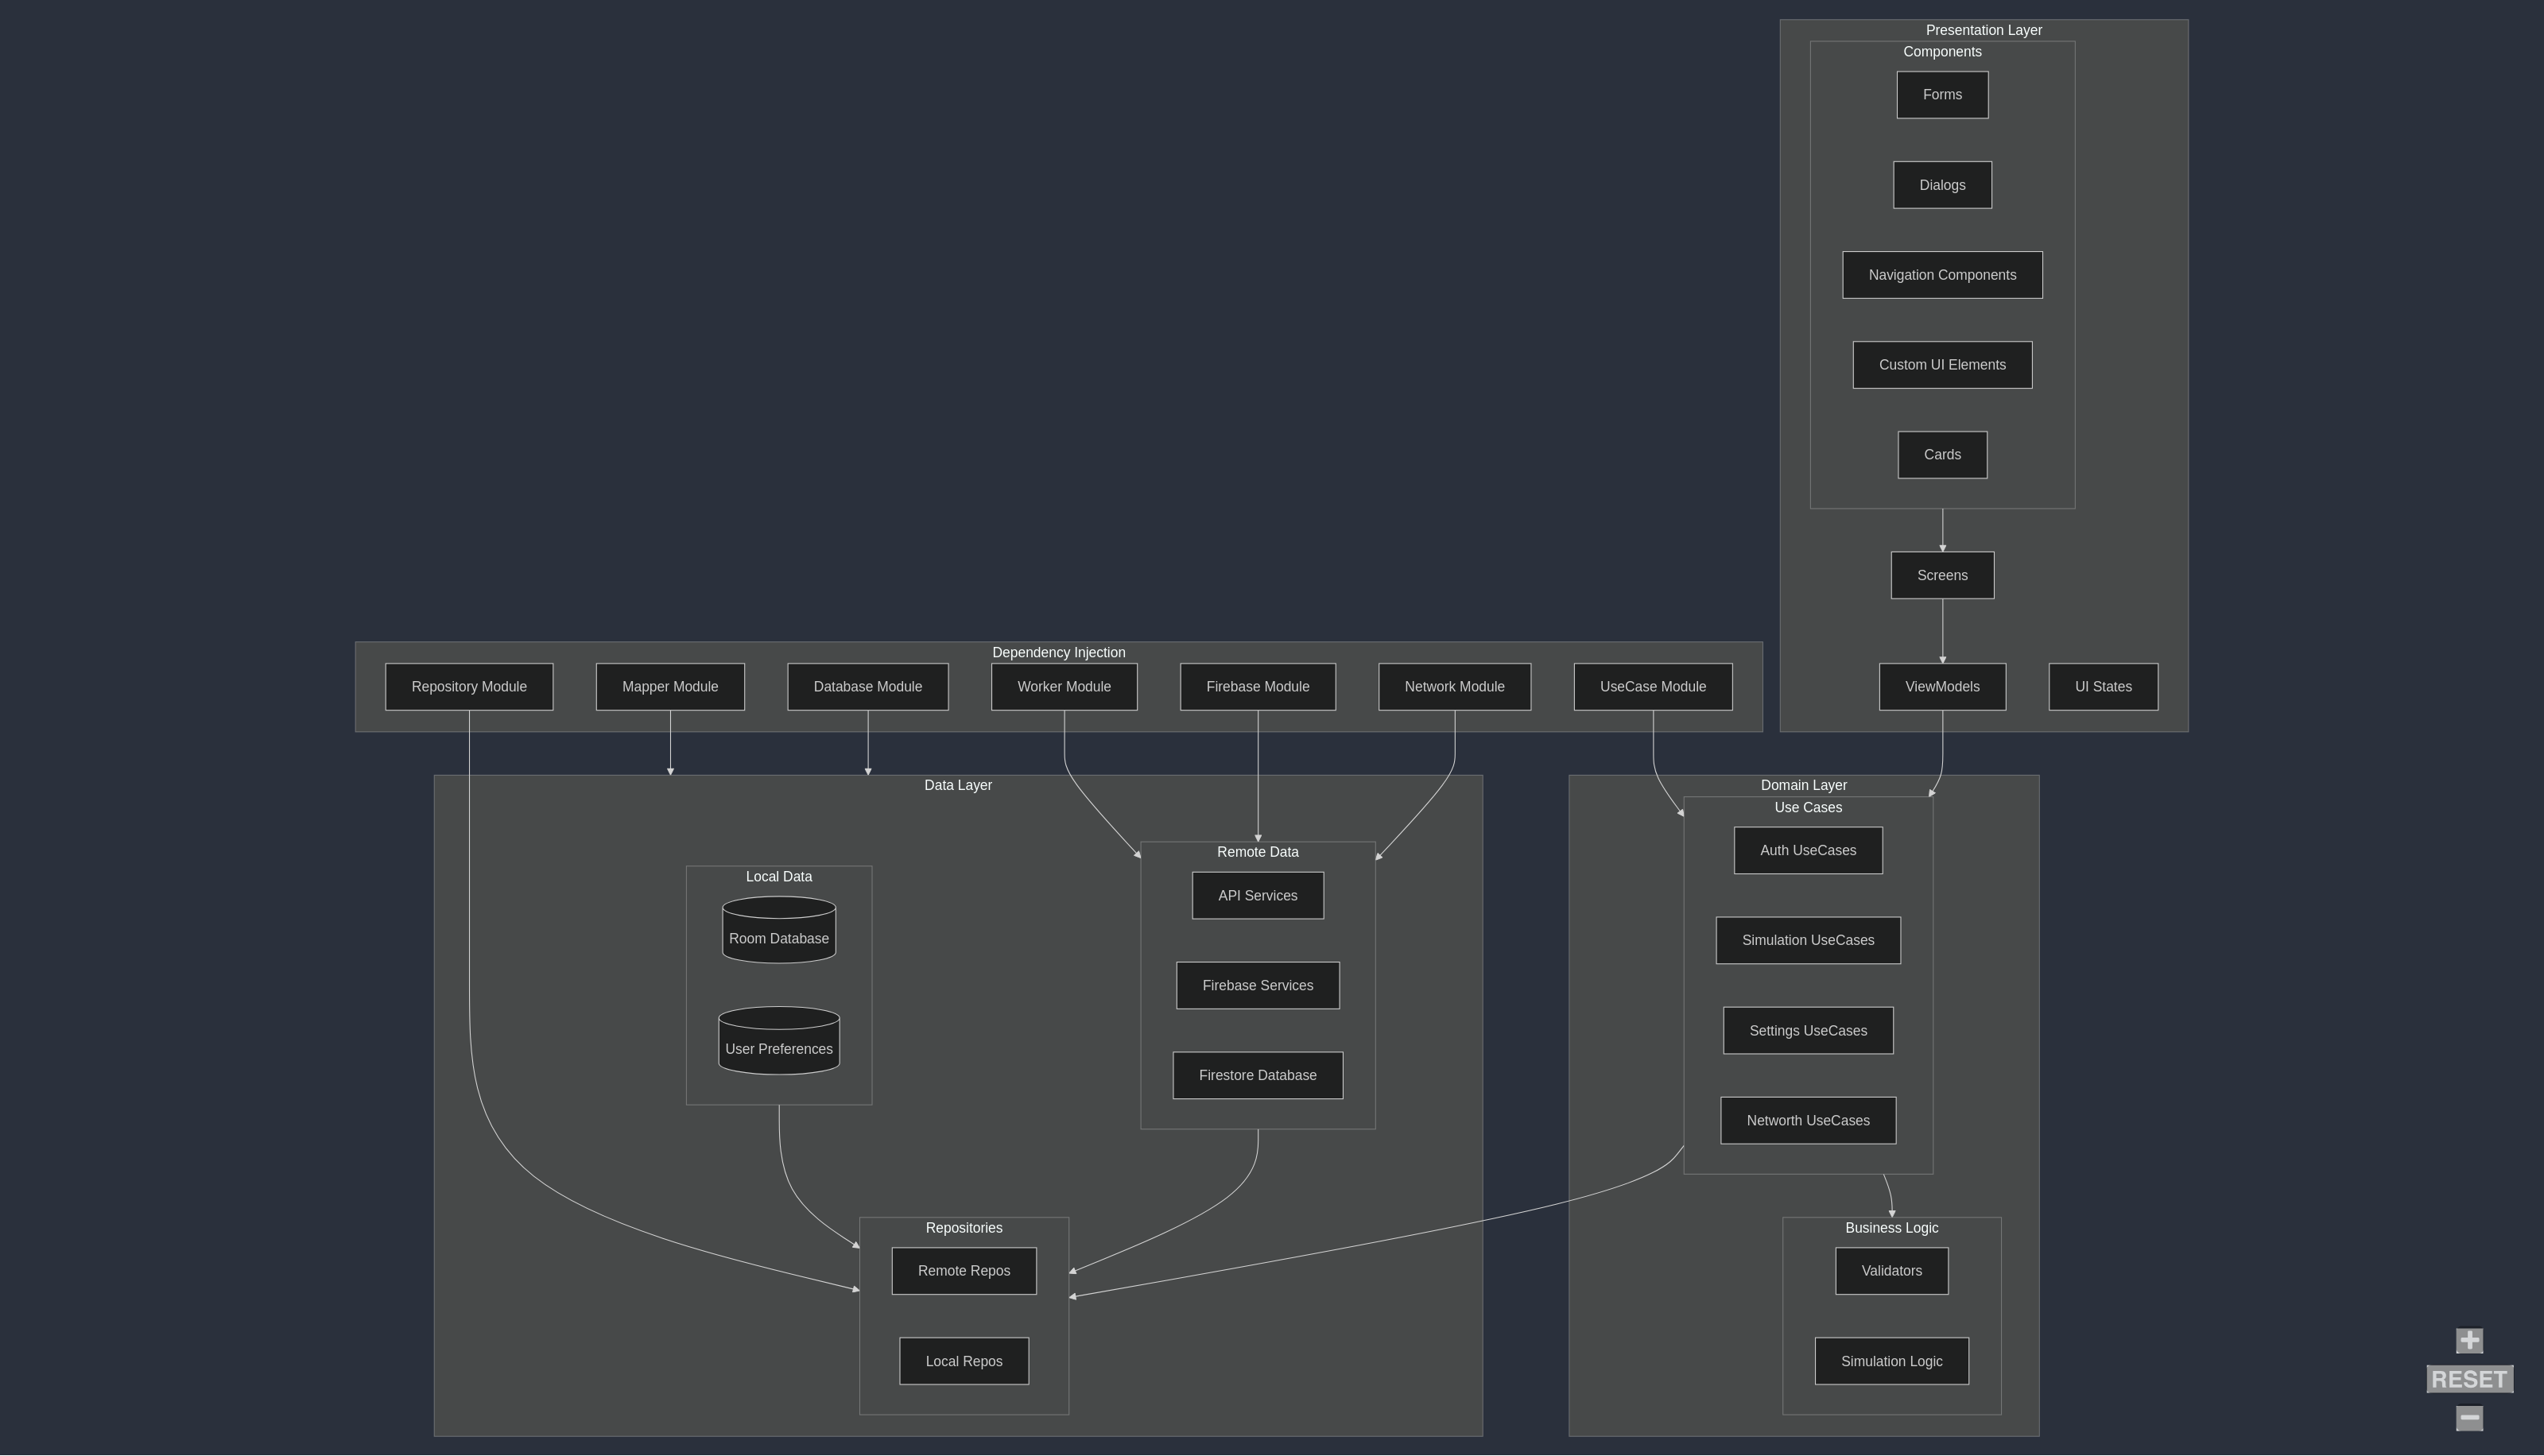
\includegraphics[width=1\textwidth]{foto/architecture}
    \caption{}
    \label{fig:architecture}
\end{figure}

\section*{Algoritmo di Simulazione FIRE (Financial Independence, Retire Early)}
\addcontentsline{toc}{section}{ALGORITMO DI SIMULAZIONE FIRE (FINANCIAL INDEPENDENCE, RETIRE EARLY)}
   
    \section{Preambolo}\label{sec:preambolo2}

Il movimento Financial Independence, Retire Early (FIRE) \\ enfatizza il
    raggiungimento dell'indipendenza finanziaria e il pensionamento
    significativamente prima delle tradizionali età pensionabili.
    Fondamentale
    per la pianificazione FIRE è valutare la sostenibilità di una strategia
    prescelta in varie condizioni economiche.
    La simulazione svolge un ruolo
    fondamentale, consentendo agli individui di modellare la crescita del
    portafoglio, stimare tassi di prelievo sicuri e tenere conto di incertezze
    come la volatilità del mercato e l'inflazione.
    Questo documento presenta una
    descrizione teorica dettagliata di un algoritmo di simulazione FIRE
    progettato per questo scopo.
    Mira a fornire una comprensione completa della
    meccanica, delle ipotesi e delle potenziali applicazioni della simulazione.

    \section{Panoramica dell'Algoritmo}\label{sec:panoramica-dell'algoritmo}

L'algoritmo di simulazione FIRE è una simulazione di Monte Carlo progettata per
modellare la performance di un portafoglio su un periodo di lungo termine,
tenendo conto dei rendimenti di mercato, dell'inflazione, dei prelievi e di
altri parametri finanziari rilevanti.
Il principio fondamentale è generare una
moltitudine di possibili scenari futuri (simulazioni) e valutare il
comportamento del portafoglio in ciascuno di essi.\ Analizzando i risultati di
queste simulazioni, è possibile stimare la probabilità di raggiungere
l'indipendenza finanziaria e di mantenere uno stile di vita desiderato per tutto
il periodo di pensionamento pianificato.

    La simulazione opera iterativamente, modellando l'evoluzione del portafoglio
    su base annuale (o potenzialmente a intervalli di tempo più granulari).
    Ogni
    esecuzione di simulazione rappresenta un possibile futuro unico, guidato da
    rendimenti di mercato e tassi di inflazione campionati casualmente.
    L'algoritmo tiene traccia del valore del portafoglio, delle riserve di
    liquidità e degli importi dei prelievi, valutando se il portafoglio rimane
    solvibile durante l'orizzonte di simulazione (in genere diversi decenni).

    L'output chiave della simulazione è un tasso di successo, che rappresenta la
    percentuale di simulazioni in cui il portafoglio rimane al di sopra dello
    zero (o una soglia minima predefinita) alla fine del periodo di simulazione.
    Questo tasso di successo funge da misura probabilistica della fattibilità
    del piano.

    \section{Componenti e Moduli
    Fondamentali}\label{sec:componenti-e-moduli-fondamentali}
    L'algoritmo di simulazione FIRE può essere concettualmente suddiviso in diversi
moduli chiave, ciascuno responsabile di un aspetto specifico del processo di
simulazione.
Questi moduli interagiscono tra loro per creare un modello completo
della performance del portafoglio.

    \subsection{Input e Configurazione dei
    Dati}\label{subsec:input-e-configurazione-dei-dati}

Questo modulo è responsabile della raccolta e della strutturazione dei dati di
input richiesti per la simulazione.
Questo include:
    \begin{itemize}
        \item \textbf{Valore Iniziale del Portafoglio:} Il valore iniziale del
        portafoglio di investimenti.
        \item \textbf{Riserve di Liquidità:} L'importo iniziale di liquidità
        detenuto al di fuori del portafoglio di investimenti.
        \item \textbf{Asset Allocation:} L'allocazione del portafoglio tra
        diverse classi di attività (ad esempio, azioni, obbligazioni, immobili).
        Questo influenza il rendimento atteso e la volatilità del portafoglio.
        \item \textbf{Strategia di Prelievo:} L'importo di prelievo annuale
        pianificato, potenzialmente adeguato per l'inflazione.
        Questo può essere
        un importo fisso, una percentuale del portafoglio o una strategia più
        complessa.
        \item \textbf{Modello di Inflazione:} Specifica di come vengono generati
        i tassi di inflazione (vedere la Sezione 3.3).
        \item \textbf{Parametri di Simulazione:} Parametri come la durata della
        simulazione (numero di anni), il numero di simulazioni da eseguire e il
        tasso di interesse sulla liquidità.
        \item \textbf{Tassi di Spesa:} Tassi di imposta, percentuali di imposta
        di bollo e percentuali di carico applicate ai valori degli investimenti
        o alle transazioni.
        \item \textbf{Impostazioni Intervallo di Pensionamento:} Specifica gli
        anni fino al pensionamento completo e il numero di anni nel
        pensionamento completo.
        \item \textbf{Dati Storici di Mercato:} Dati di serie temporali che
        rappresentano i rendimenti storici del mercato per le classi di attività
        scelte.
        \item \textbf{Dati Storici sull'Inflazione:} Dati di serie temporali che
        rappresentano i tassi di inflazione storici.
    \end{itemize}

    Il modulo di input dei dati garantisce che tutte le informazioni necessarie
    siano disponibili in un formato coerente e facilmente accessibile per le
    fasi di simulazione successive.

    \subsection{Modello di Rendimento di
    Mercato}\label{subsec:modello-di-rendimento-di-mercato}

Questo modulo è responsabile della generazione di una serie di rendimenti di
mercato per ciascuna classe di attività nel portafoglio per ogni anno della
simulazione.
Una modellazione accurata dei rendimenti di mercato è fondamentale
per simulare la crescita del portafoglio in varie condizioni di mercato.

    Un approccio comune è utilizzare i dati storici di mercato per generare una
    distribuzione di potenziali rendimenti.
    Questo può essere fatto usando varie
    tecniche:
    \begin{itemize}
        \item \textbf{Campionamento Storico (Bootstrapping):} Campionamento
        casuale dei rendimenti direttamente dai dati storici.
        Questo approccio
        presuppone che il comportamento futuro del mercato assomigli al
        comportamento passato.
        Una variante è il Block Bootstrap dove vengono
        campionati blocchi di periodi di tempo invece di singoli periodi di
        tempo.
        \item \textbf{Modellazione Parametrica:} Adattare una distribuzione
        statistica (ad esempio, distribuzione normale, distribuzione lognormale)
        ai dati storici e generare rendimenti casuali da tale distribuzione.
        Ciò
        richiede la stima dei parametri della distribuzione (ad esempio, media,
        deviazione standard).
        \item \textbf{Modelli di Serie Temporali:} Utilizzare modelli di serie
        temporali più sofisticati (ad esempio, ARMA, GARCH) per prevedere i
        rendimenti futuri sulla base dei dati passati e delle relazioni
        statistiche.
    \end{itemize}

    L'output chiave del modello di rendimento di mercato è una matrice di
    rendimenti, in cui ogni riga rappresenta un anno nella simulazione e ogni
    colonna rappresenta una diversa esecuzione della simulazione.

    Matematicamente, se \(R_{t,s}\) è il rendimento dell'asset durante l'anno
    \(t\) nella simulazione \(s\), allora il valore di un portafoglio investito
    in quell'asset crescerà di
    \[
    V_{t+1,s} = V_{t,s} \cdot (1 + R_{t,s}),
    \]
    dove \(V_{t,s}\) è il valore del portafoglio all'anno \(t\) nella
    simulazione \(s\).
    Per un portafoglio multi-asset, viene calcolata una media
    ponderata dei rendimenti di mercato specifici dell'asset.

    \subsection{Modello di Inflazione}\label{subsec:modello-di-inflazione}

L'inflazione erode il potere d'acquisto del denaro nel tempo, quindi è
essenziale incorporare l'inflazione nella simulazione.\ Il modello di inflazione
genera una serie di tassi di inflazione per ogni anno della simulazione.

Simile ai rendimenti di mercato, è possibile utilizzare vari approcci:
\begin{itemize}
    \item \textbf{Campionamento Storico:} Campionare casualmente i tassi di
    inflazione direttamente dai dati storici sull'inflazione.
    \item \textbf{Modellazione Parametrica:} Adattare una distribuzione
    statistica ai dati storici sull'inflazione e generare tassi di inflazione
    casuali da tale distribuzione.
    Una distribuzione log-normale viene spesso
    utilizzata perché i tassi di inflazione non possono essere negativi.
    \item \textbf{Tasso di Inflazione Fisso:} Assumere un tasso di inflazione
    medio costante per tutti gli anni.
    Questo fornisce uno scenario di base
    semplice.
    \item \textbf{Dati Storici Scalati:} Scala i tassi di inflazione campionati
    per soddisfare un tasso di inflazione medio specificato.
    \item \textbf{Modello Lognormale:} Il modello lognormale assume che i tassi
    di inflazione seguano una distribuzione lognormale, che è particolarmente
    adatta poiché:
    \begin{itemize}
        \item Genera solo valori positivi, coerentemente con la natura
        dell'inflazione
        \item È asimmetrica verso destra, catturando eventi di alta inflazione
        occasionale
        \item Ha una base teorica nel teorema del limite centrale per processi
        moltiplicativi
    \end{itemize}
\end{itemize}

Matematicamente, sia \(I_{t,s}\) a rappresentare il tasso di inflazione per
l'anno \(t\) nella simulazione \(s\).
Un tasso di prelievo nell'anno \(t\) di
\(W_{t,s}\) avrà il potere d'acquisto di
\[
\frac{W_{t,s}}{1+I_{t,s}}
\]
nel valore della valuta dell'anno \(t+1\).

Nel caso del modello lognormale, se \(X\) segue una distribuzione lognormale con
parametri \(\mu\) e \(\sigma\), allora:
\begin{gather*}
    E[X] = e^{\mu + \frac{\sigma^2}{2}}\\
    Var(X) = (e^{\sigma^2} - 1)e^{2\mu + \sigma^2}\\
\end{gather*}

I parametri \(\mu\) e \(\sigma\) vengono calibrati per ottenere il tasso medio
di inflazione desiderato e la varianza storica osservata.

    \subsection{Modello di Prelievo}\label{subsec:modello-di-prelievo}

Il modello di prelievo definisce la quantità di denaro prelevata dal portafoglio
ogni anno per coprire le spese di soggiorno.
La strategia di prelievo può
influenzare significativamente il tasso di successo del piano FIRE. Le strategie
di prelievo comuni includono:
    \begin{itemize}
        \item \textbf{Importo Fisso:} Un importo fisso in dollari viene
        prelevato ogni anno, potenzialmente adeguato per l'inflazione.
        \item \textbf{Strategie di Prelievo Dinamiche:} Strategie più
        sofisticate che adeguano i prelievi in base alle condizioni di mercato,
        al valore del portafoglio e ad altri fattori.
        Ad esempio, ridurre i
        prelievi durante le fasi di ribasso del mercato.
    \end{itemize}

    La rappresentazione matematica del modello di prelievo dipende dalla
    strategia scelta.
    Per un importo fisso adeguato per l'inflazione, l'importo
    del prelievo \(W_{t,s}\) per l'anno \(t\) nella simulazione \(s\) può essere
    espresso come:
    \[
    W_{t,s} = W_0 \cdot \prod_{i=1}^{t} (1 + I_{i,s}),
    \]
    dove \(W_0\) è l'importo del prelievo iniziale e \(I_{i,s}\) è il tasso di
    inflazione per l'anno \(i\) nella simulazione \(s\).
    Per un prelievo basato
    sulla percentuale, l'importo del prelievo è:
    \[
    W_{t,s} = p \cdot V_{t,s},
    \]
    dove \(p\) è la percentuale di prelievo e \(V_{t,s}\) è il valore del
    portafoglio all'inizio dell'anno \(t\) nella simulazione \(s\).

    \subsection{Modello di Evoluzione del
    Portafoglio}\label{subsec:modello-di-evoluzione-del-portafoglio}

Questo è il motore di simulazione principale che tiene traccia della performance
del portafoglio nel tempo.
Per ogni anno in ogni simulazione, l'algoritmo esegue
i seguenti passaggi:
    \begin{enumerate}
        \item \textbf{Calcola i Rendimenti degli Investimenti:} Applica i
        rendimenti di mercato per l'anno alle attività del portafoglio,
        adeguando per l'asset allocation.
        \item \textbf{Adatta per l'Inflazione:} Prendi in considerazione
        l'impatto dell'inflazione dell'anno in corso.
        \item \textbf{Preleva Fondi:} Preleva l'importo pianificato in base alla
        strategia di prelievo.
        \item \textbf{Calcola Imposte e Spese:} Calcola e detrai eventuali
        imposte applicabili (ad esempio, l'imposta sulle plusvalenze) e le spese
        (ad esempio, le commissioni di gestione).
        \item \textbf{Aggiorna il Valore del Portafoglio:} Aggiorna il valore
        del portafoglio per riflettere i rendimenti degli investimenti, i
        prelievi, le imposte e le spese.
        \item \textbf{Aggiorna le Riserve di Liquidità:} Aggiorna le riserve di
        liquidità se vengono trasferiti fondi da/verso il portafoglio di
        investimenti.
    \end{enumerate}

    L'equazione fondamentale che governa l'evoluzione del portafoglio può essere
    espressa come:
    \[
    V_{t+1,s} = V_{t,s} \cdot (1 + R_{t,s}) - W_{t,s} - T_{t,s},
    \]
    dove:
    \begin{itemize}
        \item \(V_{t+1,s}\) è il valore del portafoglio alla fine dell'anno
        \(t\) nella simulazione \(s\).
        \item \(V_{t,s}\) è il valore del portafoglio all'inizio dell'anno \(t\)
        nella simulazione \(s\).
        \item \(R_{t,s}\) è il rendimento di mercato per l'anno \(t\) nella
        simulazione \(s\).
        \item \(W_{t,s}\) è l'importo del prelievo per l'anno \(t\) nella
        simulazione \(s\).
        \item \(T_{t,s}\) sono le imposte e le spese totali per l'anno \(t\)
        nella simulazione \(s\).
    \end{itemize}

    L'algoritmo ripete questi passaggi per ogni anno nell'orizzonte di
    simulazione e per ogni esecuzione di simulazione.

    \subsection{Calcolo del Tasso di
    Successo}\label{subsec:calcolo-del-tasso-di-successo}

Dopo aver completato tutte le esecuzioni della simulazione, il tasso di successo
viene calcolato determinando la percentuale di simulazioni in cui il portafoglio
rimane solvibile alla fine del periodo di simulazione.

    Una simulazione è tipicamente considerata riuscita se il valore del
    portafoglio rimane al di sopra dello zero (o di una soglia minima
    predefinita) alla fine dell'orizzonte di simulazione.
    Il tasso di successo
    viene quindi calcolato come:
    \[
    \text{Tasso di Successo} = \frac{\text{Numero di Simulazioni Riuscite}}{\text{Numero Totale di Simulazioni}} \times 100\%
    \]
    Il tasso di successo fornisce una misura probabilistica della fattibilità
    del piano FIRE. Un tasso di successo più elevato indica una maggiore
    probabilità di raggiungere l'indipendenza finanziaria e di mantenere lo
    stile di vita desiderato per tutto il periodo di pensionamento.

    \section{Assunzioni e Limitazioni}\label{sec:assunzioni-e-limitazioni}

L'algoritmo di simulazione FIRE si basa su diverse assunzioni che possono
influire sull'accuratezza dei risultati:
    \begin{itemize}
        \item \textbf{Dati Storici di Mercato:} L'algoritmo si basa spesso sui
        dati storici di mercato per modellare i rendimenti futuri.
        Le
        performance passate non sono necessariamente indicative dei risultati
        futuri e cambiamenti significativi nelle condizioni di mercato possono
        invalidare queste assunzioni.
        \item \textbf{Modellazione dell'Inflazione:} Allo stesso modo, il
        modello di inflazione si basa sui dati storici sull'inflazione.
        Cambiamenti imprevisti dell'inflazione possono influire
        significativamente sui risultati.
        \item \textbf{Strategia di Prelievo:} Si presuppone che la strategia di
        prelievo scelta sia costante per tutta la simulazione.
        Cambiamenti nelle
        abitudini di spesa o spese impreviste possono influire sulla
        sostenibilità del piano FIRE\@.
        \item \textbf{Leggi Fiscali e Regolamenti:} L'algoritmo presuppone che
        le leggi fiscali e i regolamenti rimarranno costanti per tutta la
        simulazione.
        Cambiamenti nelle politiche fiscali possono influire sulla
        crescita e sugli importi dei prelievi del portafoglio.
        \item \textbf{Commissioni di Investimento:} Il modello potrebbe
        semplificare il trattamento delle commissioni di investimento.
        È
        importante garantire che il modello li prenda in considerazione in modo
        accurato.
        \item \textbf{Eventi Cigno Nero:} Il modello non può prevedere o tenere
        conto di eventi \("\)cigno nero\("\) imprevisti (ad esempio, grandi
        crisi economiche, eventi geopolitici) che possono avere un impatto
        significativo sui rendimenti di mercato e sull'inflazione.
    \end{itemize}

    È fondamentale comprendere queste limitazioni e interpretare i risultati
    della simulazione con cautela.
    L'algoritmo di simulazione FIRE fornisce uno
    strumento prezioso per valutare la fattibilità dei piani FIRE, ma non deve
    essere considerato un predittore definitivo dei risultati futuri.

    \section{Considerazioni Avanzate}\label{sec:considerazioni-avanzate}

Oltre ai componenti principali descritti sopra, diverse considerazioni avanzate
possono essere incorporate nell'algoritmo di simulazione FIRE per migliorarne il
realismo e l'accuratezza:
    \begin{itemize}
        \item \textbf{Asset Allocation Dinamica:} Adeguare l'asset allocation
        nel tempo in base alle condizioni di mercato o alla fase di
        pensionamento.
        Ad esempio, passare dalle azioni alle obbligazioni quando
        ci si avvicina alla pensione.
        \item \textbf{Rischio della Sequenza dei Rendimenti:} Tenere conto
        dell'impatto della sequenza dei rendimenti, in cui i rendimenti negativi
        all'inizio del pensionamento possono avere un impatto
        sproporzionatamente grande sulla sostenibilità del portafoglio.
        \item \textbf{Riduzione della Varianza di Monte Carlo:} Tecniche per
        migliorare l'efficienza delle simulazioni di Monte Carlo riducendo la
        varianza delle stime.
        \item \textbf{Modellazione Dettagliata delle Imposte:} Modellazione più
        dettagliata delle imposte e dei regolamenti specifici che influiscono
        sui rendimenti degli investimenti e sui prelievi, potenzialmente
        personalizzata per giurisdizioni specifiche.
        \item \textbf{Incorporare Altre Fonti di Reddito:} Tenere conto di altre
        fonti di reddito, come pensioni, previdenza sociale o lavoro part-time,
        nel modello di prelievo.
        \item \textbf{Shock di Spesa:} Simulare spese impreviste (ad esempio,
        emergenze mediche, riparazioni domestiche) e il loro impatto sul piano
        FIRE\@.
    \end{itemize}

    \section{Considerazioni}\label{sec:considerazioni2}

L'algoritmo di simulazione FIRE è un potente strumento per valutare la
fattibilità dei piani FIRE. Modellando la performance del portafoglio in varie
condizioni di mercato, tassi di inflazione e strategie di prelievo, fornisce una
misura probabilistica della probabilità di raggiungere l'indipendenza
finanziaria e di mantenere uno stile di vita desiderato per tutto il periodo di
pensionamento.
Questo documento ha fornito una descrizione teorica completa dei
componenti, delle assunzioni e delle limitazioni dell'algoritmo, consentendo una
comprensione più approfondita della sua meccanica e delle sue applicazioni.
È
importante notare che l'algoritmo descritto è più utile quando è adattato alle
circostanze personali e utilizzato per mettere alla prova le assunzioni per
scenari futuri. \section*{Sistema di Sincronizzazione Dati Locale-Remoto}
\addcontentsline{toc}{section}{SISTEMA DI SINCRONIZZAZIONE DATI LOCALE-REMOTO)}

\section{Preambolo}\label{sec:preambolo3} La sincronizzazione dati tra app
mobile e DB remoto è cruciale.
Usiamo Android WorkManager e \texttt{SyncWorker}
per ADD, UPDATE, DELETE. La coda di sincronizzazione è gestita con
\texttt{SyncQueueItem}.

\section{Architettura del Sistema}\label{sec:architettura-del-sistema} Tre
componenti:
\begin{itemize}
    \item \textbf{SyncWorker}: Esegue la sincronizzazione.
    Usa
    \texttt{FirestoreRepository} e \texttt{LocalDatabaseRepository}.
    \item \textbf{SyncQueueItem}: Operazione in sospeso.
    Contiene ID,
    collezione, payload, tipo operazione, stato.
    \item \textbf{SyncQueueItemRepository}: Gestisce la coda di sincronizzazione
    nel DB locale.
\end{itemize}

\section{Componenti del Sistema}\label{sec:componenti-del-sistema}
\subsection{SyncWorker}\label{subsec:syncworker} Gestisce la sincronizzazione.
Usa Hilt.

\begin{lstlisting}[caption=SyncWorker.kt, label=lst:syncworker, basicstyle=\ttfamily\scriptsize, breaklines=true, breakatwhitespace=true, tabsize=4]
@HiltWorker class SyncWorker<T> @AssistedInject constructor( @Assisted context:
Context, @Assisted workerParams: WorkerParameters, private val
syncQueueItemRepository: SyncQueueItemRepository, private val
firestoreRepository: FirestoreRepository, private val localRepository:
LocalDatabaseRepository<T> ) : CoroutineWorker(context, workerParams) {
companion object { private const val TAG = "SyncWorker" }

    override suspend fun doWork(): Result = coroutineScope { try { Log.d(TAG,
        "Starting sync work") cleanupStuckSyncingItems()

            val currentTime = System.currentTimeMillis() val pendingItems =
            syncQueueItemRepository.getPendingItems(currentTime) Log.d(TAG,
            "Found ${pendingItems.size} pending items ready for processing")

            if (pendingItems.isEmpty()) { Log.d(TAG, "No pending items,
                completing successfully") return@coroutineScope Result.success()
                }

            val results = processBatches(pendingItems) Log.d(TAG, "Processed
            ${results.size} items")

            val errorCount = results.count { it is SyncOperationResult.Error }
            val successCount = results.count { it is SyncOperationResult.Success
            } val retryCount = results.count { it is SyncOperationResult.Retry }
            val staleCount = results.count { it is SyncOperationResult.StaleData
            }

            Log.d(TAG, "Sync results - Success: $successCount, Errors:
            $errorCount, Retries: $retryCount, Stale: $staleCount")

            handleFailedItems()

            return@coroutineScope when { errorCount > 0 -> { Log.w(TAG, "Some
                operations failed, scheduling retry") Result.retry() }
                staleCount > 0 -> { Log.d(TAG, "Some items were stale and have
                been handled") Result.success() } else -> { Log.d(TAG, "All
                operations completed successfully") Result.success() } } } catch
                (e: Exception) { handleWorkerError(e) } } // ... (rest of the
                code) }
\end{lstlisting}

\textbf{doWork()}: Sovrascrive \texttt{doWork()}.
Passaggi:
\begin{enumerate}
    \item \textbf{cleanupStuckSyncingItems()}: Pulisce elementi bloccati in
    \texttt{SYNCING}.
    \item \textbf{Recupera elementi in sospeso}: Ottiene elementi pronti.
    \item \textbf{Elabora i batch}: Divide in batch.
    \item \textbf{Gestisce i risultati}: Gestisce successo, errore, retry.
    \item \textbf{handleFailedItems()}: Elimina tentativi massimi superati.
    \item \textbf{Restituisce il risultato}: \texttt{Result.success()},
    \texttt{Result.retry()} o \texttt{Result.failure()}.
\end{enumerate}

\textbf{Operazioni di sincronizzazione}:

\begin{lstlisting}[caption=Operazioni di Sincronizzazione, label=lst:sync_operations, basicstyle=\ttfamily\scriptsize, breaklines=true, breakatwhitespace=true, tabsize=4]
    private suspend fun performAddOperation(item: SyncQueueItem):
        SyncOperationResult { Log.d(TAG, "Performing ADD operation for item
        ${item.id}") return firestoreRepository.addDocument(collectionPath =
        item.collection, data = item.payload, documentId =
        item.id).first().fold( onSuccess = { Log.d(TAG, "ADD operation
        successful for item ${item.id}"); SyncOperationResult.Success(item.id)
        }, onFailure = { error -> Log.e(TAG, "ADD operation failed for item
        ${item.id}", error); throw error } ) }

    private suspend fun performUpdateOperation(item: SyncQueueItem):
        SyncOperationResult { Log.d(TAG, "Performing UPDATE operation for item
        ${item.id}") try { val currentDocResult =
        firestoreRepository.getDocumentById(collectionPath = item.collection,
        documentId = item.id).first() val currentDoc =
        currentDocResult.getOrNull() ?: throw IllegalStateException("Remote
        document not found or null") val remoteTimestamp =
        (currentDoc["updatedAt"] as? Double)?.toLong() ?: throw
        IllegalStateException("Remote document missing updatedAt timestamp") val
        localTimestamp = item.createdAt if (remoteTimestamp > localTimestamp) {
        Log.d("UpdateUserSettingsUseCase", "Remote document is newer (remote:
        $remoteTimestamp, local: $localTimestamp)") return
        SyncOperationResult.StaleData(item.id) } return
        firestoreRepository.updateDocument(collectionPath = item.collection,
        data = item.payload, documentId = item.id).first().fold( onSuccess = {
        Log.d(TAG, "UPDATE operation successful for item ${item.id}");
        SyncOperationResult.Success(item.id) }, onFailure = { error ->
        Log.e(TAG, "UPDATE operation failed for item ${item.id}", error); throw
        error } ) } catch (e: Exception) { Log.e(TAG, "Error during UPDATE
        operation for item ${item.id}", e); throw e } }

    private suspend fun performDeleteOperation(item: SyncQueueItem):
        SyncOperationResult { Log.d(TAG, "Performing DELETE operation for item
        ${item.id}") return firestoreRepository.deleteDocument(collectionPath =
        item.collection, documentId = item.id).first().fold( onSuccess = {
        Log.d(TAG, "DELETE operation successful for item ${item.id}");
        SyncOperationResult.Success(item.id) }, onFailure = { error ->
        Log.e(TAG, "DELETE operation failed for item ${item.id}", error); throw
        error } ) }
\end{lstlisting}

\subsection{SyncQueueItem}\label{subsec:syncqueueitem} Rappresenta un'operazione
di sincronizzazione.

\begin{lstlisting}[caption=SyncQueueItem.kt, label=lst:syncqueueitem, basicstyle=\ttfamily\scriptsize, breaklines=true, breakatwhitespace=true, tabsize=4]
package com.unimib.ignitionfinance.data.local.entity

import androidx.room.ColumnInfo import androidx.room.Entity import
androidx.room.PrimaryKey import
com.unimib.ignitionfinance.data.local.utils.SyncStatus

@Entity(tableName = "sync_queue_items") data class SyncQueueItem ( @PrimaryKey
val id: String, @ColumnInfo(name = "collection") val collection: String,
@ColumnInfo(name = "payload") val payload: Map<String, Any>, @ColumnInfo(name =
"operation") val operationType: String, @ColumnInfo(name = "status") val status:
SyncStatus = SyncStatus.PENDING, @ColumnInfo(name = "attempts") val attempts:
Int = 0, @ColumnInfo(name = "created_at") val createdAt: Long =
System.currentTimeMillis(), @ColumnInfo(name = "scheduled_for") val
scheduledFor: Long = System.currentTimeMillis() )
\end{lstlisting}

\textbf{Campi principali}:
\begin{itemize}
    \item \texttt{id}: ID univoco.
    \item \texttt{collection}: Nome collezione Firestore.
    \item \texttt{payload}: Dati da sincronizzare.
    \item \texttt{operationType}: ADD, UPDATE, DELETE\@.
    \item \texttt{status}: PENDING, SYNCING, SUCCEEDED, FAILED\@.
    \item \texttt{attempts}: Numero di tentativi.
    \item \texttt{createdAt}: Timestamp creazione.
    \item \texttt{scheduledFor}: Timestamp schedulato.
\end{itemize}

\subsection{SyncQueueItemRepository}\label{subsec:syncqueueitemrepository}
Fornisce accesso al DB locale.

\begin{lstlisting}[caption=SyncQueueItemDao.kt, label=lst:syncqueueitemdao, basicstyle=\ttfamily\scriptsize, breaklines=true, breakatwhitespace=true, tabsize=4]
package com.unimib.ignitionfinance.data.local.database

import androidx.room.Dao import androidx.room.Delete import androidx.room.Insert
import androidx.room.OnConflictStrategy import androidx.room.Query import
androidx.room.Update import
com.unimib.ignitionfinance.data.local.entity.SyncQueueItem import
com.unimib.ignitionfinance.data.local.utils.SyncStatus

@Dao interface SyncQueueItemDao { @Insert(onConflict =
OnConflictStrategy.REPLACE) suspend fun insert(item: SyncQueueItem)

    @Update suspend fun update(item: SyncQueueItem)

    @Delete suspend fun delete(item: SyncQueueItem)

    @Query("SELECT * FROM sync_queue_items WHERE id = :id") suspend fun
    getById(id: String): SyncQueueItem?

    @Query("SELECT * FROM sync_queue_items WHERE status = :status") suspend fun
    getByStatus(status: SyncStatus): List<SyncQueueItem>

    @Query("SELECT * FROM sync_queue_items WHERE status = :status AND collection
    = :collection") suspend fun getByStatusAndCollection(status: SyncStatus,
    collection: String): List<SyncQueueItem>

    @Query("SELECT * FROM sync_queue_items WHERE scheduled_for <= :timestamp AND
    status = :status") suspend fun getPendingItems(timestamp: Long =
    System.currentTimeMillis(), status: SyncStatus = SyncStatus.PENDING):
    List<SyncQueueItem>

    @Query("SELECT * FROM sync_queue_items WHERE attempts >= :maxAttempts AND
    status = :status") suspend fun getFailedItems(maxAttempts: Int, status:
    SyncStatus = SyncStatus.FAILED): List<SyncQueueItem> }
\end{lstlisting}

\textbf{Metodi principali}:
\begin{itemize}
    \item \texttt{insert(item)}: Inserisce.
    \item \texttt{update(item)}: Aggiorna.
    \item \texttt{delete(item)}: Elimina.
    \item \texttt{getById(id)}: Recupera per ID\@.
    \item \texttt{getByStatus(status)}: Recupera per stato.
    \item \texttt{getPendingItems(timestamp)}: Recupera in sospeso.
\end{itemize}

\subsection{SyncOperationScheduler}\label{subsec:syncoperationscheduler}
Gestisce pianificazione con WorkManager.

\begin{lstlisting}[caption=SyncOperationScheduler.kt, label=lst:syncoperationscheduler, basicstyle=\ttfamily\scriptsize, breaklines=true, breakatwhitespace=true, tabsize=4]
package com.unimib.ignitionfinance.data.remote.worker

import android.content.Context import androidx.work.BackoffPolicy import
androidx.work.Constraints import androidx.work.ExistingPeriodicWorkPolicy import
androidx.work.NetworkType import androidx.work.OneTimeWorkRequestBuilder import
androidx.work.PeriodicWorkRequestBuilder import androidx.work.WorkManager import
java.util.concurrent.TimeUnit

object SyncOperationScheduler { const val TAG = "SyncOperationScheduler" const
    val SYNC_WORK_NAME = "sync_operation_work" const val MAX_RETRIES = 3 const
    val SYNC_TIMEOUT_MS = 30000L const val BATCH_SIZE = 10 const val
    BATCH_DELAY_MS = 1000L const val INITIAL_BACKOFF_DELAY_MS = 10000L const val
    PERIODIC_SYNC_INTERVAL = 15L const val MIN_BACKOFF_DELAY_MS = 5000L const
    val MAX_BACKOFF_DELAY_MS = 300000L

    inline fun <reified T> schedule(context: Context, constraints: Constraints =
        getDefaultConstraints()) { Log.d(TAG, "Scheduling periodic sync work
        with interval: $PERIODIC_SYNC_INTERVAL minutes") try { val
        syncWorkRequest =
        PeriodicWorkRequestBuilder<SyncWorker<T>>(repeatInterval =
        PERIODIC_SYNC_INTERVAL, repeatIntervalTimeUnit = TimeUnit.MINUTES,
        flexTimeInterval = 5, flexTimeIntervalUnit = TimeUnit.MINUTES)
        .setConstraints(constraints)
        .setBackoffCriteria(BackoffPolicy.EXPONENTIAL, INITIAL_BACKOFF_DELAY_MS,
        TimeUnit.MILLISECONDS) .build() Log.d(TAG, "Work request built with
        constraints: ${constraints.requiredNetworkType}")
        WorkManager.getInstance(context).enqueueUniquePeriodicWork(SYNC_WORK_NAME,
        ExistingPeriodicWorkPolicy.REPLACE, syncWorkRequest) Log.i(TAG,
        "Periodic sync work scheduled successfully") } catch (e: Exception) {
        Log.e(TAG, "Error scheduling periodic sync work", e) } }

    inline fun <reified T> scheduleOneTime(context: Context, constraints:
        Constraints = getDefaultConstraints()) { Log.d(TAG, "Scheduling one-time
        sync work with initial delay: $initialDelay ms") try { val
        syncWorkRequest = OneTimeWorkRequestBuilder<SyncWorker<T>>()
        .setConstraints(constraints)
        .setBackoffCriteria(BackoffPolicy.EXPONENTIAL,
        INITIAL_BACKOFF_DELAY_MS.coerceIn(MIN_BACKOFF_DELAY_MS,
        MAX_BACKOFF_DELAY_MS), TimeUnit.MILLISECONDS)
        .setInitialDelay(initialDelay, TimeUnit.MILLISECONDS) .build()
        Log.d(TAG, "One-time work request built with constraints:
        ${constraints.requiredNetworkType}")
        WorkManager.getInstance(context).enqueue(syncWorkRequest) Log.i(TAG,
        "One-time sync work scheduled successfully") } catch (e: Exception) {
        Log.e(TAG, "Error scheduling one-time sync work", e) } }

    fun cancel(context: Context) { Log.d(TAG, "Cancelling sync work:
        $SYNC_WORK_NAME") try {
        WorkManager.getInstance(context).cancelUniqueWork(SYNC_WORK_NAME)
        Log.i(TAG, "Sync work cancelled successfully") } catch (e: Exception) {
        Log.e(TAG, "Error cancelling sync work", e) } }

    fun getDefaultConstraints() =
Constraints.Builder().setRequiredNetworkType(NetworkType.CONNECTED).setRequiresBatteryNotLow(true).build()
}
\end{lstlisting}

\textbf{Metodi principali}:
\begin{itemize}
    \item \texttt{schedule(context, constraints)}: Pianifica periodica.
    \item \texttt{scheduleOneTime(context, constraints)}: Pianifica una tantum.
    \item \texttt{cancel(context)}: Annulla.
    \item \texttt{getDefaultConstraints()}: Restituisce constraints predefinite.
\end{itemize}

\subsection{SyncOperationResult}\label{subsec:syncoperationresult} Risultato di
un'operazione.

\begin{lstlisting}[caption=SyncOperationResult.kt, label=lst:syncoperationresult, basicstyle=\ttfamily\scriptsize, breaklines=true, breakatwhitespace=true, tabsize=4]
package com.unimib.ignitionfinance.data.remote.worker

sealed class SyncOperationResult { data class Success(val itemId: String) :
    SyncOperationResult() data class Retry(val itemId: String, val error:
    Throwable) : SyncOperationResult() data class Error(val itemId: String, val
    error: Throwable) : SyncOperationResult() data class StaleData(val itemId:
    String) : SyncOperationResult() }
\end{lstlisting}

\textbf{Possibili risultati}:
\begin{itemize}
    \item \texttt{Success(itemId)}: Successo.
    \item \texttt{Retry(itemId, error)}: Riprova.
    \item \texttt{Error(itemId, error)}: Errore.
    \item \texttt{StaleData(itemId)}: Dati obsoleti.
\end{itemize}

\section{Flusso di Sincronizzazione}\label{sec:flusso-di-sincronizzazione}
\begin{enumerate}
    \item \textbf{Aggiunta/Modifica/Eliminazione}: Interazione utente.
    \item \textbf{Creazione SyncQueueItem}: Creazione elemento nella coda.
    \item \textbf{Pianificazione del Worker}: \texttt{SyncOperationScheduler}
    pianifica \texttt{SyncWorker}.
    \item \textbf{Esecuzione del Worker}:
    \begin{enumerate}
        \item \texttt{SyncWorker} recupera \texttt{SyncQueueItem} in stato
        \texttt{PENDING}.
        \item Esegue ADD, UPDATE, DELETE su Firestore.
        \item In caso di successo, aggiorna lo stato a \texttt{SUCCEEDED}.
        \item In caso di errore, aggiorna lo stato a \texttt{FAILED} e pianifica
        un retry.
    \end{enumerate}
    \item \textbf{Retry e Gestione Errori}: WorkManager gestisce i retry.
\end{enumerate}

\section{Gestione Errori e Retry}\label{sec:gestione-errori-e-retry}
\begin{itemize}
    \item \textbf{Retry con Backoff Esponenziale}: Riprova con intervallo
    crescente.
    \item \textbf{Numero Massimo di Tentativi}: Operazione considerata fallita.
    \item \textbf{Gestione Elementi Bloccati}: Riportati a \texttt{PENDING}.
\end{itemize}

\section{Considerazioni sulla
Performance}\label{sec:considerazioni-sulla-performance}
\begin{itemize}
    \item \textbf{Batching}: Raggruppare operazioni.
    \item \textbf{Constraints}: Connessione Wi-Fi e batteria.
    \item \textbf{Ottimizzazione Query}: Efficiente recupero elementi.
\end{itemize}

\section{Algoritmo di Sincronizzazione}\label{sec:algoritmo-di-sincronizzazione}
Logica di sincronizzazione tra Room e Firestore.

\subsection{Logica di Funzionamento}\label{subsec:logica-di-funzionamento}
\begin{enumerate}
    \item \textbf{Innesco Sincronizzazione}: Modifiche ai dati.
    \item \textbf{Creazione/Aggiornamento SyncQueueItem}: Creazione elemento nel
    DB locale.
    \item \textbf{Pianificazione SyncWorker}: Esecuzione periodica con
    WorkManager.
    \item \textbf{Esecuzione SyncWorker}:
        \begin{enumerate}
            \item \textbf{Recupero Elementi Pendenti}: Query:
            \begin{verbatim}
            SELECT * FROM sync_queue_items
            WHERE scheduled_for <= :timestamp AND status = :status
            \end{verbatim}
            \item \textbf{Elaborazione Batch}.
            \item \textbf{Esecuzione Operazioni}: ADD, UPDATE, DELETE con
            \texttt{FirestoreRepository}.
            \item \textbf{Gestione Risultati}:
            \begin{itemize}
                \item \texttt{Success}: Aggiorna a \texttt{SUCCEEDED}.
                \item \texttt{Error}: Aggiorna a \texttt{FAILED}, incrementa
                tentativi, calcola retry.
                \item \texttt{StaleData}: (UPDATE) Se i dati remoti sono più
                recenti.
                \item \texttt{Retry}: Errore temporaneo, riprova ad un orario
                futuro.
            \end{itemize}
            \item \textbf{Retry e Backoff}: Backoff esponenziale.
            \item \textbf{Gestione Errori Fatali}: \texttt{MAX\_RETRIES}
            superato, marcata come \texttt{ABANDONED}.
        \end{enumerate}
\end{enumerate}

\subsection{Gestione dei Conflitti}\label{subsec:gestione-dei-conflitti}
Strategia per UPDATE:
\begin{itemize}
    \item \textbf{Controllo Timestamp}: Confronta timestamp locale e remoto.
    Se
    remoto è più recente, \texttt{StaleData}.
\end{itemize}

\subsection{Pulizia della Coda}\label{subsec:pulizia-della-coda}
\begin{itemize}
    \item \textbf{Rimozione Elementi SUCCEEDED}.
    \item \textbf{Rimozione Elementi ABANDONED}.
    \item \textbf{Gestione Elementi Bloccati}: Riportati a \texttt{PENDING} dopo
    \texttt{SYNC\_TIMEOUT\_MS}.
\end{itemize}
\vspace{0.5cm}

\section*{Grafica UI/UX}
\addcontentsline{toc}{section}{GRAFICA UI UX}
\section{Preambolo}\label{sec:preambolo4}

La UI/UX di \textbf{IgnitionFinance} è stata progettata con un approccio
minimalista, fortemente ispirato allo Swiss Design.
Utilizzando la tipografia
\textbf{Neue Haas Grotesk Display} in uno stile audace e BOLD, ogni elemento è
studiato per trasmettere chiarezza, eleganza e professionalità.
La scelta di una
palette monocromatica, basata su una scala di grigi dal nero al bianco, non solo
facilita la transizione tra i temi chiaro e scuro, ma conferisce anche all'app
un aspetto serio e sofisticato.

\vspace{\baselineskip}

\noindent Le interazioni, ispirate alle esperienze offerte da app come Spotify e
dall'orologio di Google, sono state progettate per garantire un'esperienza
utente fluida e intuitiva, in linea con l'obiettivo di semplificare la
simulazione del pensionamento anticipato/FIRE. Questo design integrato
sottolinea l'impegno di IgnitionFinance nel fornire strumenti moderni e
affidabili, capaci di unire funzionalità avanzate a un'estetica raffinata e
coerente.

\section{Ispirazione}\label{sec:ispirazione}

Il design di \textbf{IgnitionFinance} è fortemente influenzato dai principi
dello \textbf{Swiss Design}, caratterizzato da un'estetica pulita, una griglia
rigorosa e una tipografia chiara e leggibile.
L'obiettivo principale è garantire
un'interfaccia moderna, funzionale e priva di elementi superflui, in modo da
massimizzare l'efficacia della comunicazione visiva.

\begin{figure}[H]
    \centering
    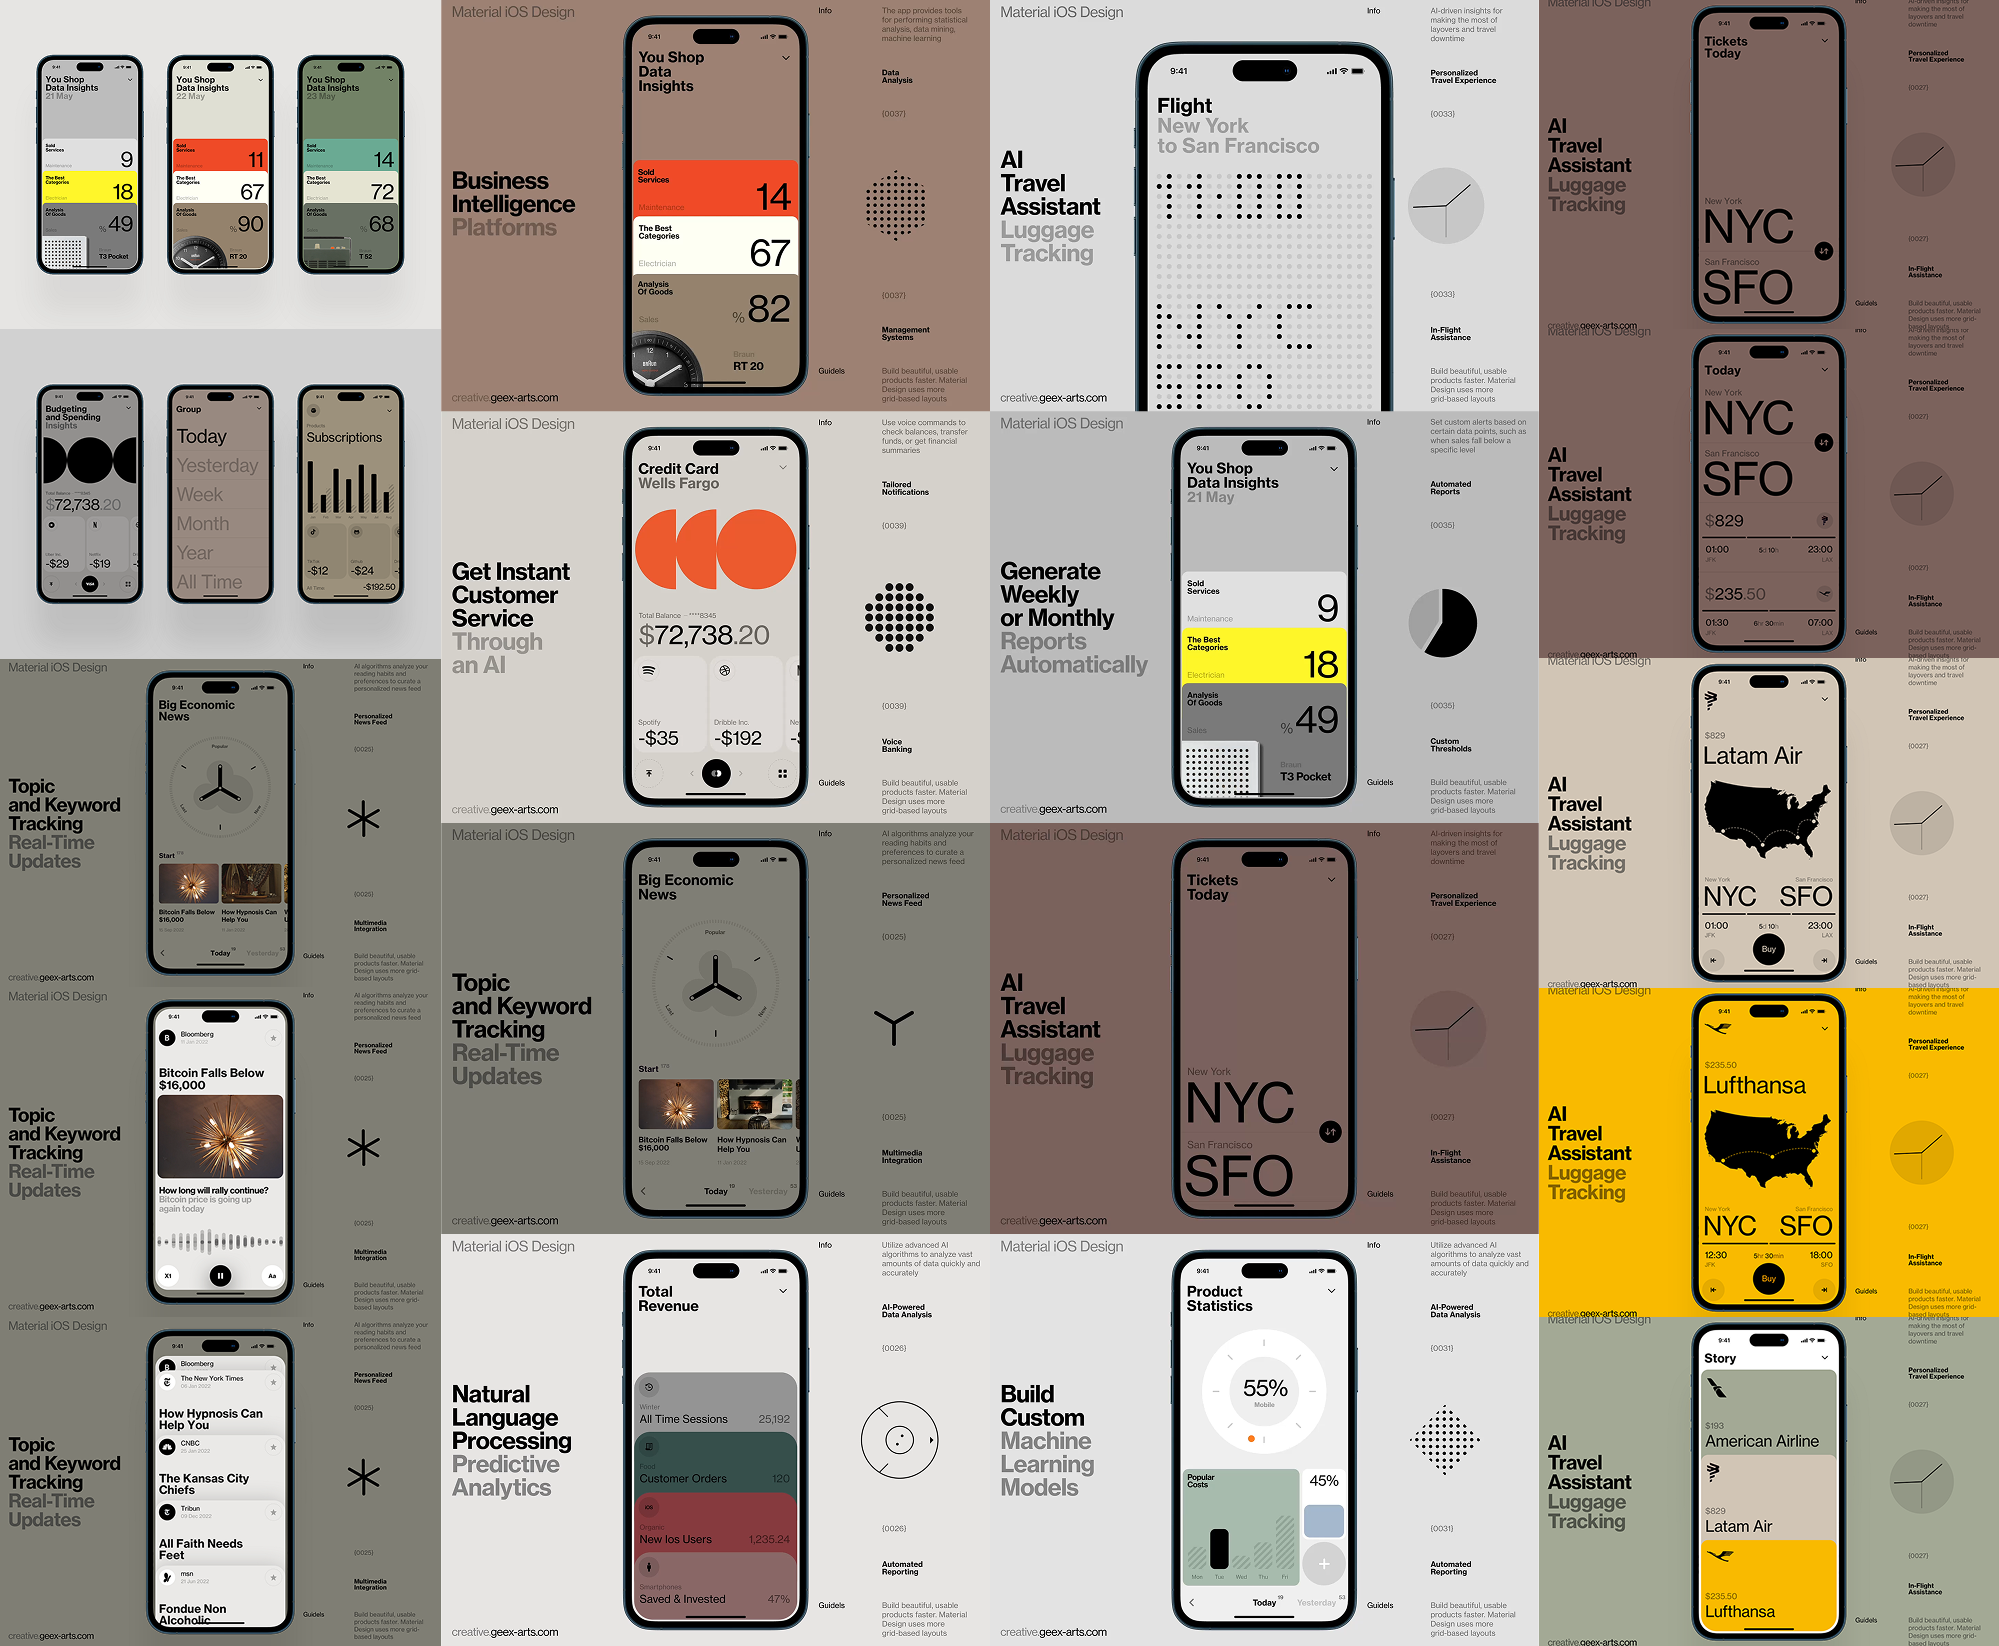
\includegraphics[width=1\textwidth]{foto/swiss_design}
    \caption{Esempio di Swiss Design che ha ispirato l’interfaccia.}
    \label{fig:swiss_design}
\end{figure}

\vspace{\baselineskip}

Un altro aspetto chiave dell'ispirazione proviene dalle esperienze utente
offerte da applicazioni di riferimento come \textbf{Spotify} e
l’\textbf{Orologio di Google}.
In particolare:
\begin{itemize}
    \item Da \textbf{Spotify}, l'app riprende il sistema di navigazione fluido e
    l'uso strategico della tipografia BOLD per evidenziare informazioni
    cruciali.
    \item Dall’\textbf{Orologio di Google}, trae ispirazione per le interazioni
    minimali e intuitive, con transizioni morbide e un focus su un design
    essenziale.
\end{itemize}

\vspace{\baselineskip}

\noindent Di seguito alcuni riferimenti visivi che hanno guidato il processo di
design:

\begin{figure}[H]
    \centering
    \begin{minipage}{0.24\textwidth}
        \centering
        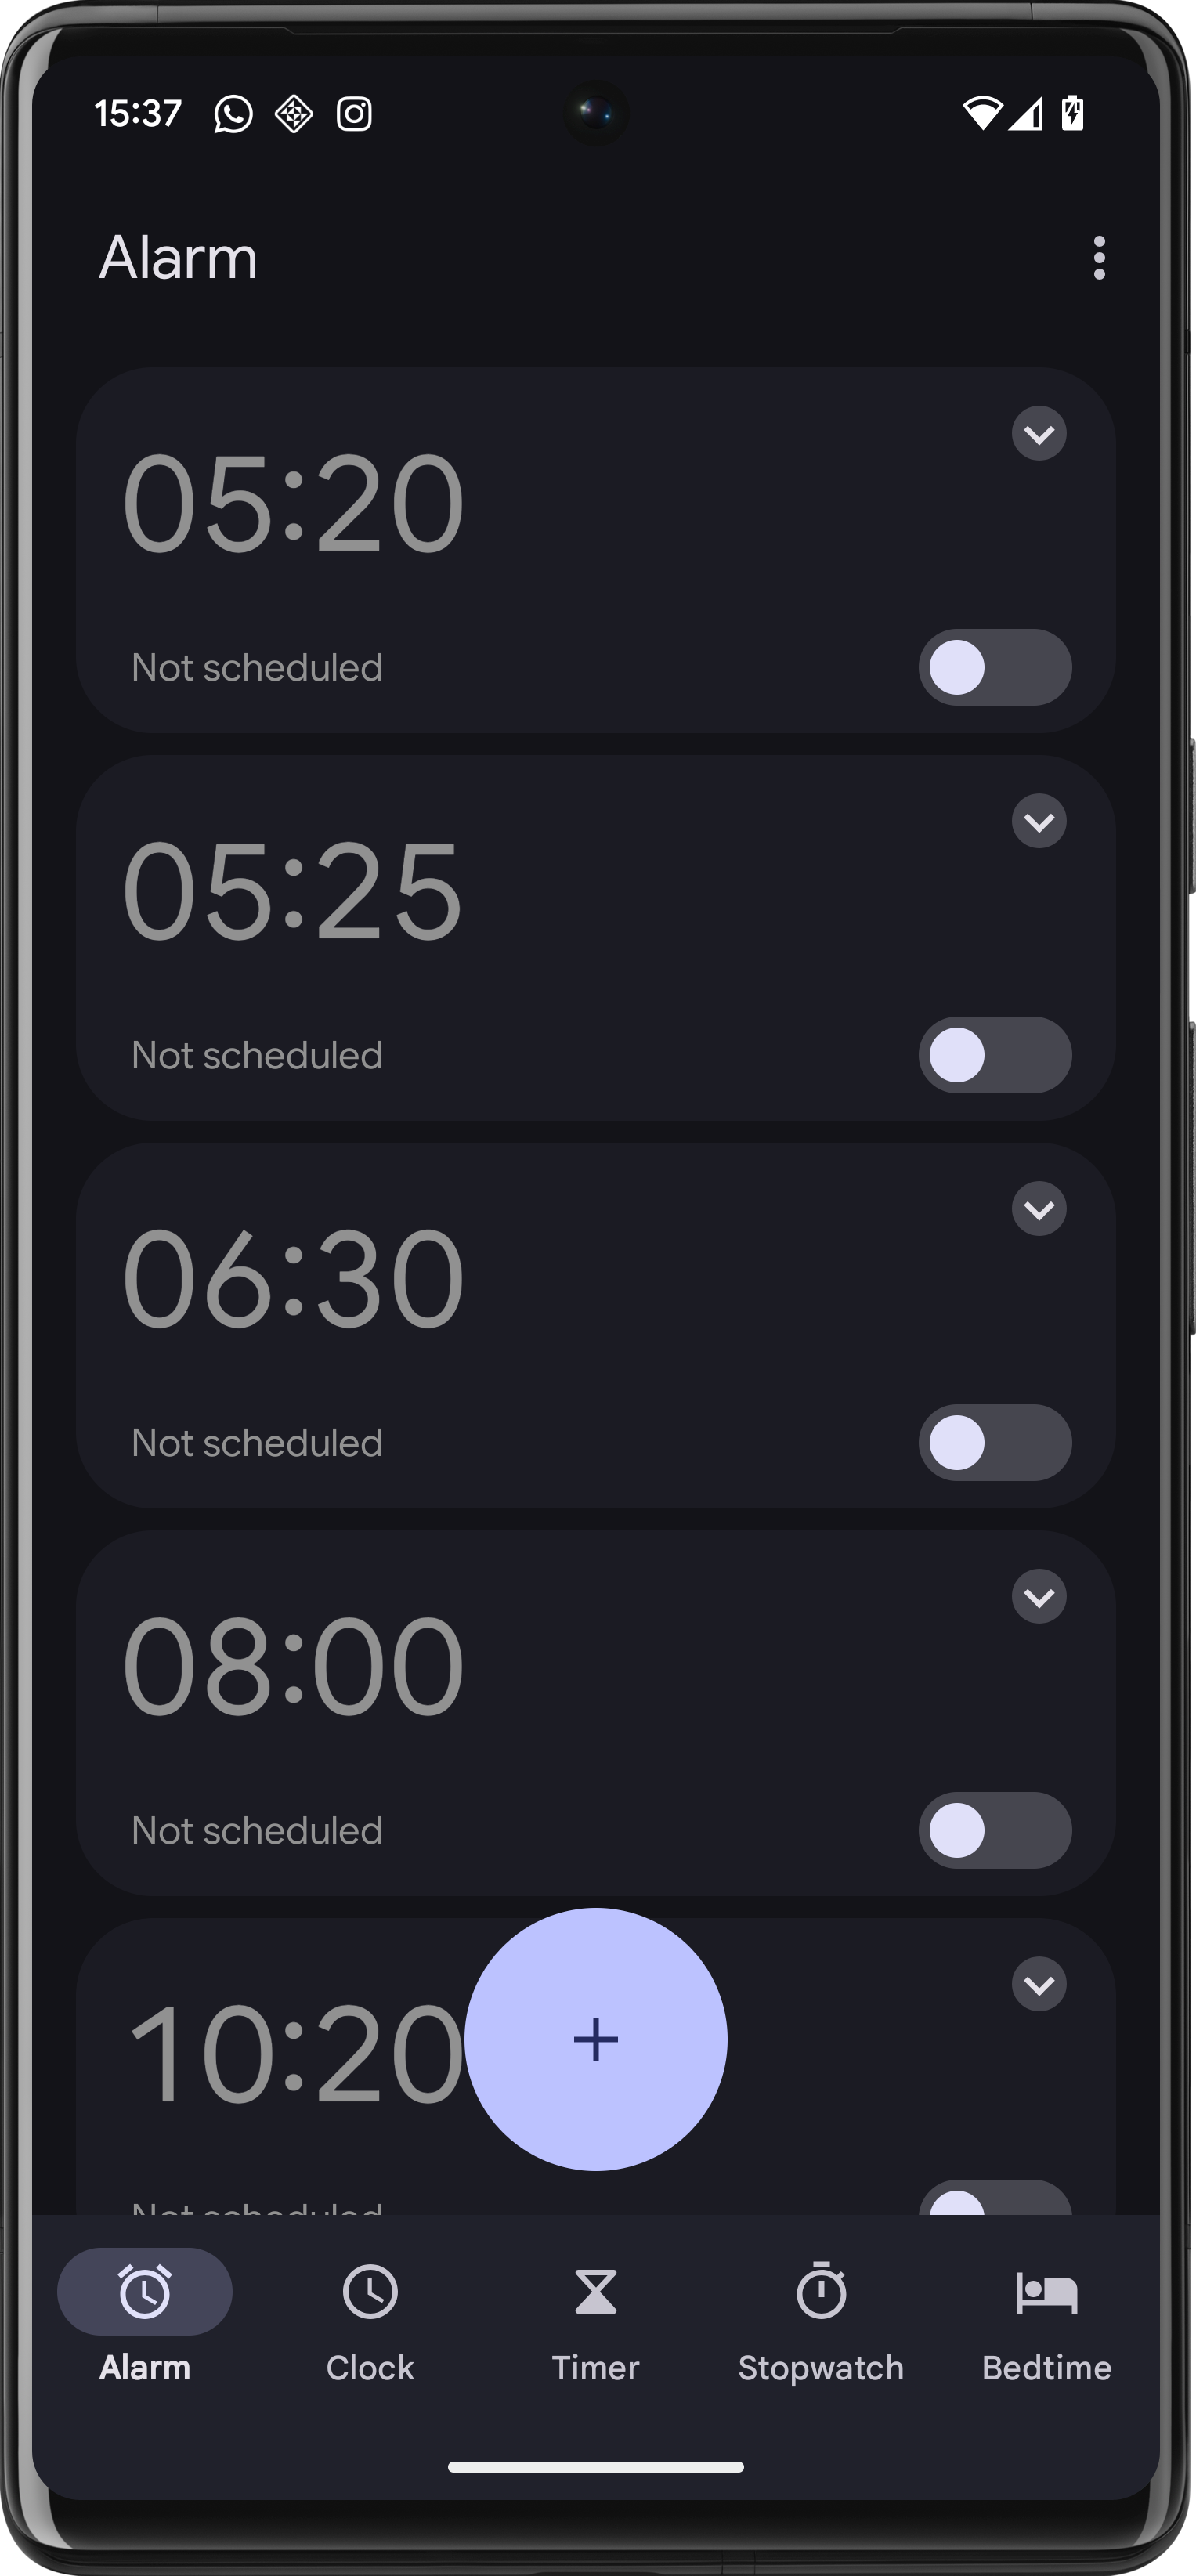
\includegraphics[width=\textwidth]{foto/google_clock_app}
        \label{fig:google_clock}
    \end{minipage}
    \hfill
    \begin{minipage}{0.24\textwidth}
        \centering
        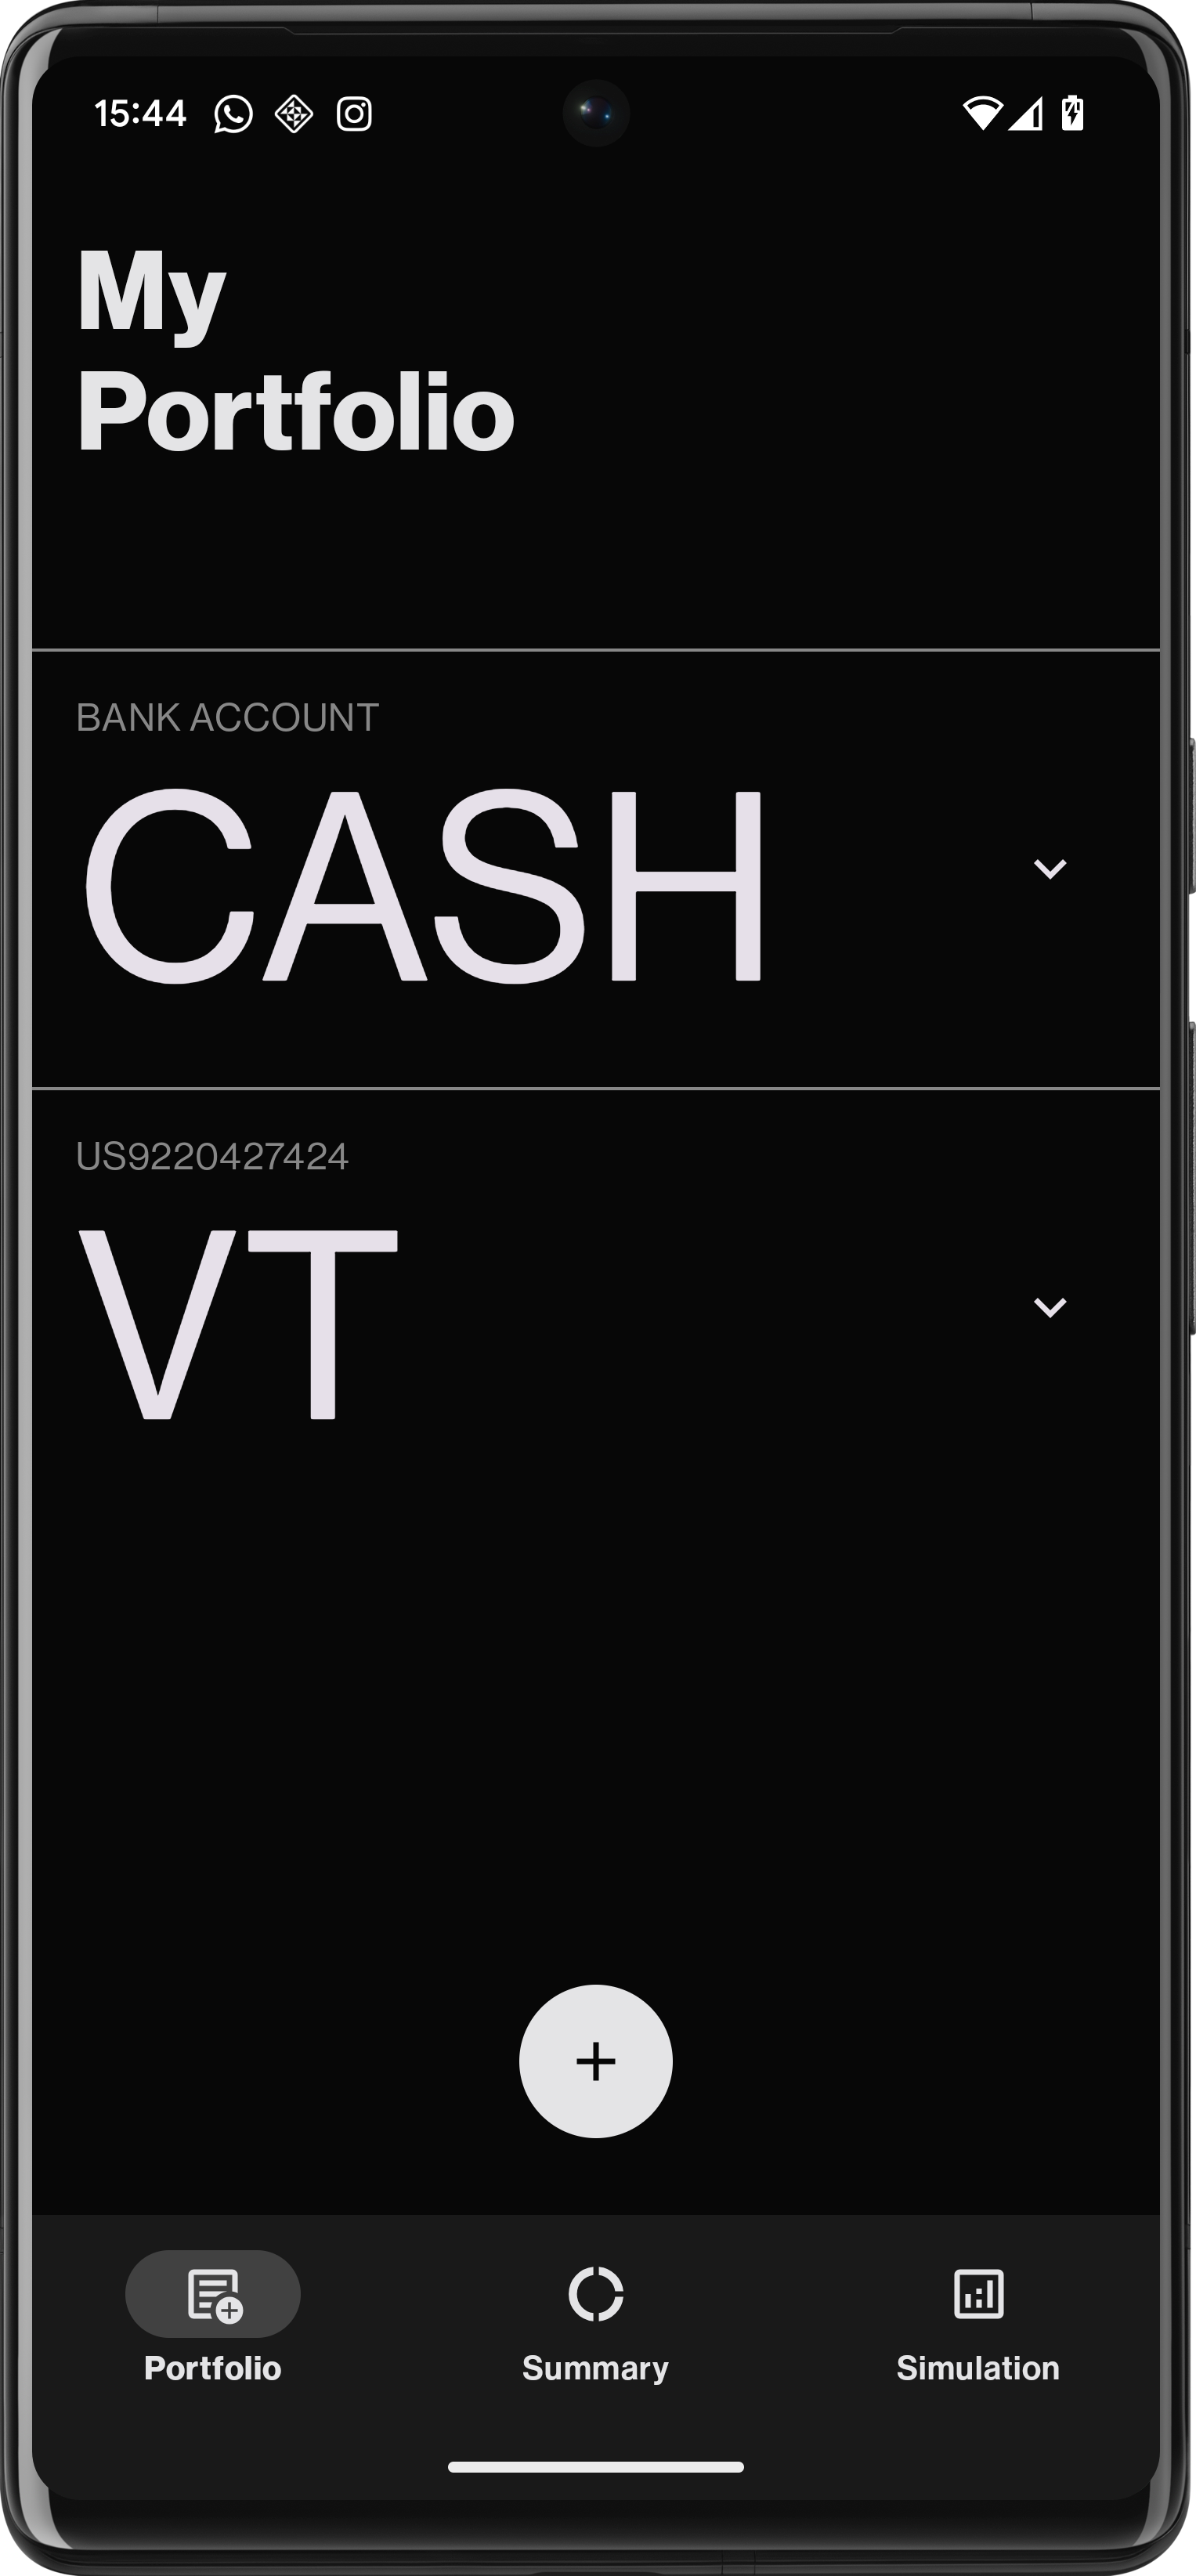
\includegraphics[width=\textwidth]{foto/portfolio_screen}
        \label{fig:portfolio_screen}
    \end{minipage}
    \hfill
    \begin{minipage}{0.24\textwidth}
        \centering
        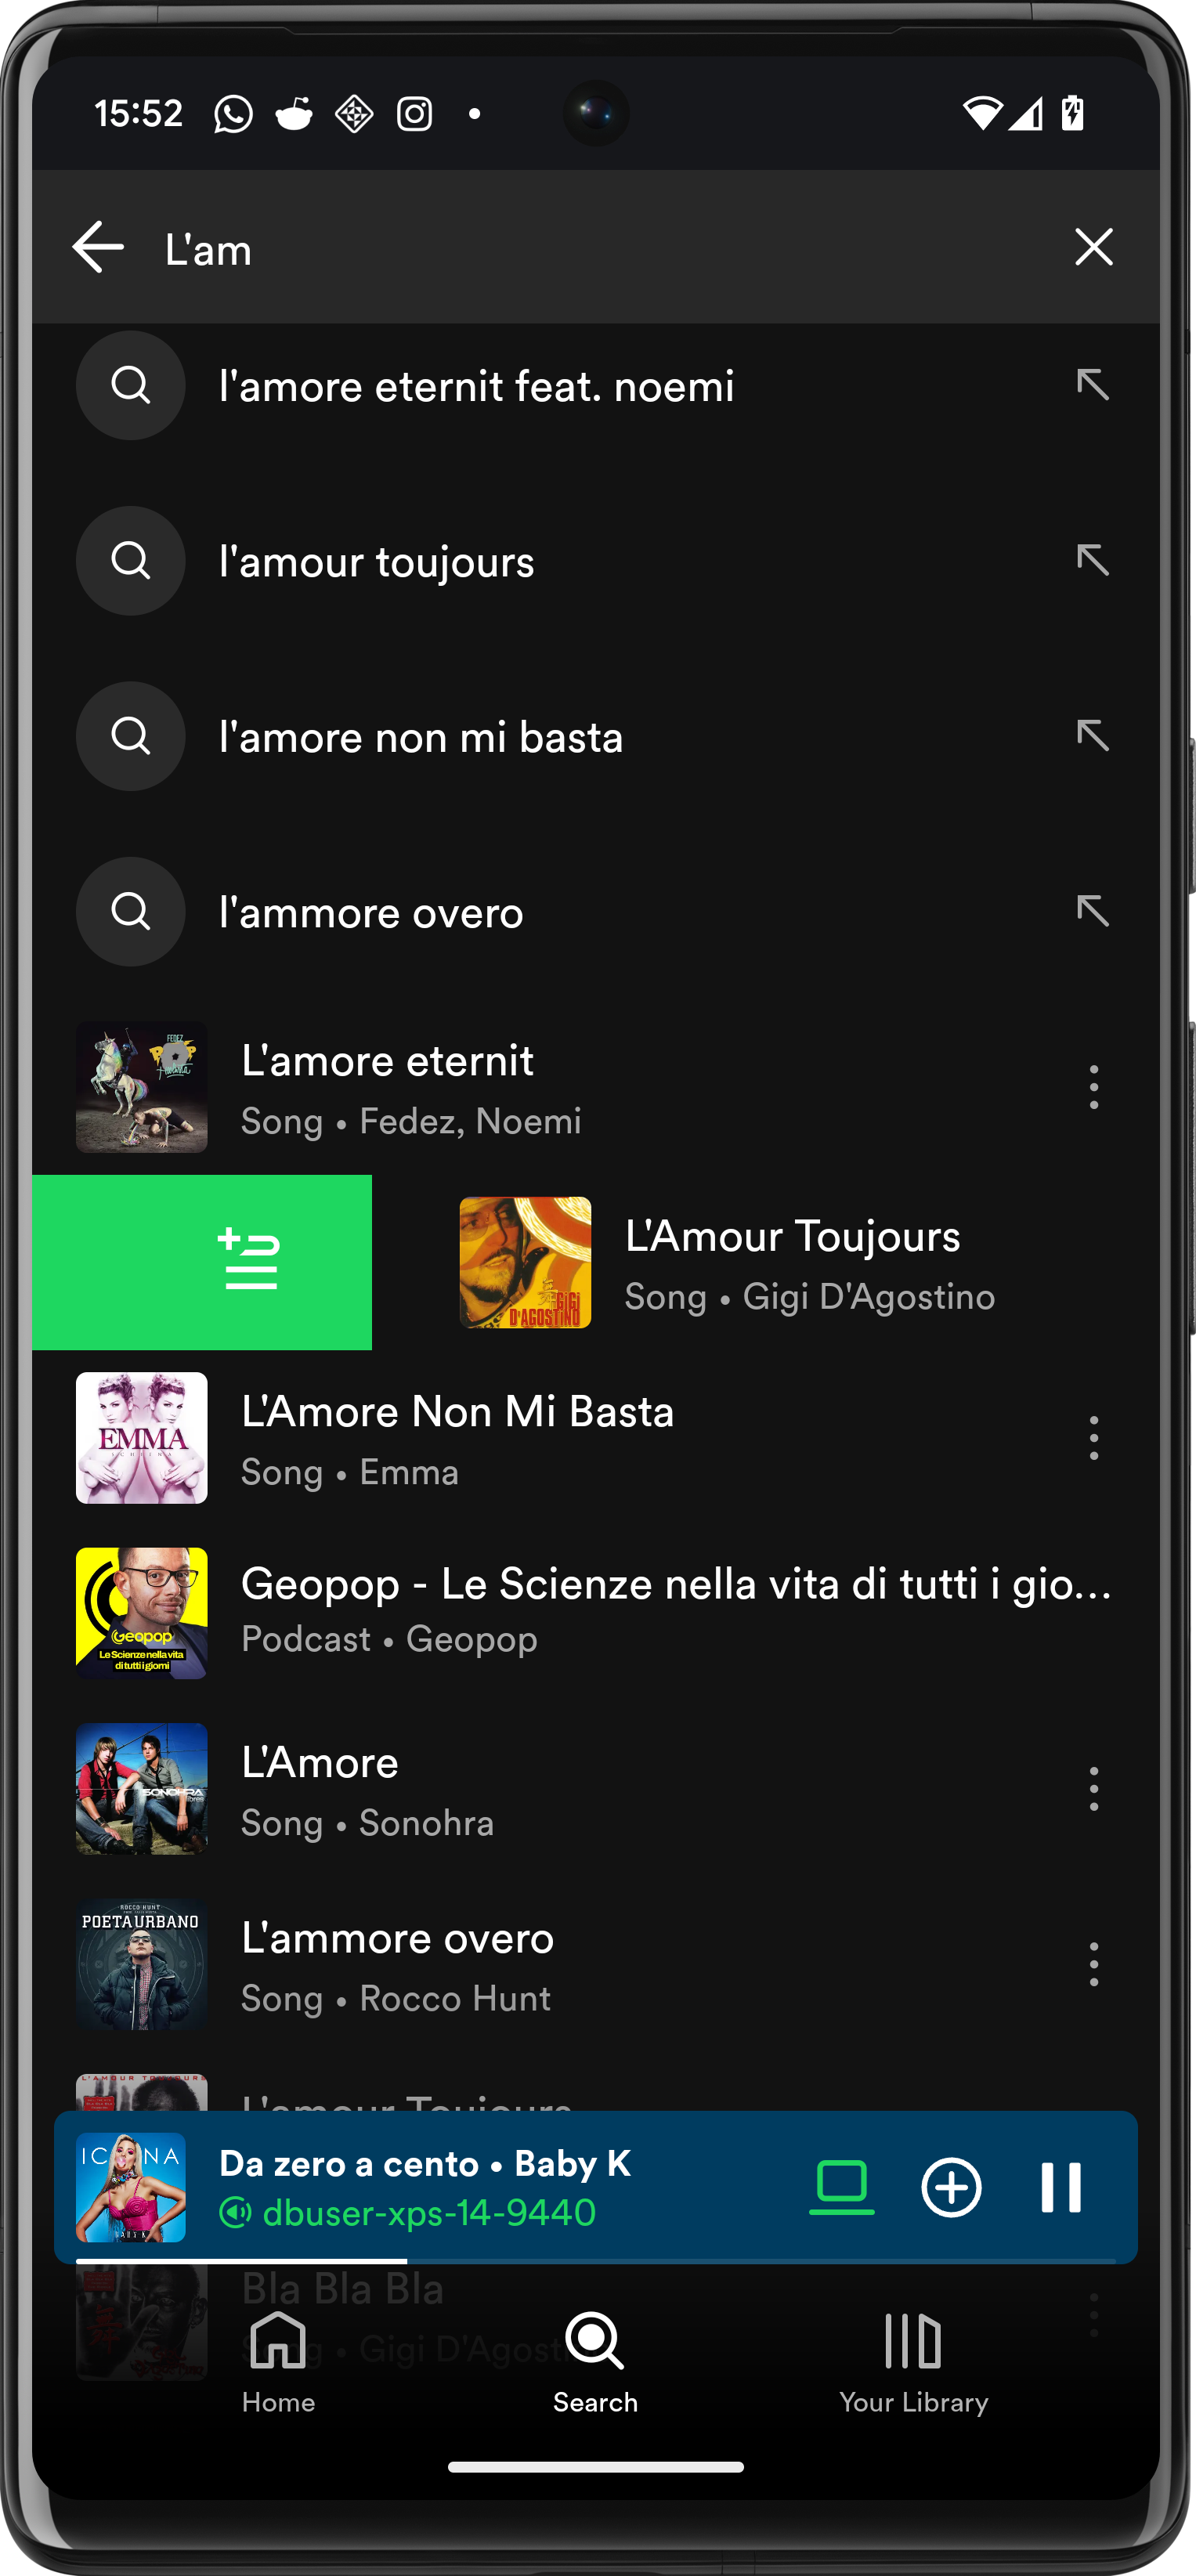
\includegraphics[width=\textwidth]{foto/swipe_interaction_spotify}
        \label{fig:spotify_swipe}
    \end{minipage}
    \hfill
    \begin{minipage}{0.24\textwidth}
        \centering
        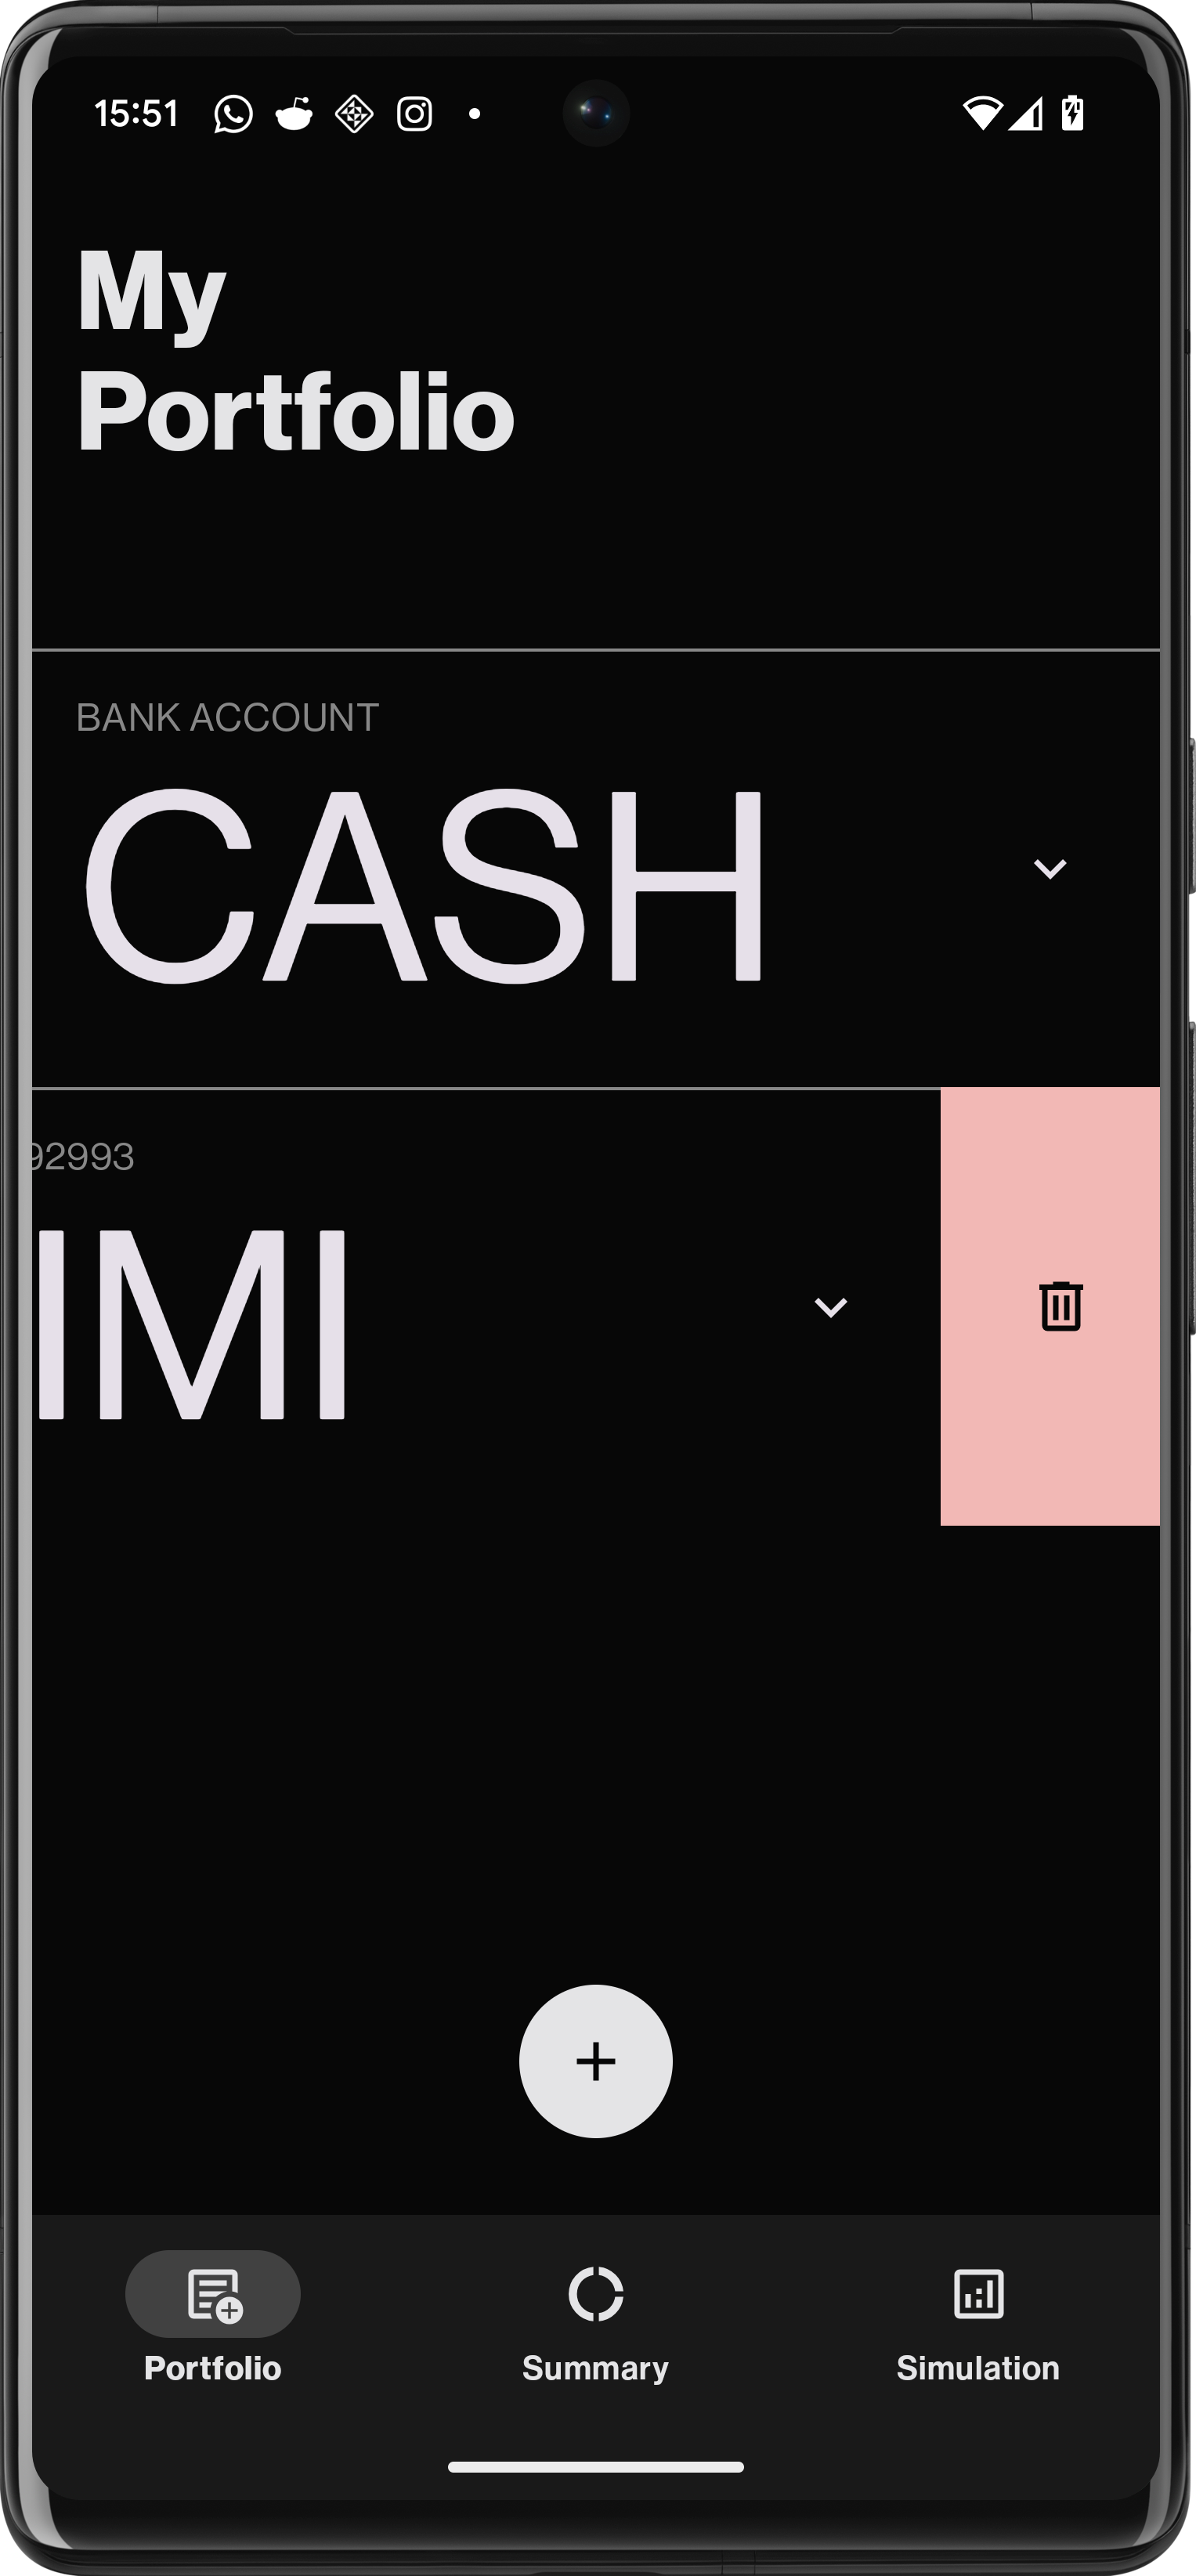
\includegraphics[width=\textwidth]{foto/swipe_interaction}
        \label{fig:swipe_delete}
    \end{minipage}
\end{figure}

\definecolor{light1}{HTML}{19191B}
\definecolor{light2}{HTML}{787878}
\definecolor{light3}{HTML}{F8F8F8}
\definecolor{light4}{HTML}{E6E6E6}
\definecolor{light5}{HTML}{BEBEBE}
\definecolor{light6}{HTML}{E1E1E1}
\definecolor{light7}{HTML}{8E8E8E}

\definecolor{dark1}{HTML}{E4E4E6}
\definecolor{dark2}{HTML}{878787}
\definecolor{dark3}{HTML}{070707}
\definecolor{dark4}{HTML}{191919}
\definecolor{dark5}{HTML}{414141}
\definecolor{dark6}{HTML}{1E1E1E}
\definecolor{dark7}{HTML}{717171}

\section{Colori e Tipografia}\label{sec:colori_tipografia}
Il sistema cromatico di \textbf{IgnitionFinance} è progettato per garantire massima leggibilità e flessibilità tra tema chiaro e scuro.
L'interfaccia utilizza una scala di grigi, dal nero assoluto al bianco puro, per mantenere un aspetto serio e professionale.

\vspace{\baselineskip}

\noindent Di seguito vengono mostrati i colori utilizzati per entrambi i temi:

\begin{figure}[H]
    \centering
    \begin{subfigure}[b]{\textwidth}
        \centering
        \foreach \colorname in {light1, light2, light3, light4, light5, light6, light7} {
            \begin{minipage}{0.12\textwidth}
                \centering
                \colorbox{\colorname}{{\color{\colorname}\rule{2cm}{2cm}}}
            \end{minipage}
            \hfill
        }
        \caption{Palette colori per il tema chiaro.}
        \label{fig:palette_light}
    \end{subfigure}

    \vspace{0.5cm}

    \begin{subfigure}[b]{\textwidth}
        \centering
        \foreach \colorname in {dark1, dark2, dark3, dark4, dark5, dark6, dark7} {
            \begin{minipage}{0.12\textwidth}
                \centering
                \colorbox{\colorname}{{\color{\colorname}\rule{2cm}{2cm}}}
            \end{minipage}
            \hfill
        }
        \caption{Palette colori per il tema scuro.}
        \label{fig:palette_dark}
    \end{subfigure}

    \label{fig:palette_all}
\end{figure}

\noindent La tipografia adottata per \textbf{IgnitionFinance} si basa su \textbf{Neue Haas Grotesk Display Pro}, una rivisitazione digitale della celebre Haas Grotesk, un font sans-serif sviluppato originariamente nel 1957 da Max Miedinger ed Eduard Hoffmann presso la fonderia Haas in Svizzera.
Inizialmente noto come Haas Grotesk, il carattere venne ribattezzato Helvetica nel 1960, evidenziando così le sue radici svizzere e la sua adozione globale.

\noindent Nel contesto del design moderno, e per rispondere alle esigenze digitali, nel 2010 fu realizzata una versione rivisitata, \textbf{Neue Haas Grotesk Display Pro}, che si propone di mantenere l'estetica pulita e la funzionalità del design svizzero.
Questa versione offre diverse varianti, ciascuna studiata per specifiche funzioni comunicative:
\begin{itemize}
    \item \textbf{Regular}: Ideale per il testo principale, garantisce leggibilità e una presentazione sobria.
    \item \textbf{Medium}: Utilizzato per enfatizzare elementi importanti, offrendo un giusto equilibrio tra sobrietà ed evidenza.
    \item \textbf{Bold}: Perfetto per titoli e sottotitoli, crea una chiara gerarchia visiva e attira l'attenzione.
\end{itemize}

\noindent Questo font viene utilizzato non solo nell'interfaccia di \textbf{IgnitionFinance}, ma anche in tutta la documentazione, garantendo così coerenza e un'identità visiva riconoscibile.
La scelta di \textbf{Neue Haas Grotesk Display Pro} sottolinea l'importanza di una comunicazione chiara e professionale, elementi fondamentali per un'esperienza utente di alta qualità.

\vspace{\baselineskip}

\begin{figure}[H]
    \centering
    \begin{minipage}{0.24\textwidth}
        \centering
        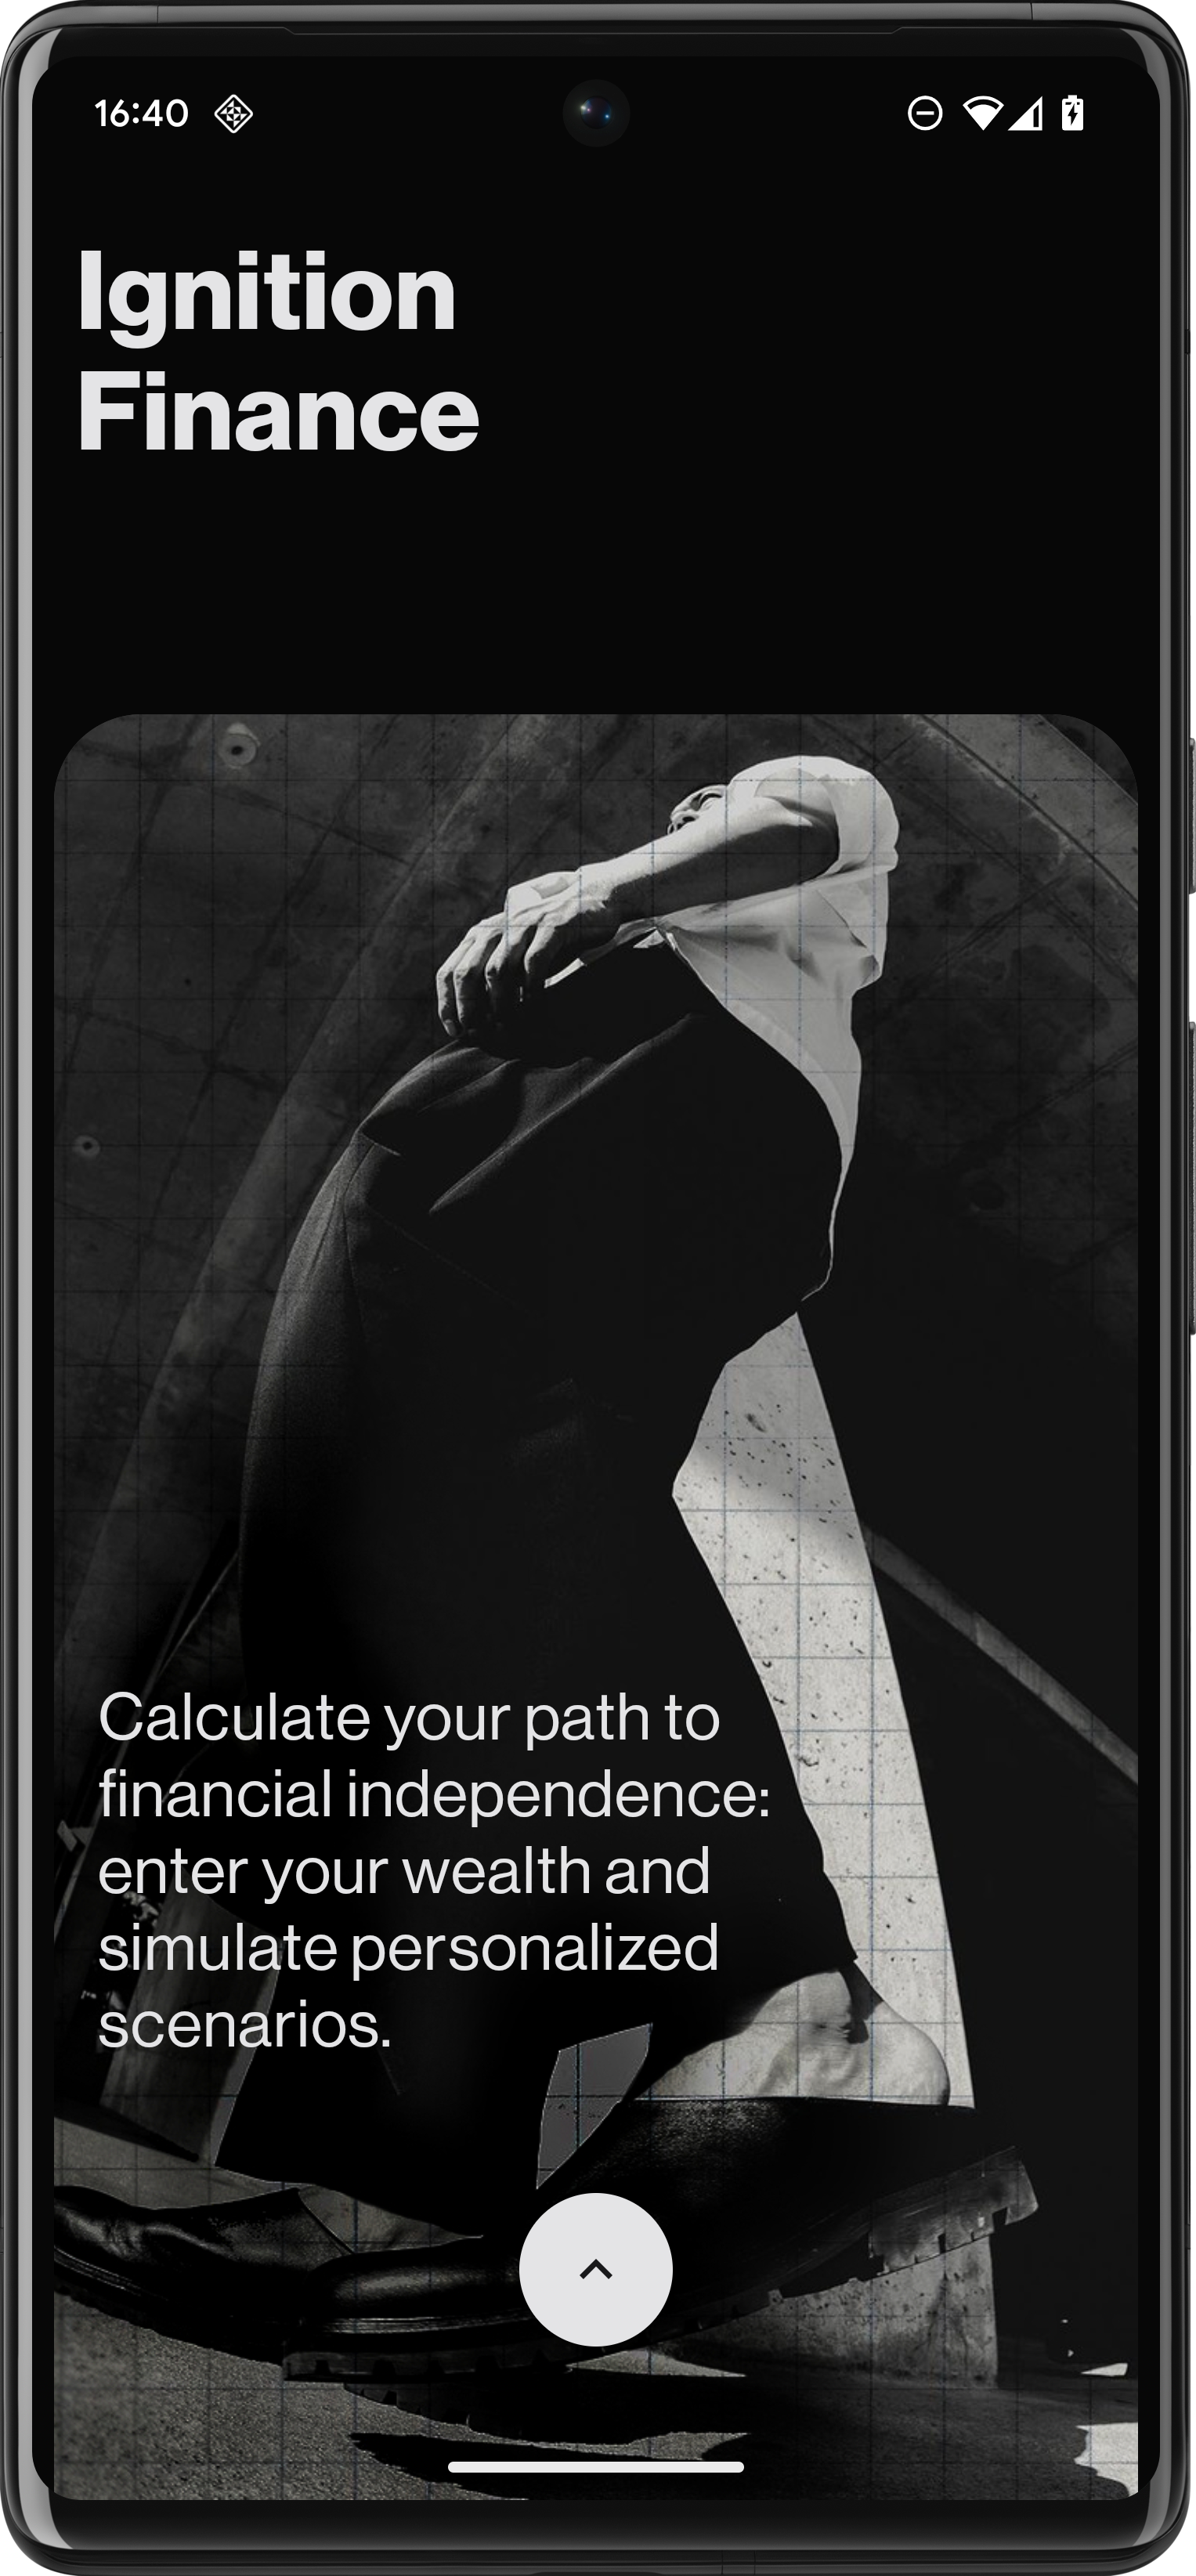
\includegraphics[width=\textwidth]{foto/intro_screen}
        \label{fig:intro_screen}
    \end{minipage}
    \hfill
    \begin{minipage}{0.24\textwidth}
        \centering
        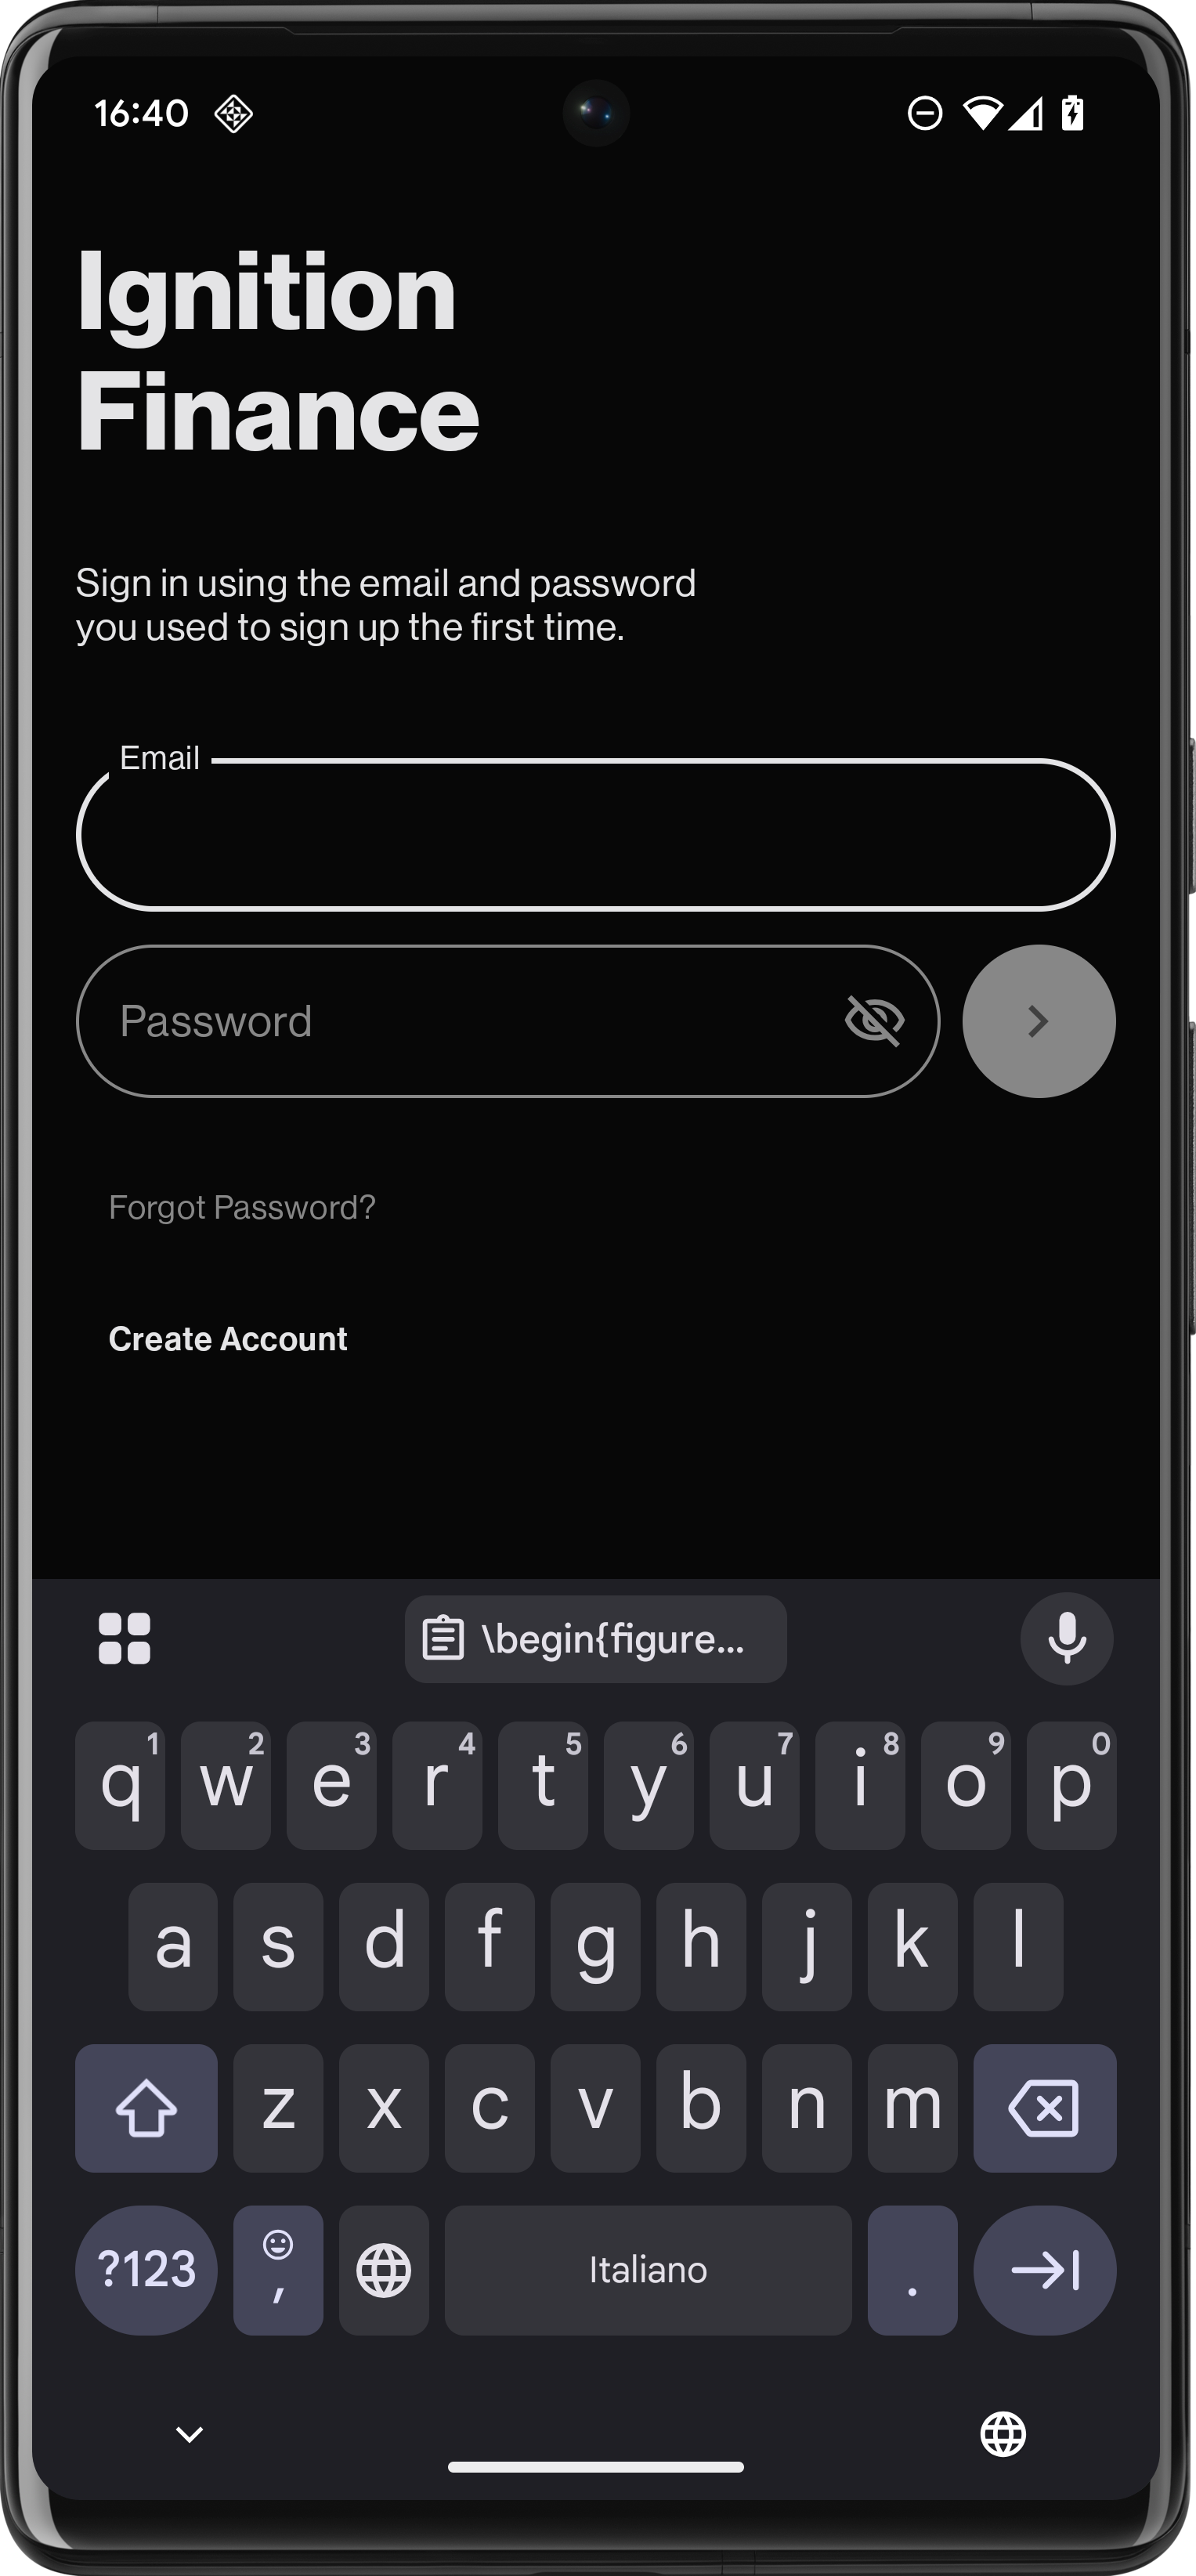
\includegraphics[width=\textwidth]{foto/login}
        \label{fig:login}
    \end{minipage}
    \hfill
    \begin{minipage}{0.24\textwidth}
        \centering
        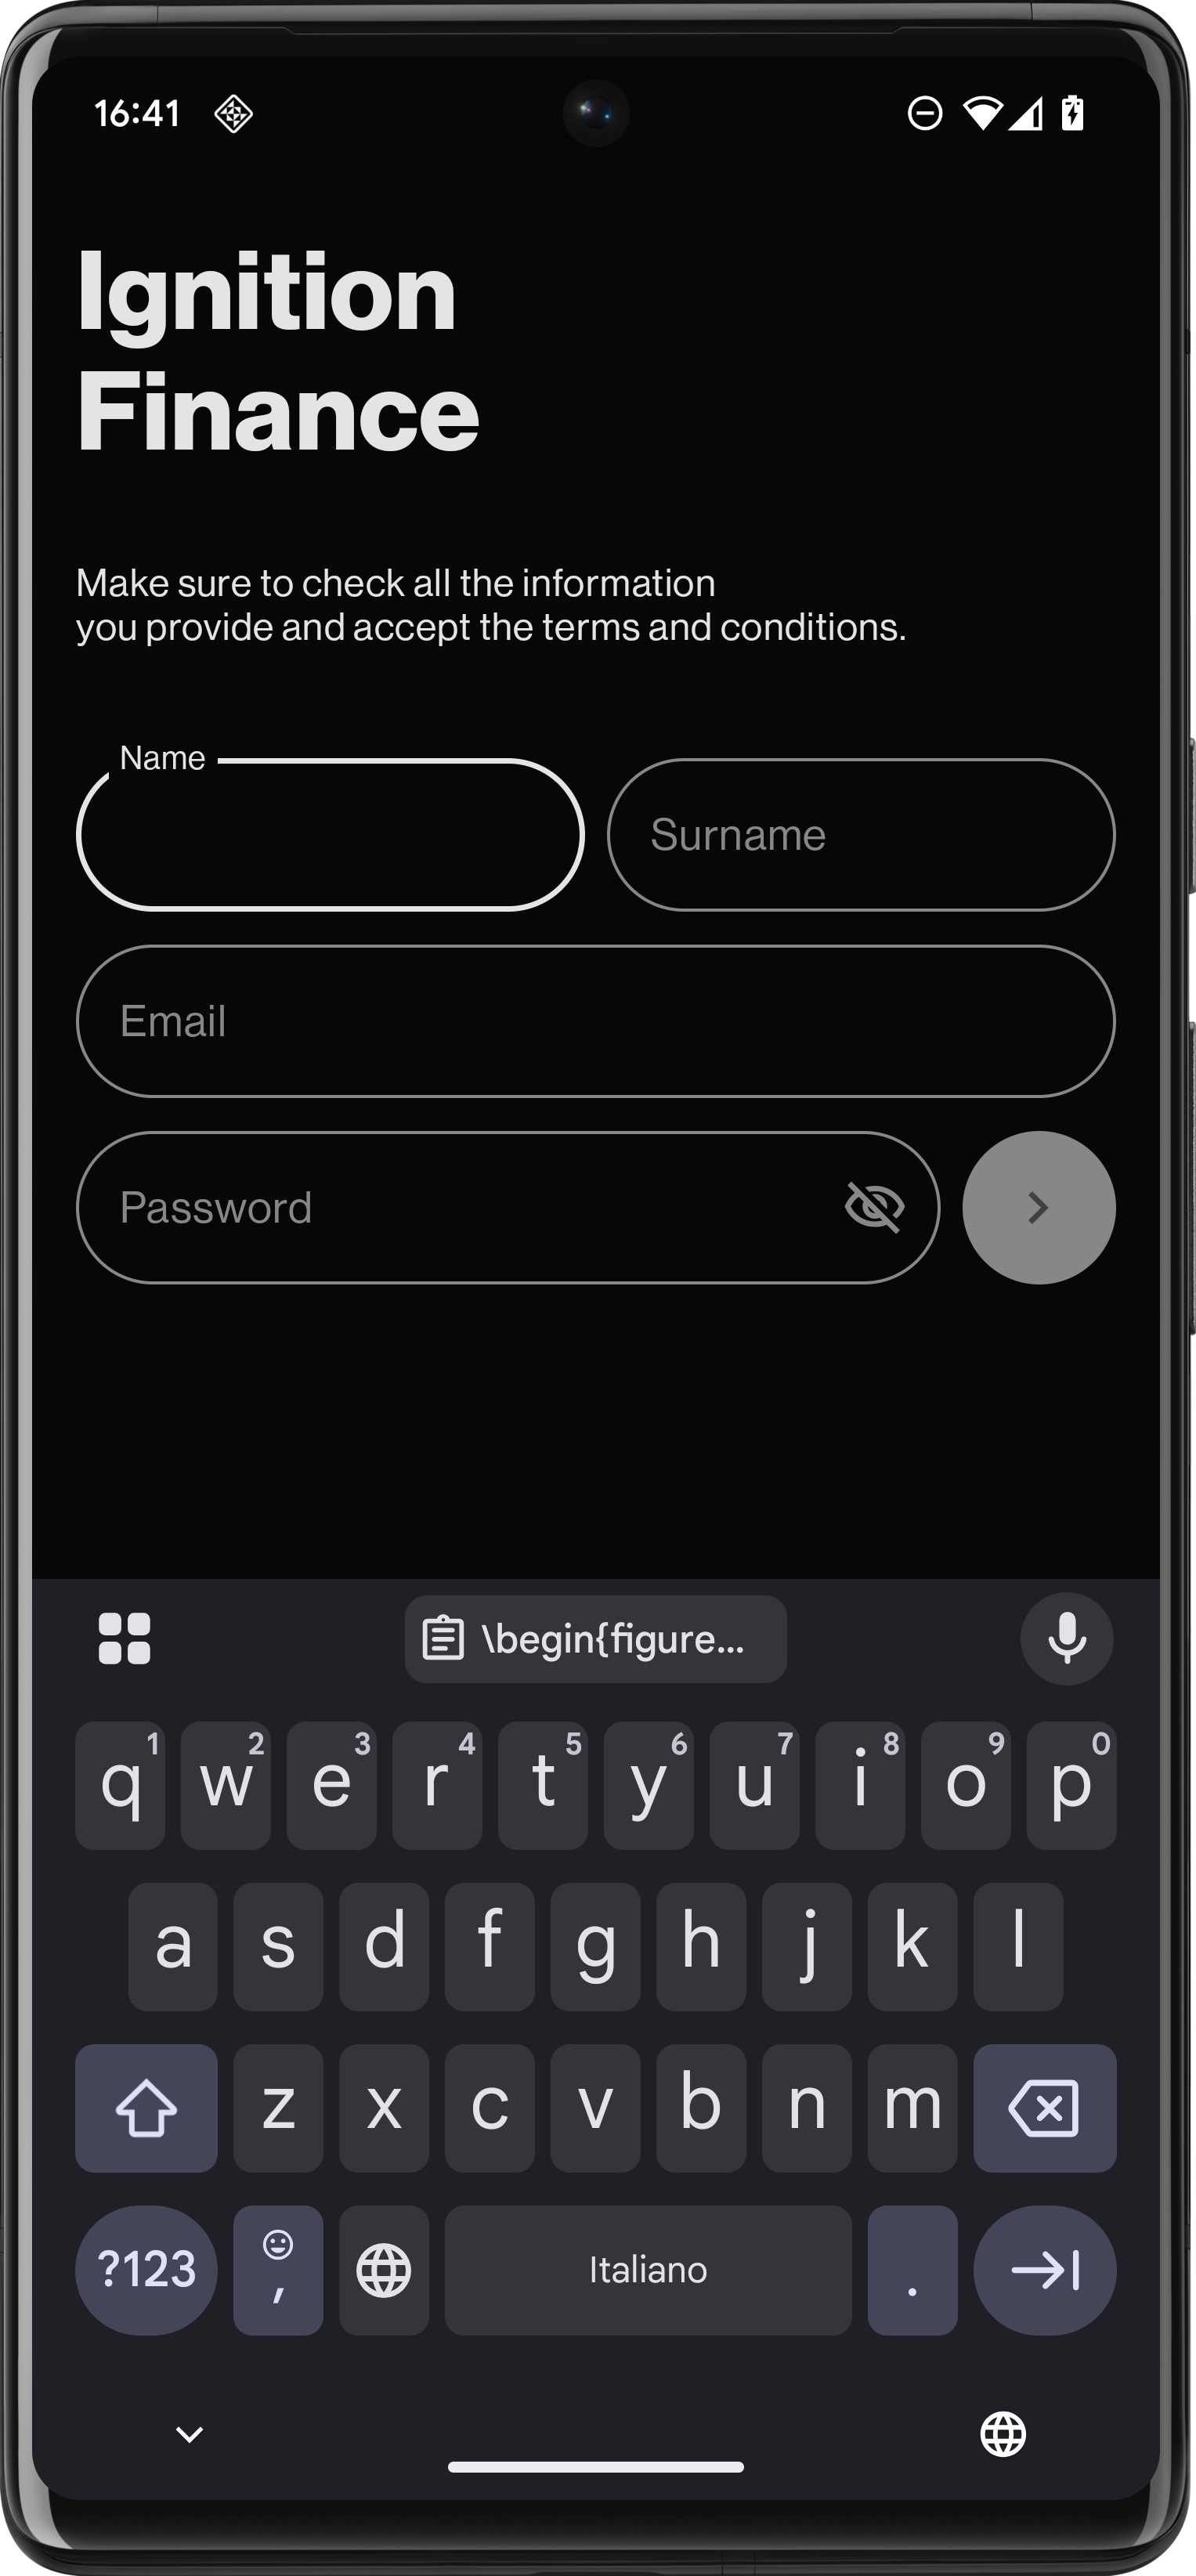
\includegraphics[width=\textwidth]{foto/signup}
        \label{fig:signup}
    \end{minipage}
    \hfill
    \begin{minipage}{0.24\textwidth}
        \centering
        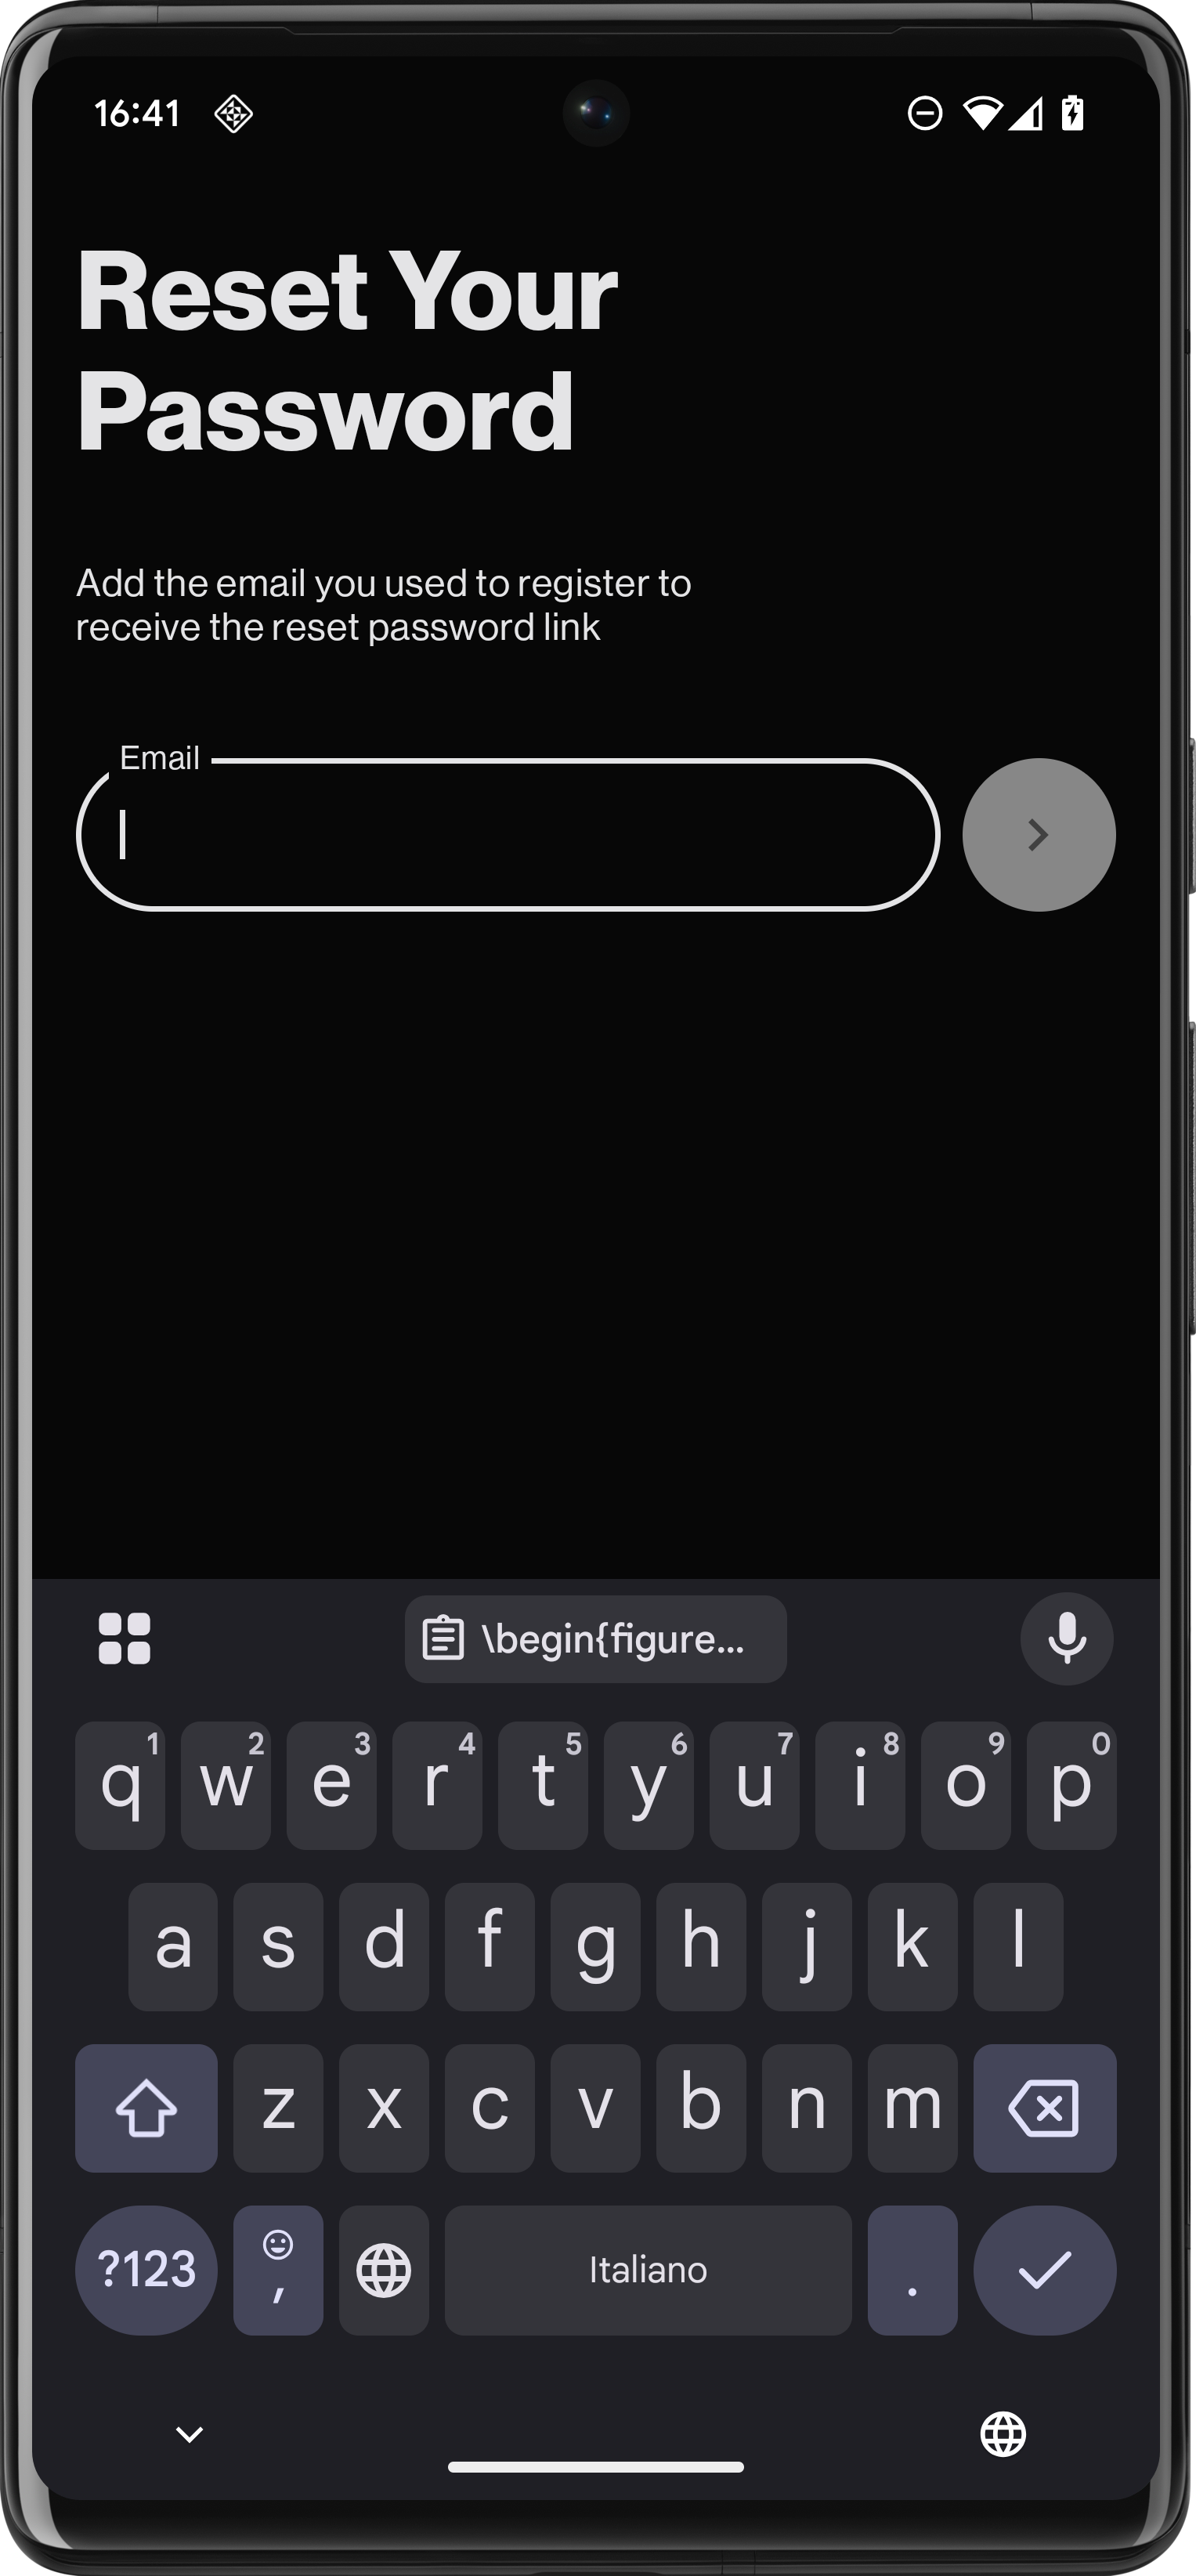
\includegraphics[width=\textwidth]{foto/forgot_password}
        \label{fig:forgot_password}
    \end{minipage}
\end{figure}

\begin{figure}[H]
    \centering
    \begin{minipage}{0.24\textwidth}
        \centering
        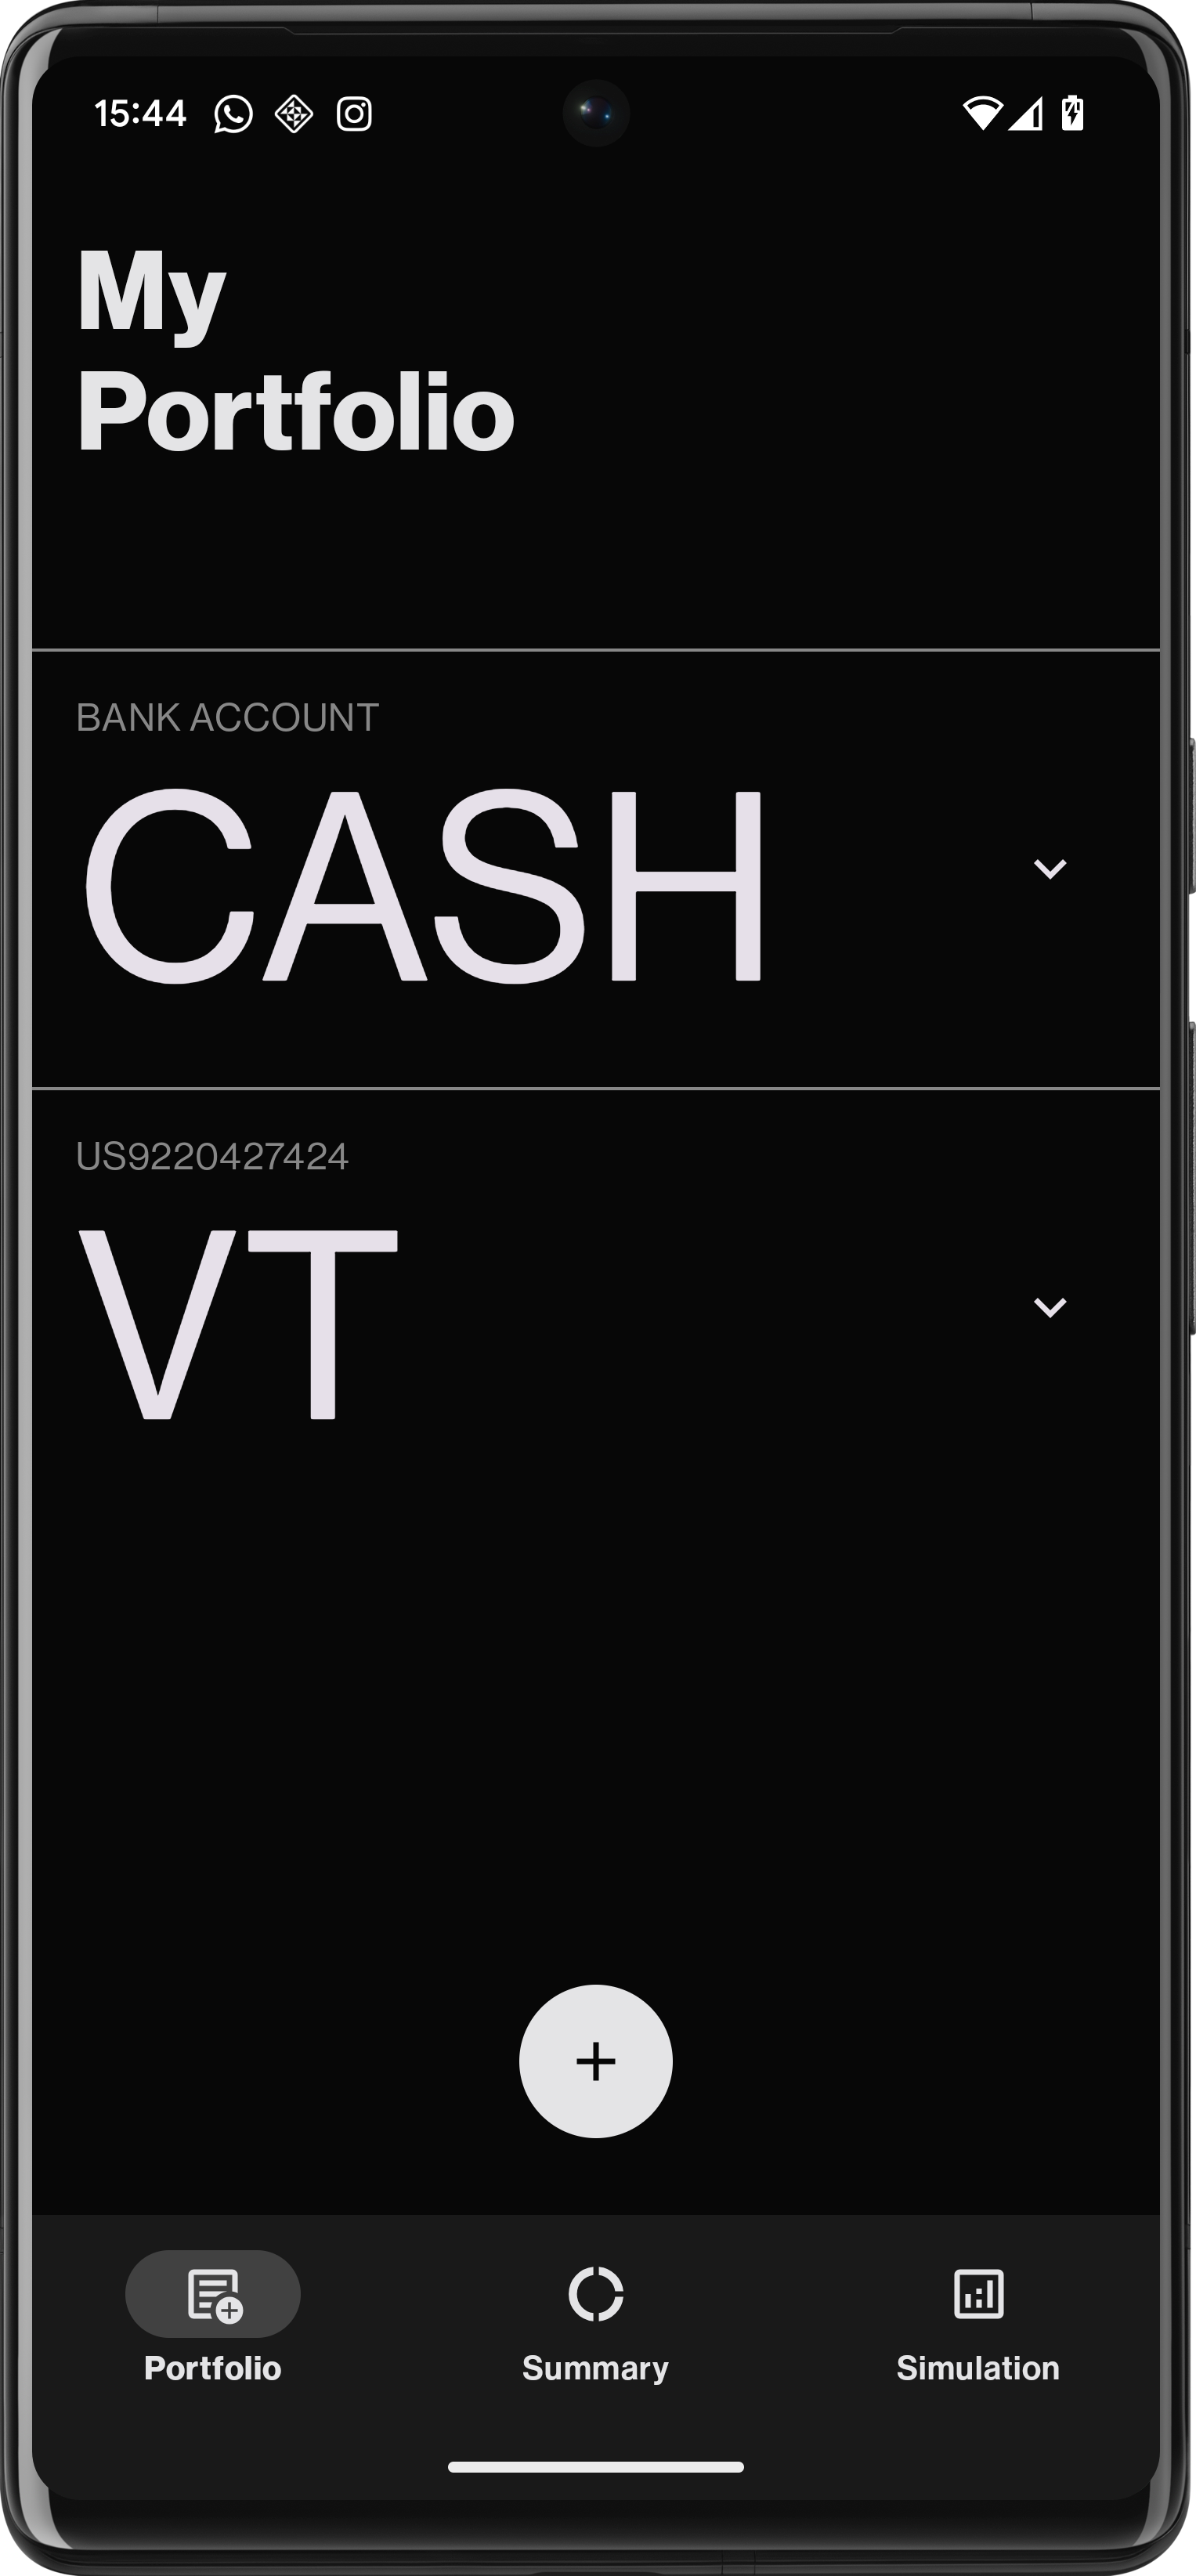
\includegraphics[width=\textwidth]{foto/portfolio_screen}
        \label{fig:portfolio_card}
    \end{minipage}
    \hfill
    \begin{minipage}{0.24\textwidth}
        \centering
        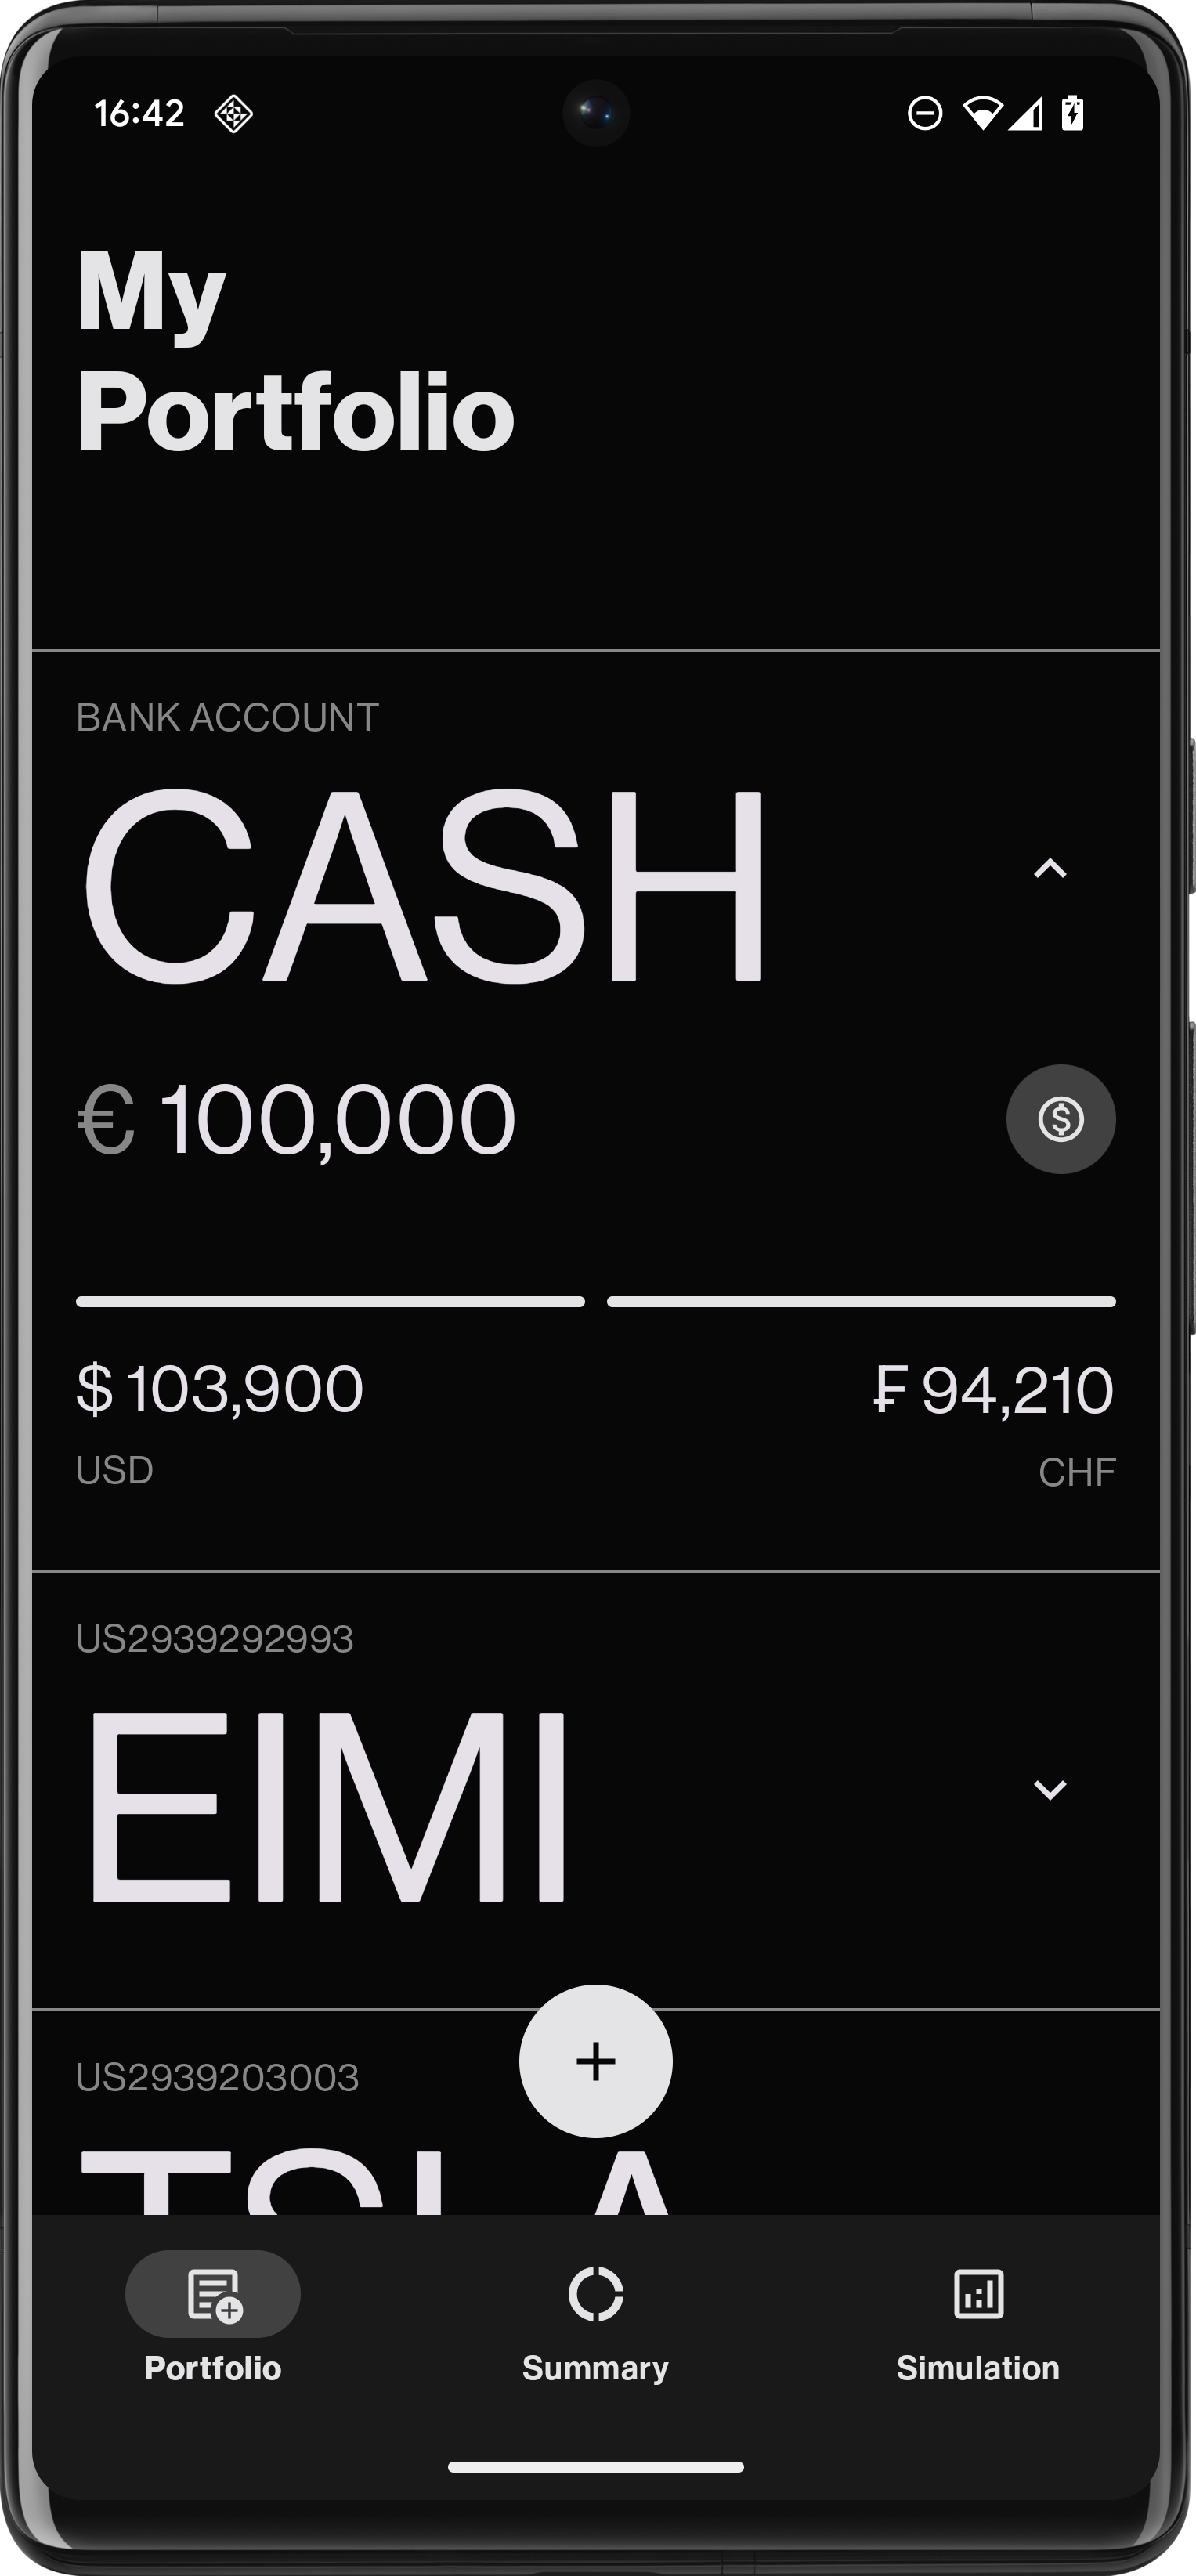
\includegraphics[width=\textwidth]{foto/cash_card}
        \label{fig:cash_card}
    \end{minipage}
    \hfill
    \begin{minipage}{0.24\textwidth}
        \centering
        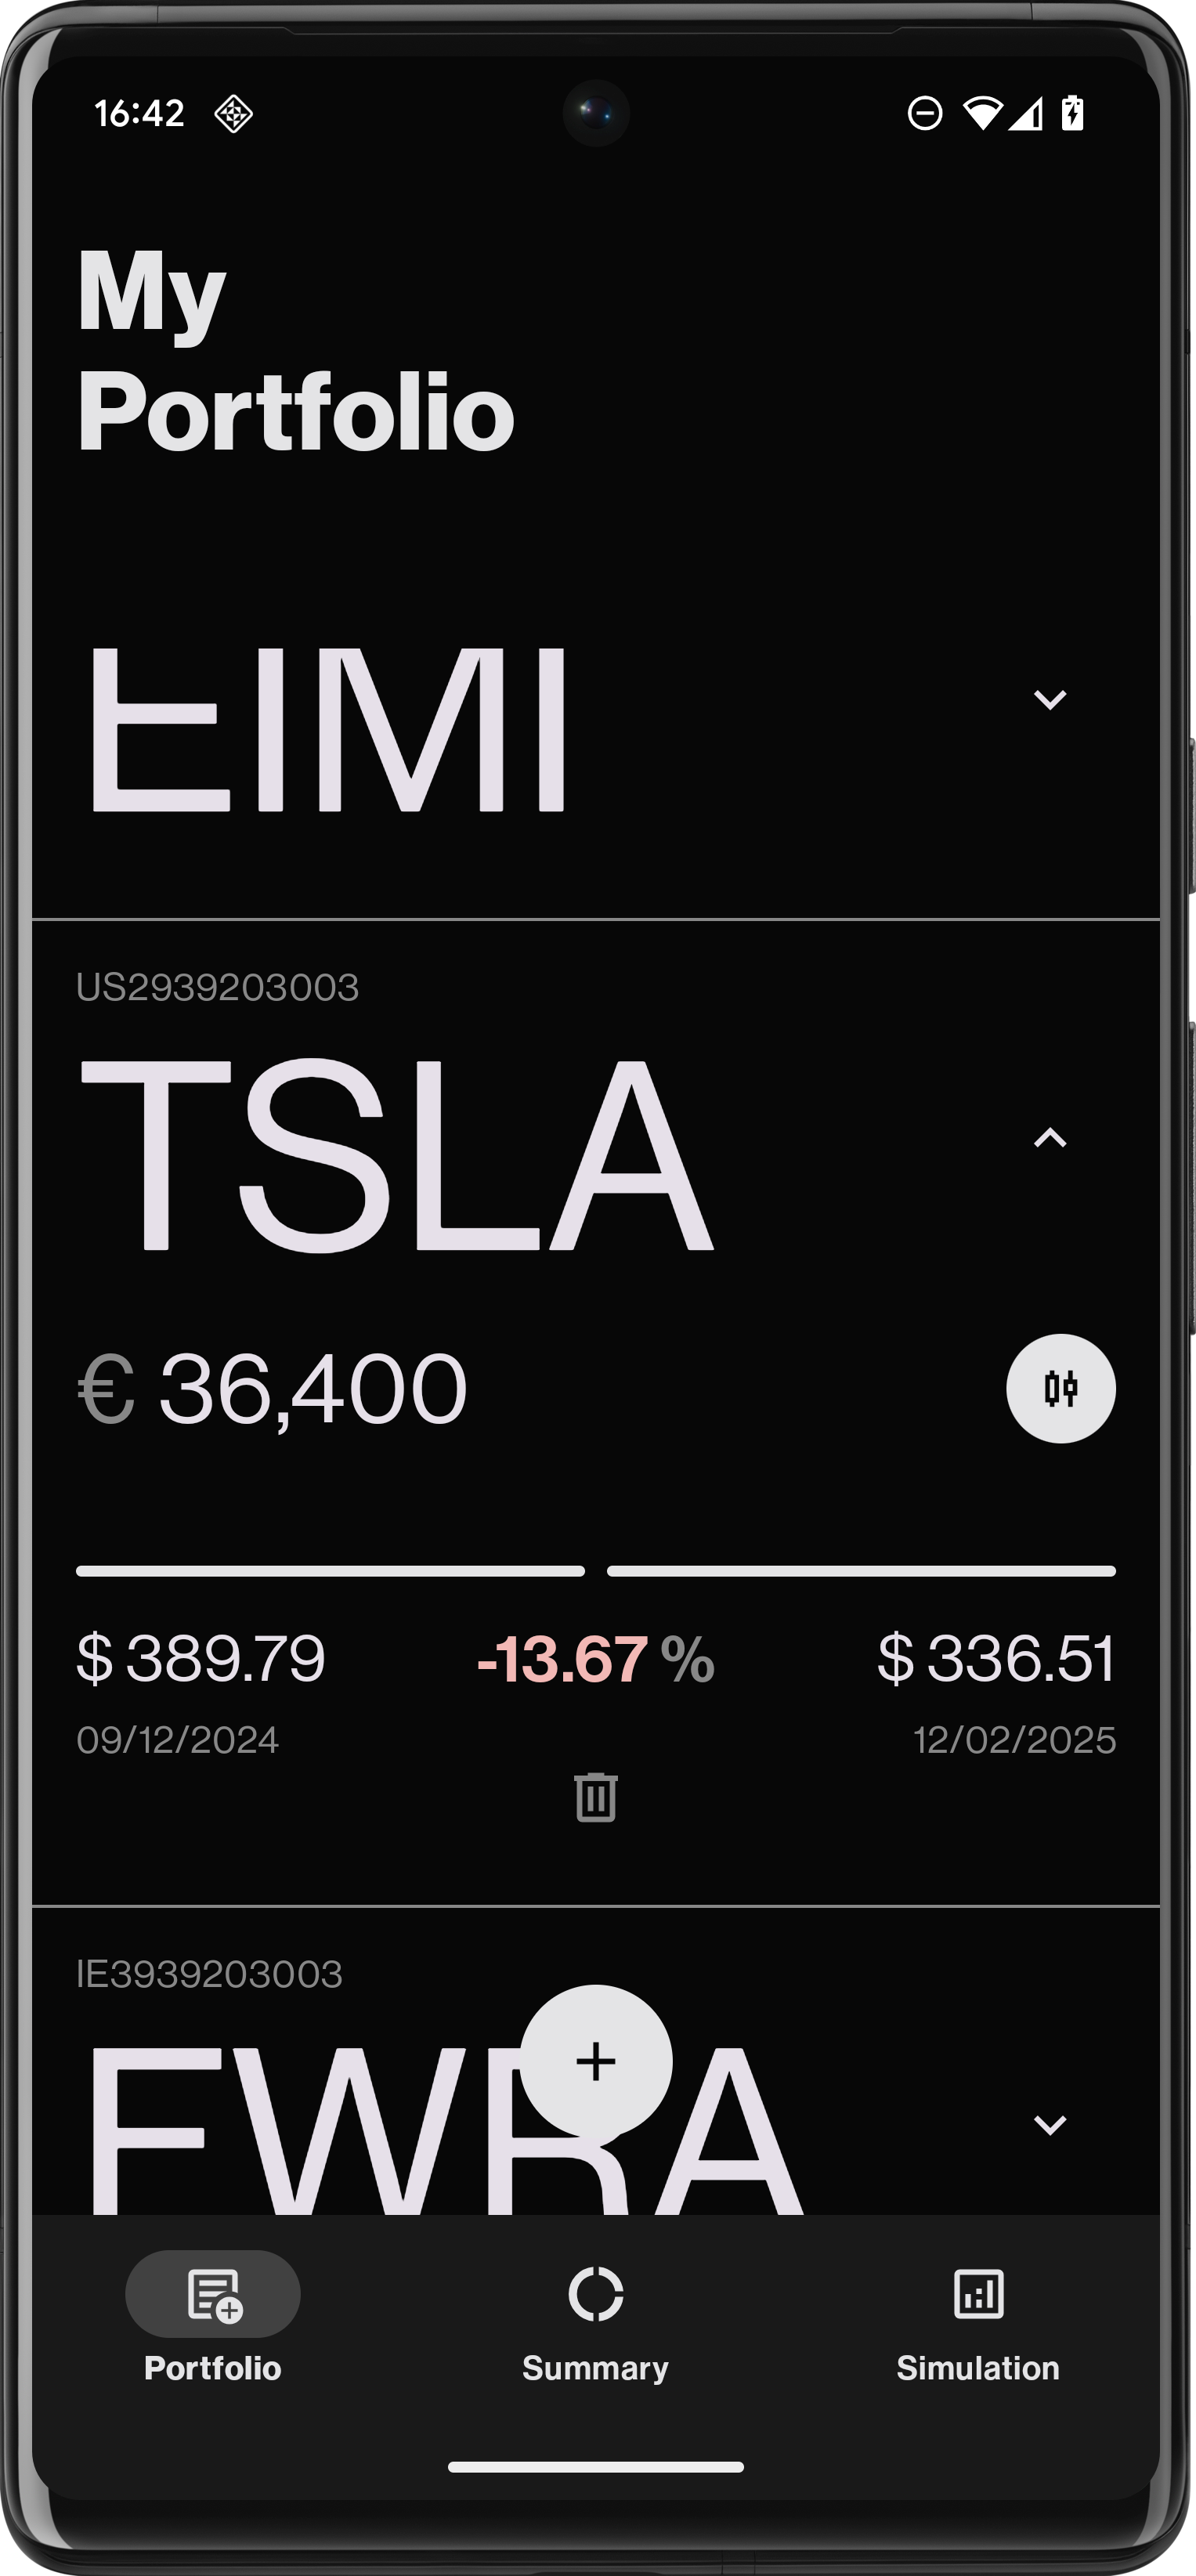
\includegraphics[width=\textwidth]{foto/product_card}
        \label{fig:product_card}
    \end{minipage}
    \hfill
    \begin{minipage}{0.24\textwidth}
        \centering
        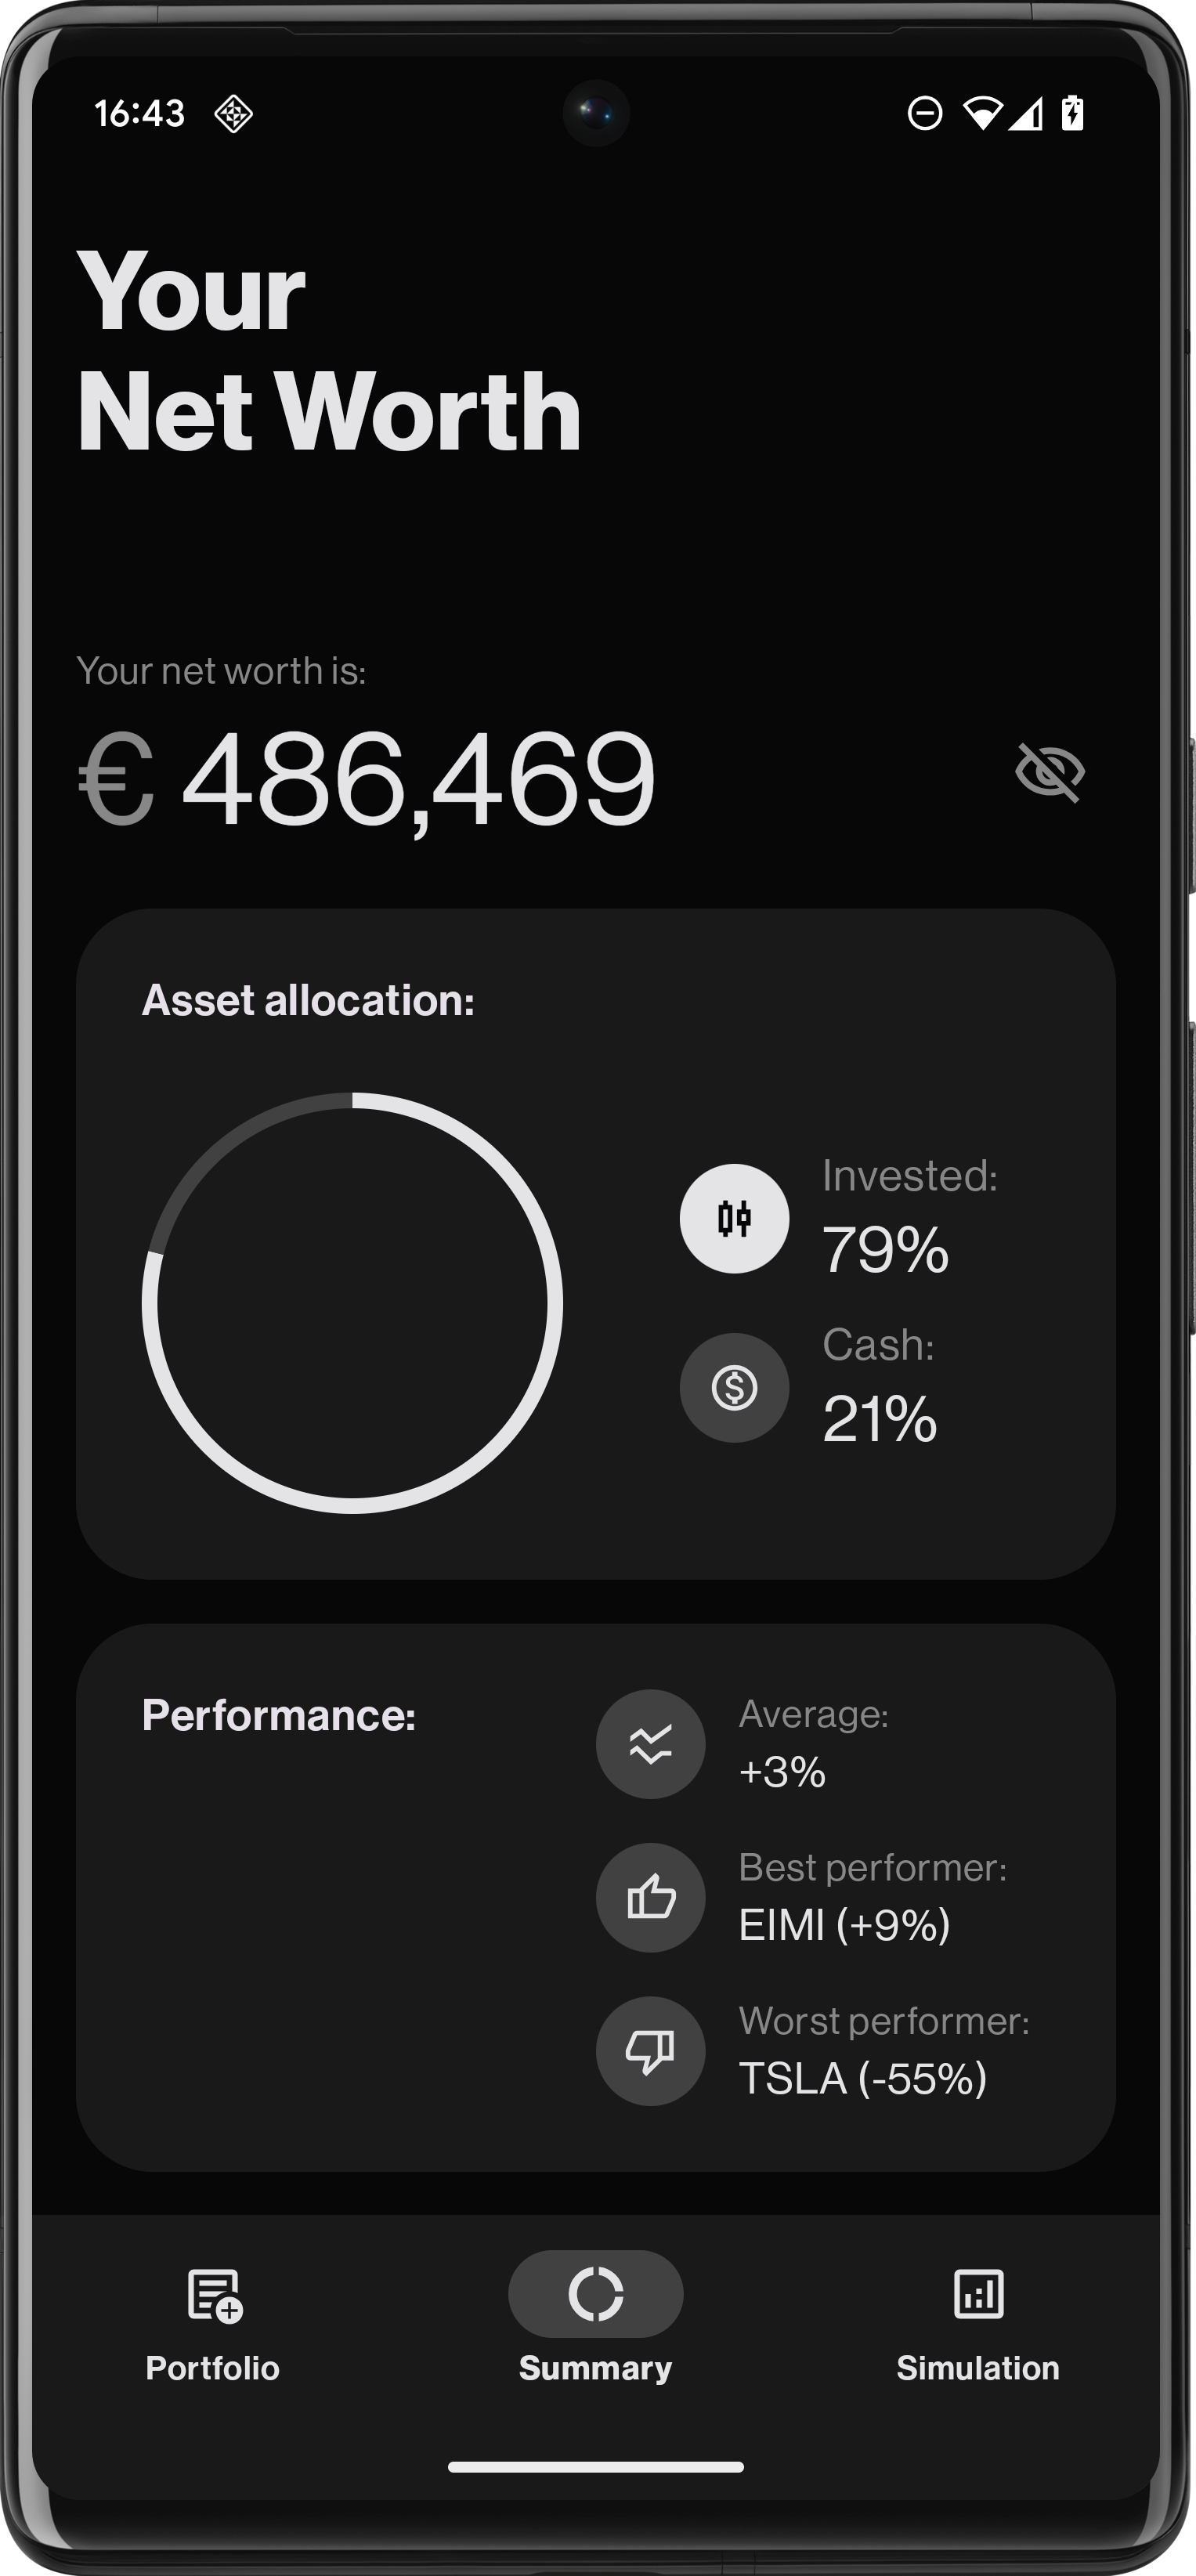
\includegraphics[width=\textwidth]{foto/summary_screen}
        \label{fig:summary_screen}
    \end{minipage}
\end{figure}

\begin{figure}[H]
    \centering
    \begin{minipage}{0.24\textwidth}
        \centering
        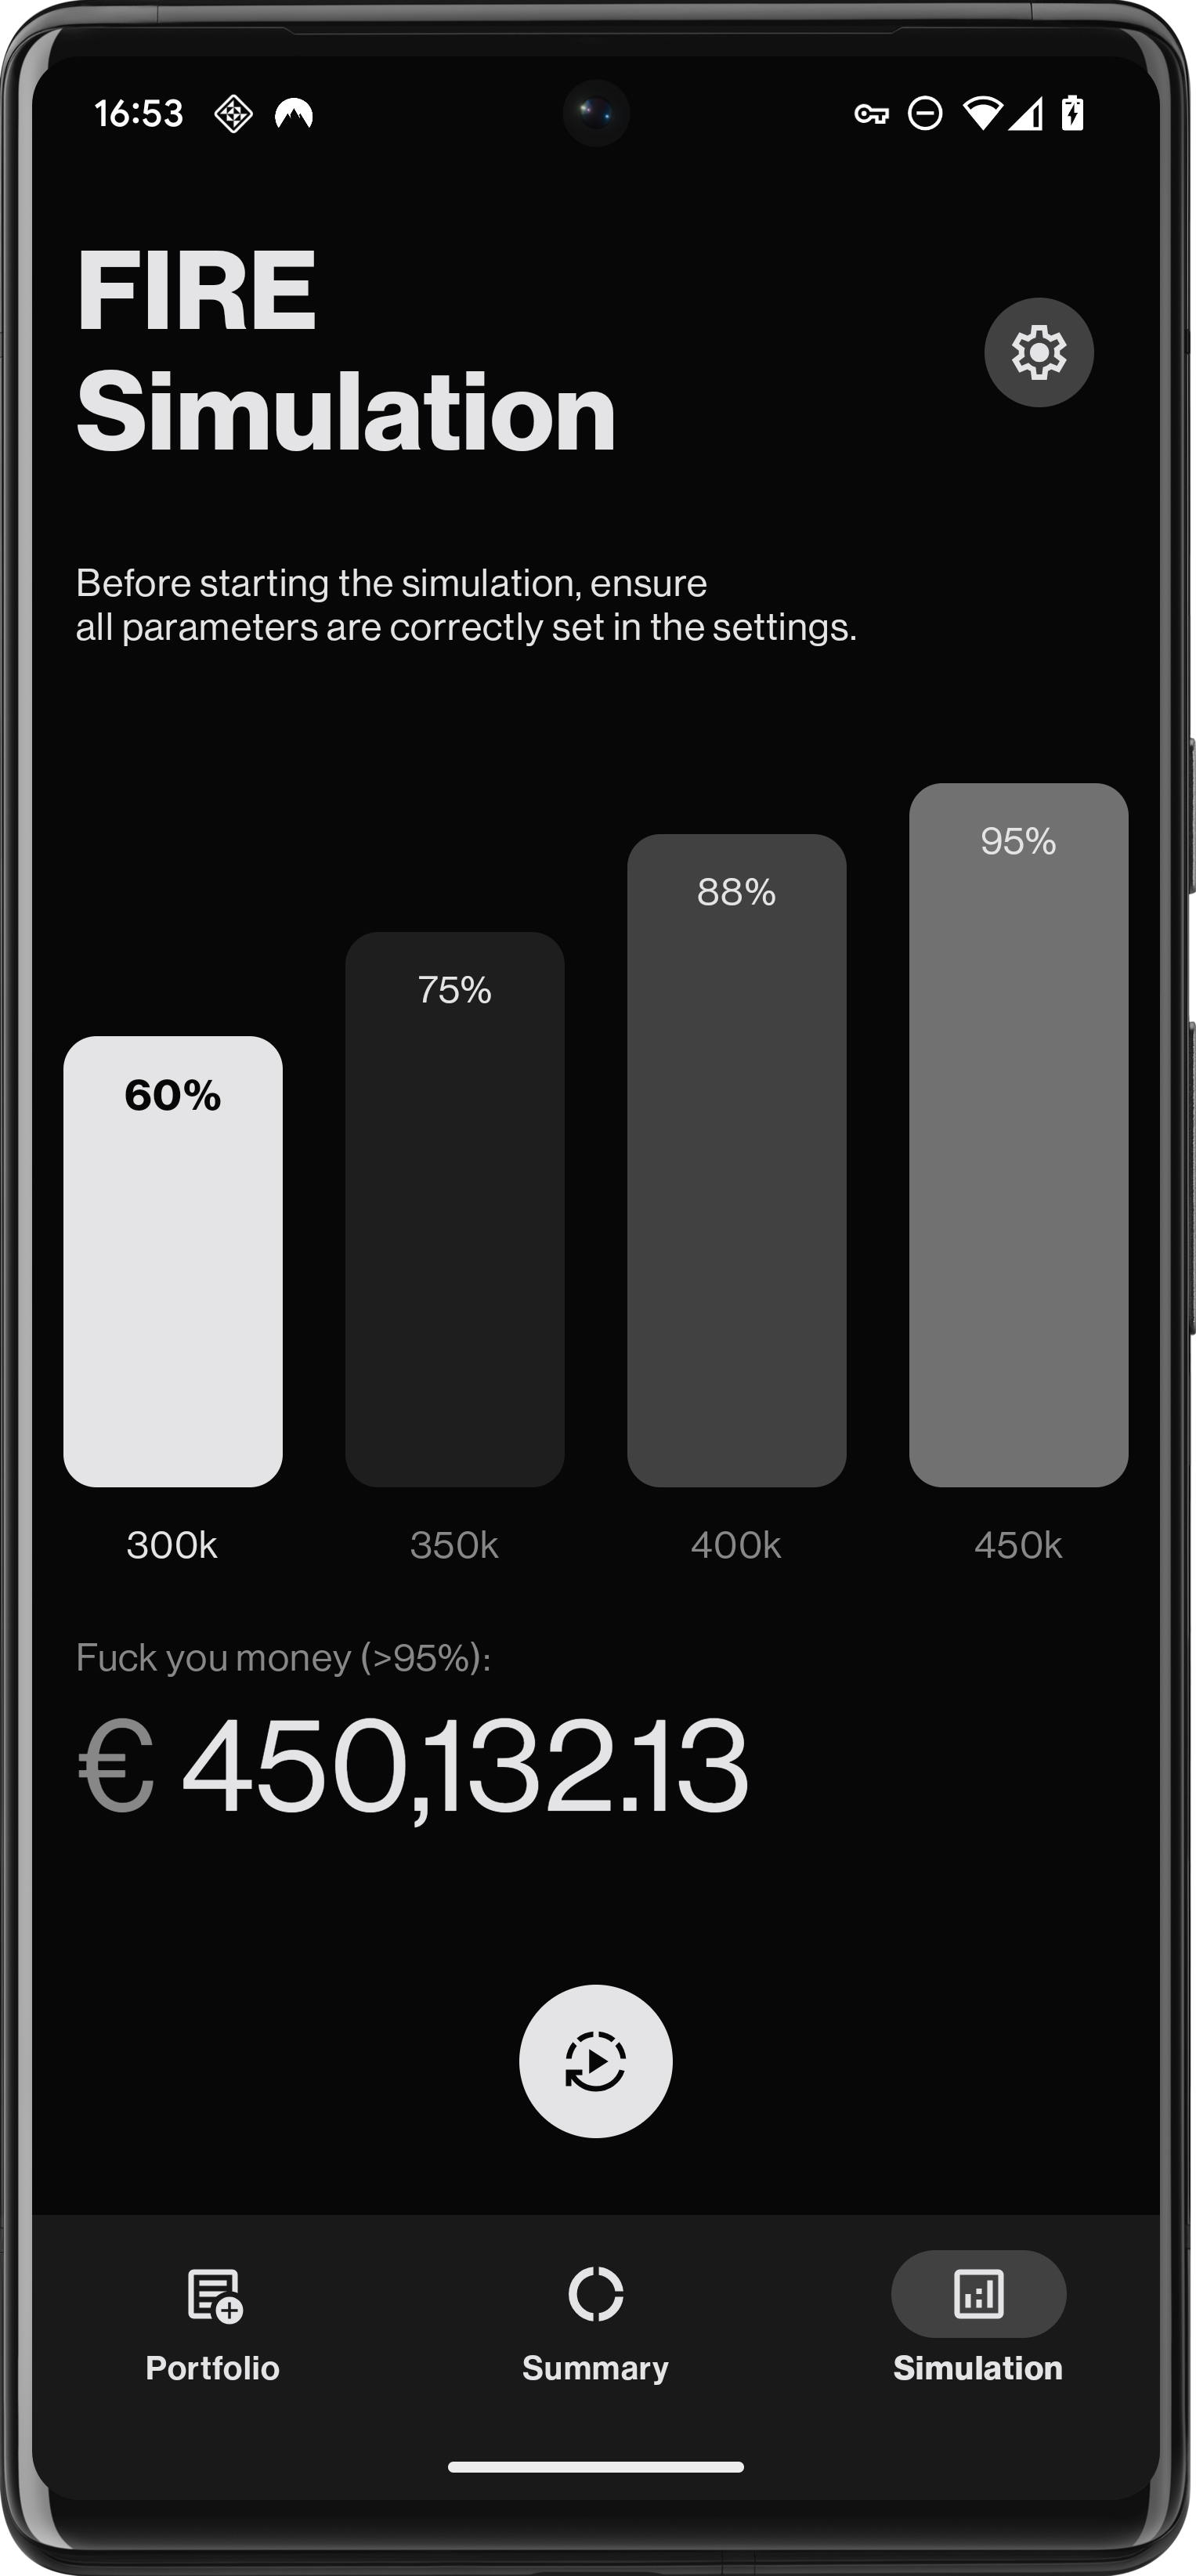
\includegraphics[width=\textwidth]{foto/simulation_screen}
        \label{fig:simulation_screen}
    \end{minipage}
    \hfill
    \begin{minipage}{0.24\textwidth}
        \centering
        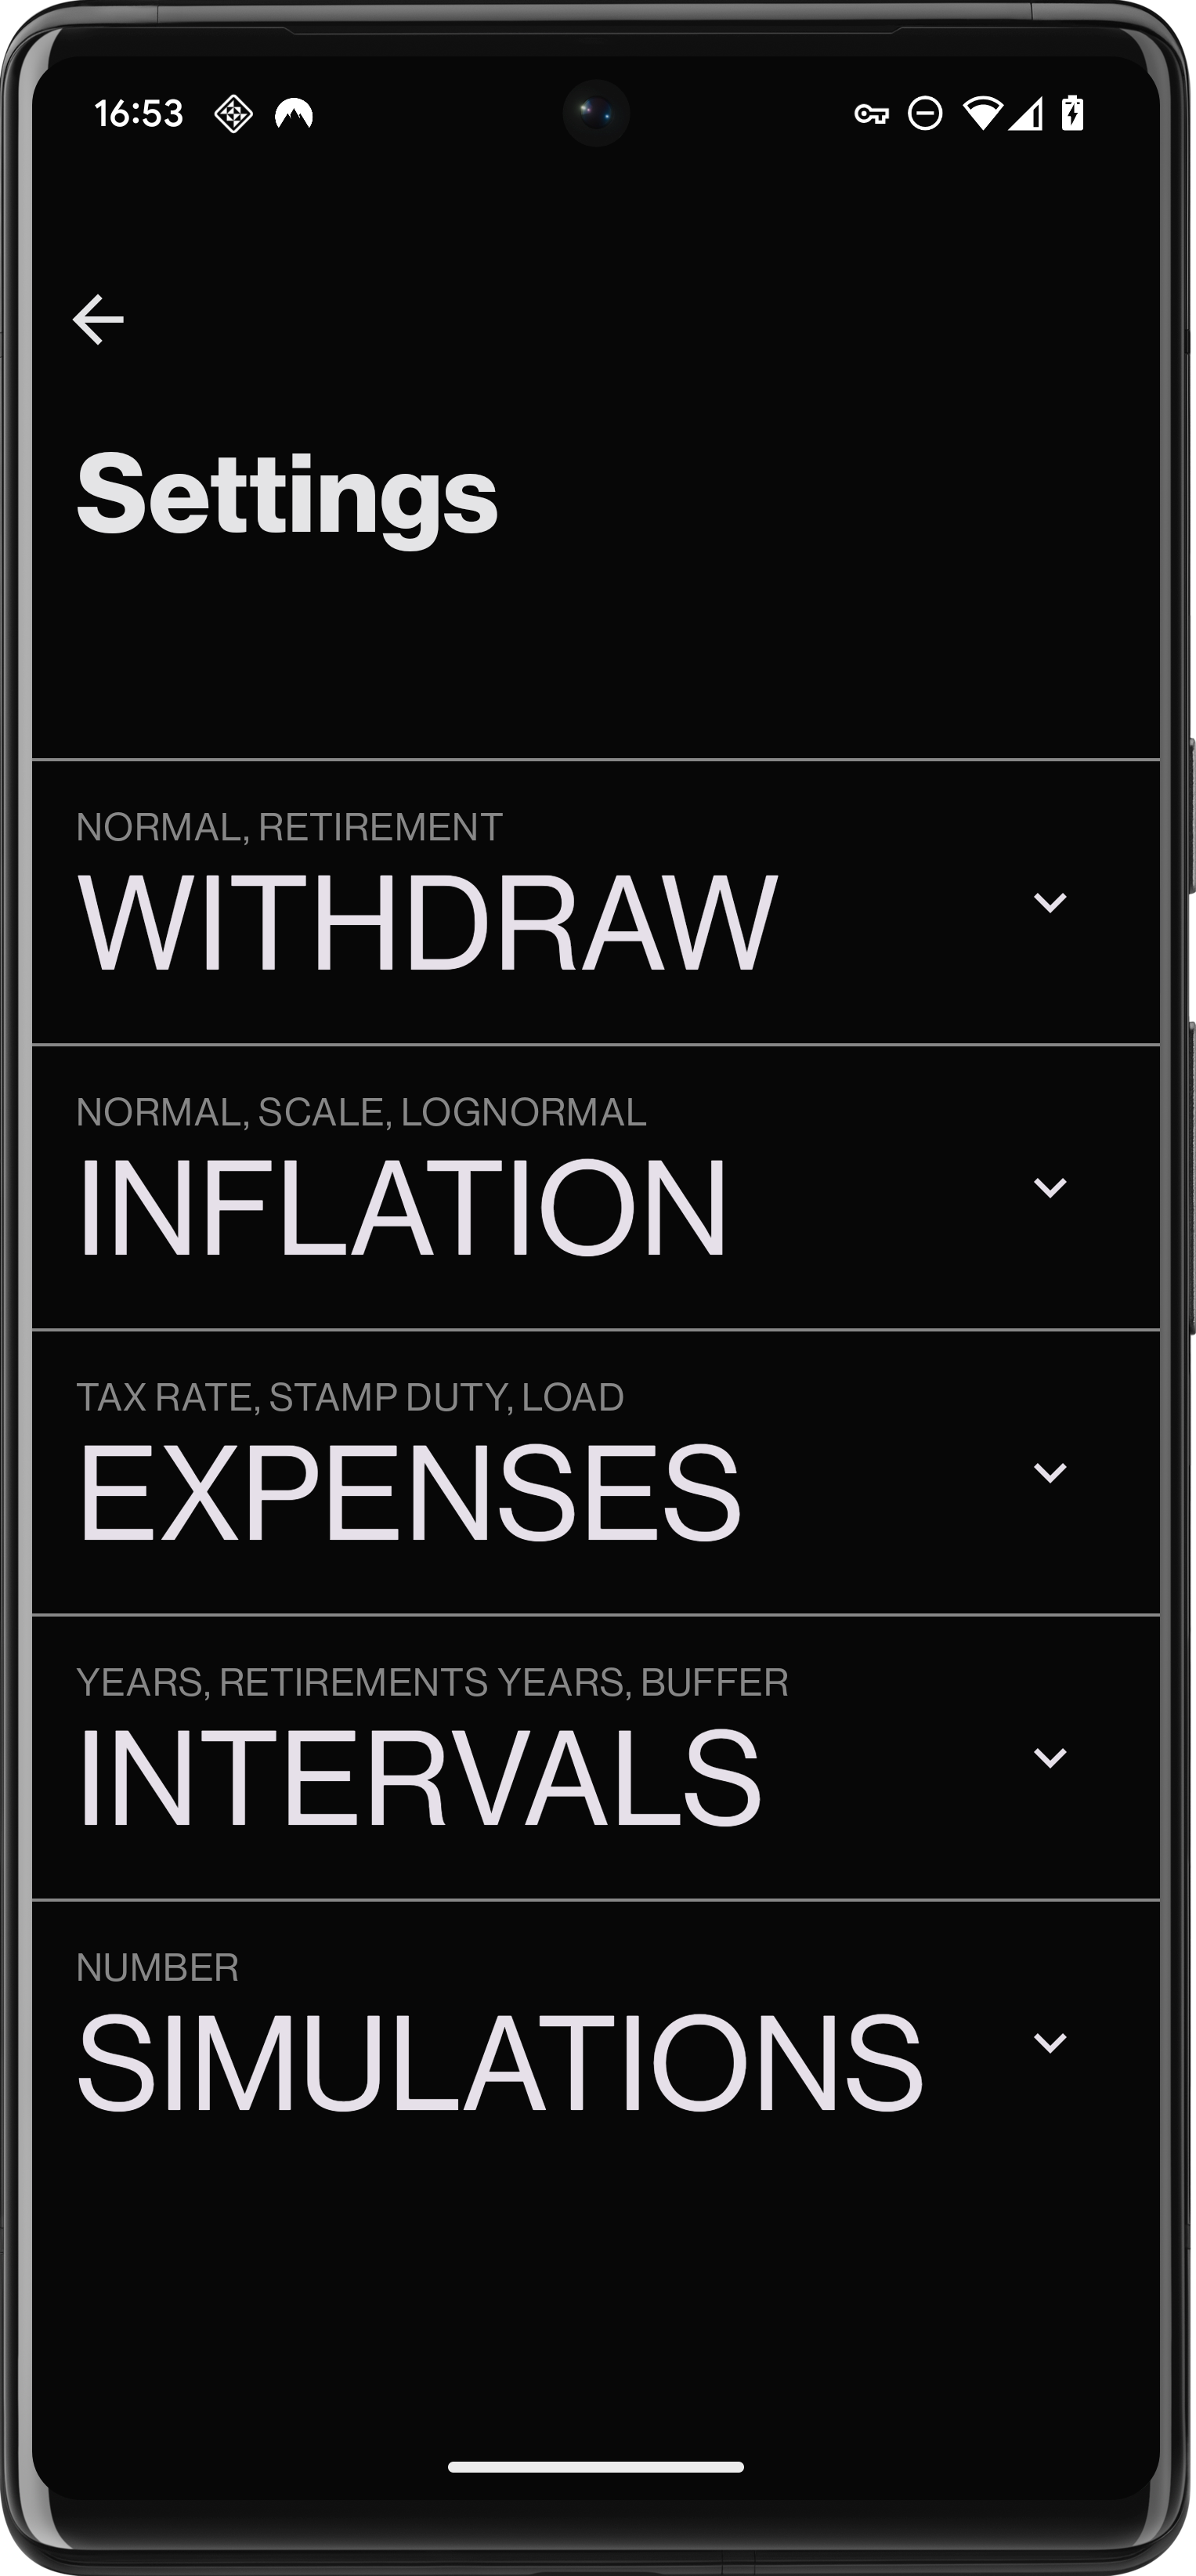
\includegraphics[width=\textwidth]{foto/settings_screen}
        \label{fig:settings_screen}
    \end{minipage}
    \hfill
    \begin{minipage}{0.24\textwidth}
        \centering
        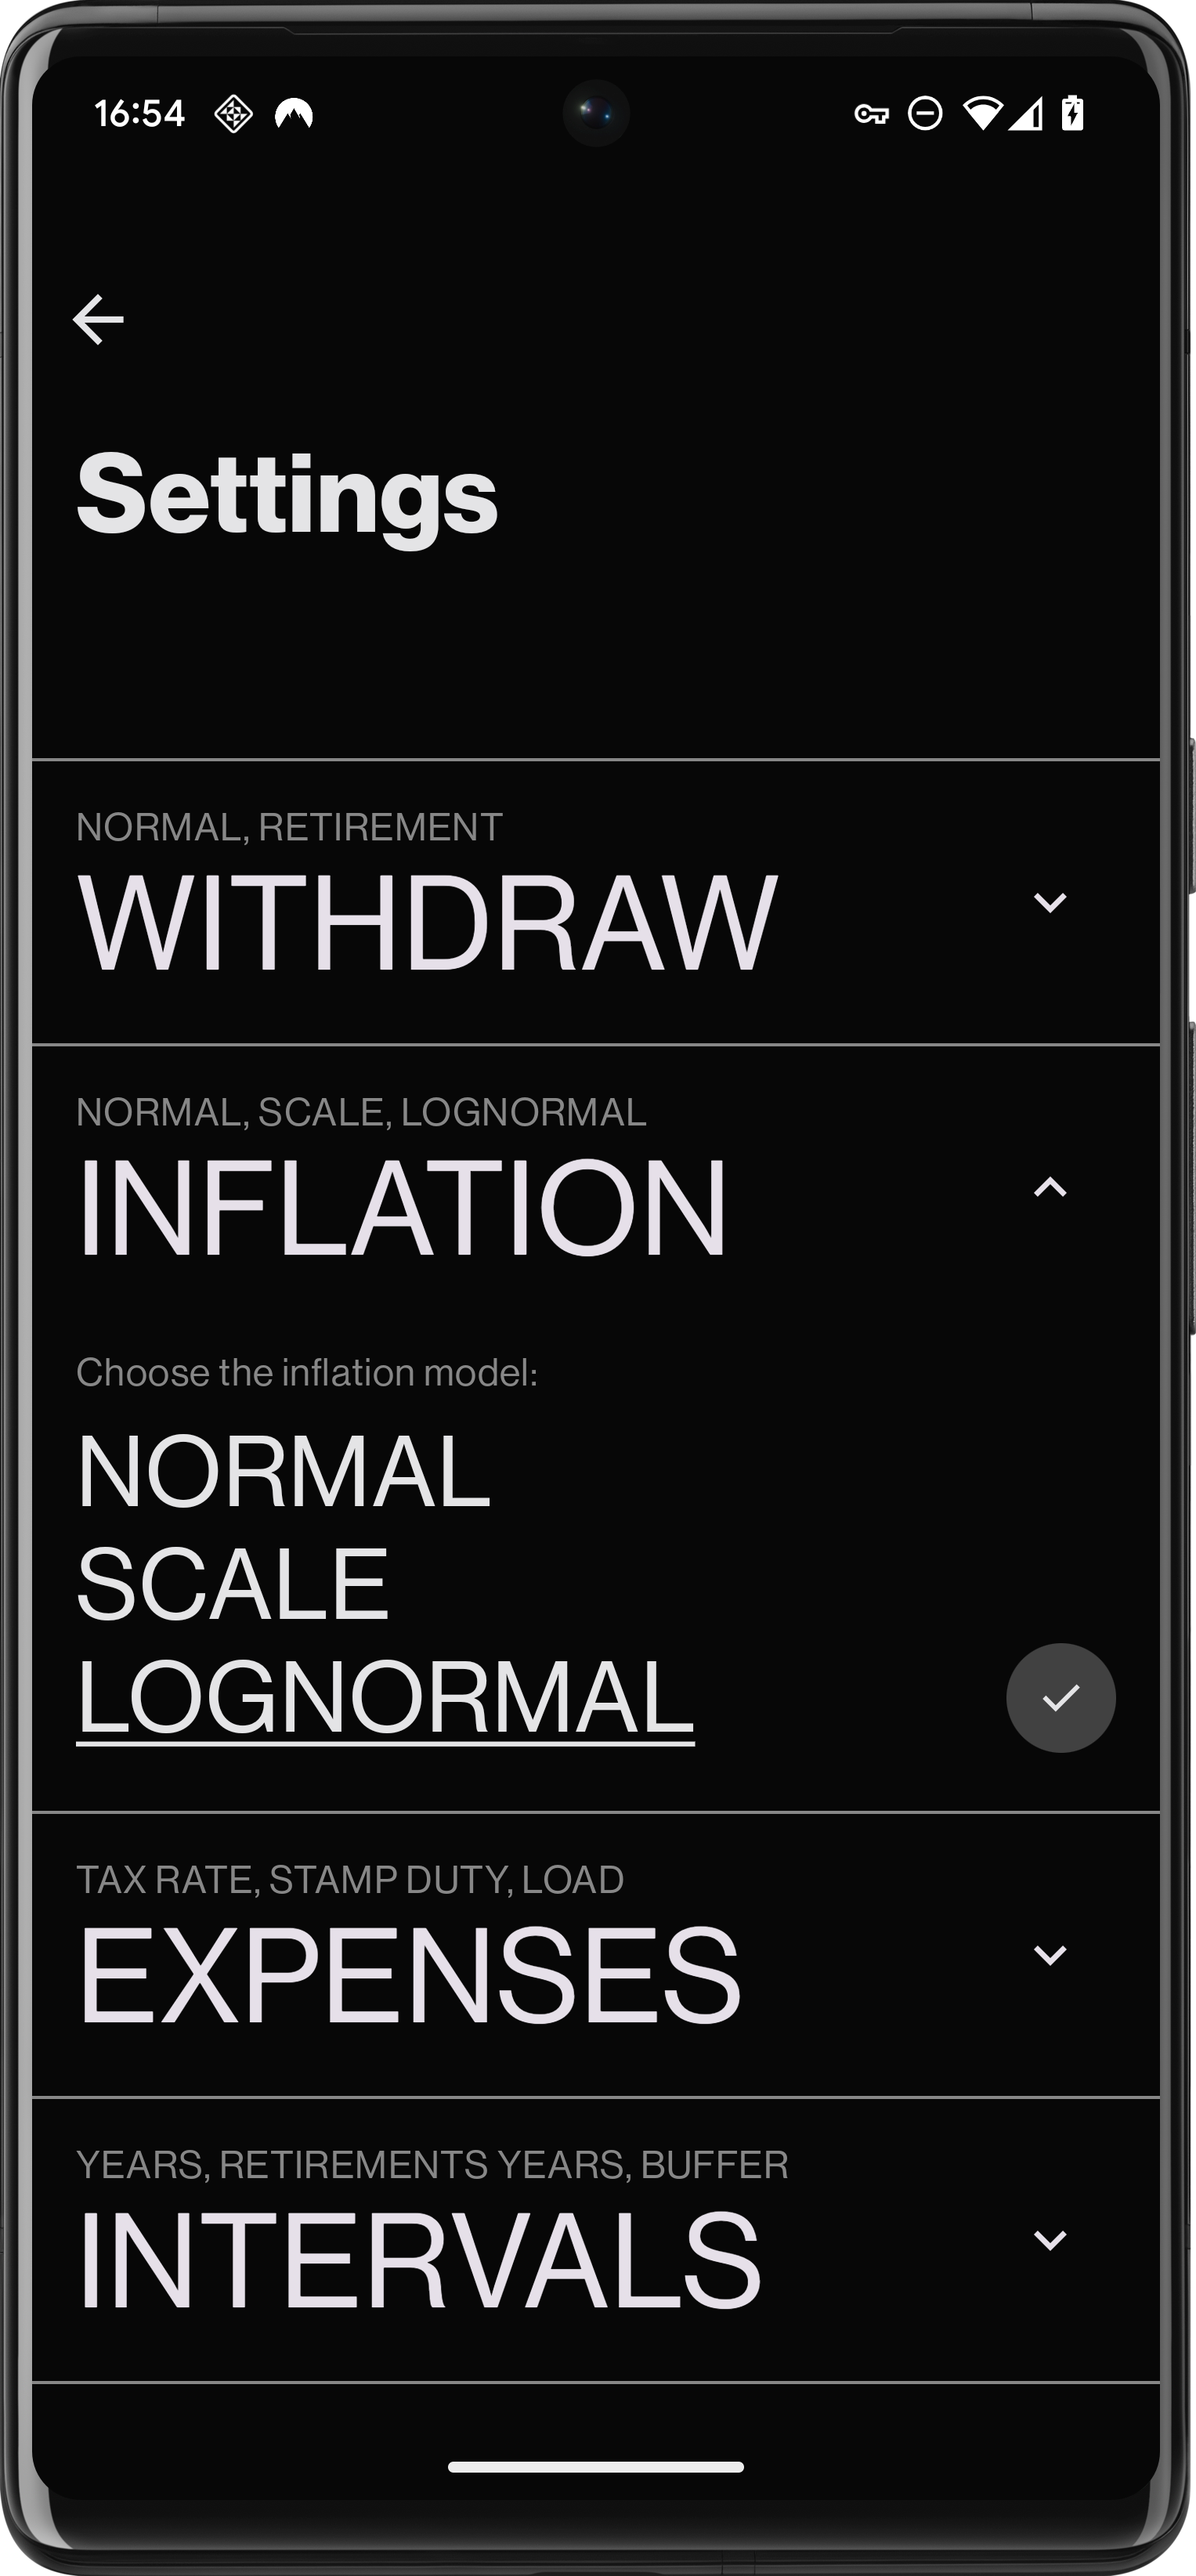
\includegraphics[width=\textwidth]{foto/inflation_card}
        \label{fig:inflation_card}
    \end{minipage}
    \hfill
    \begin{minipage}{0.24\textwidth}
        \centering
        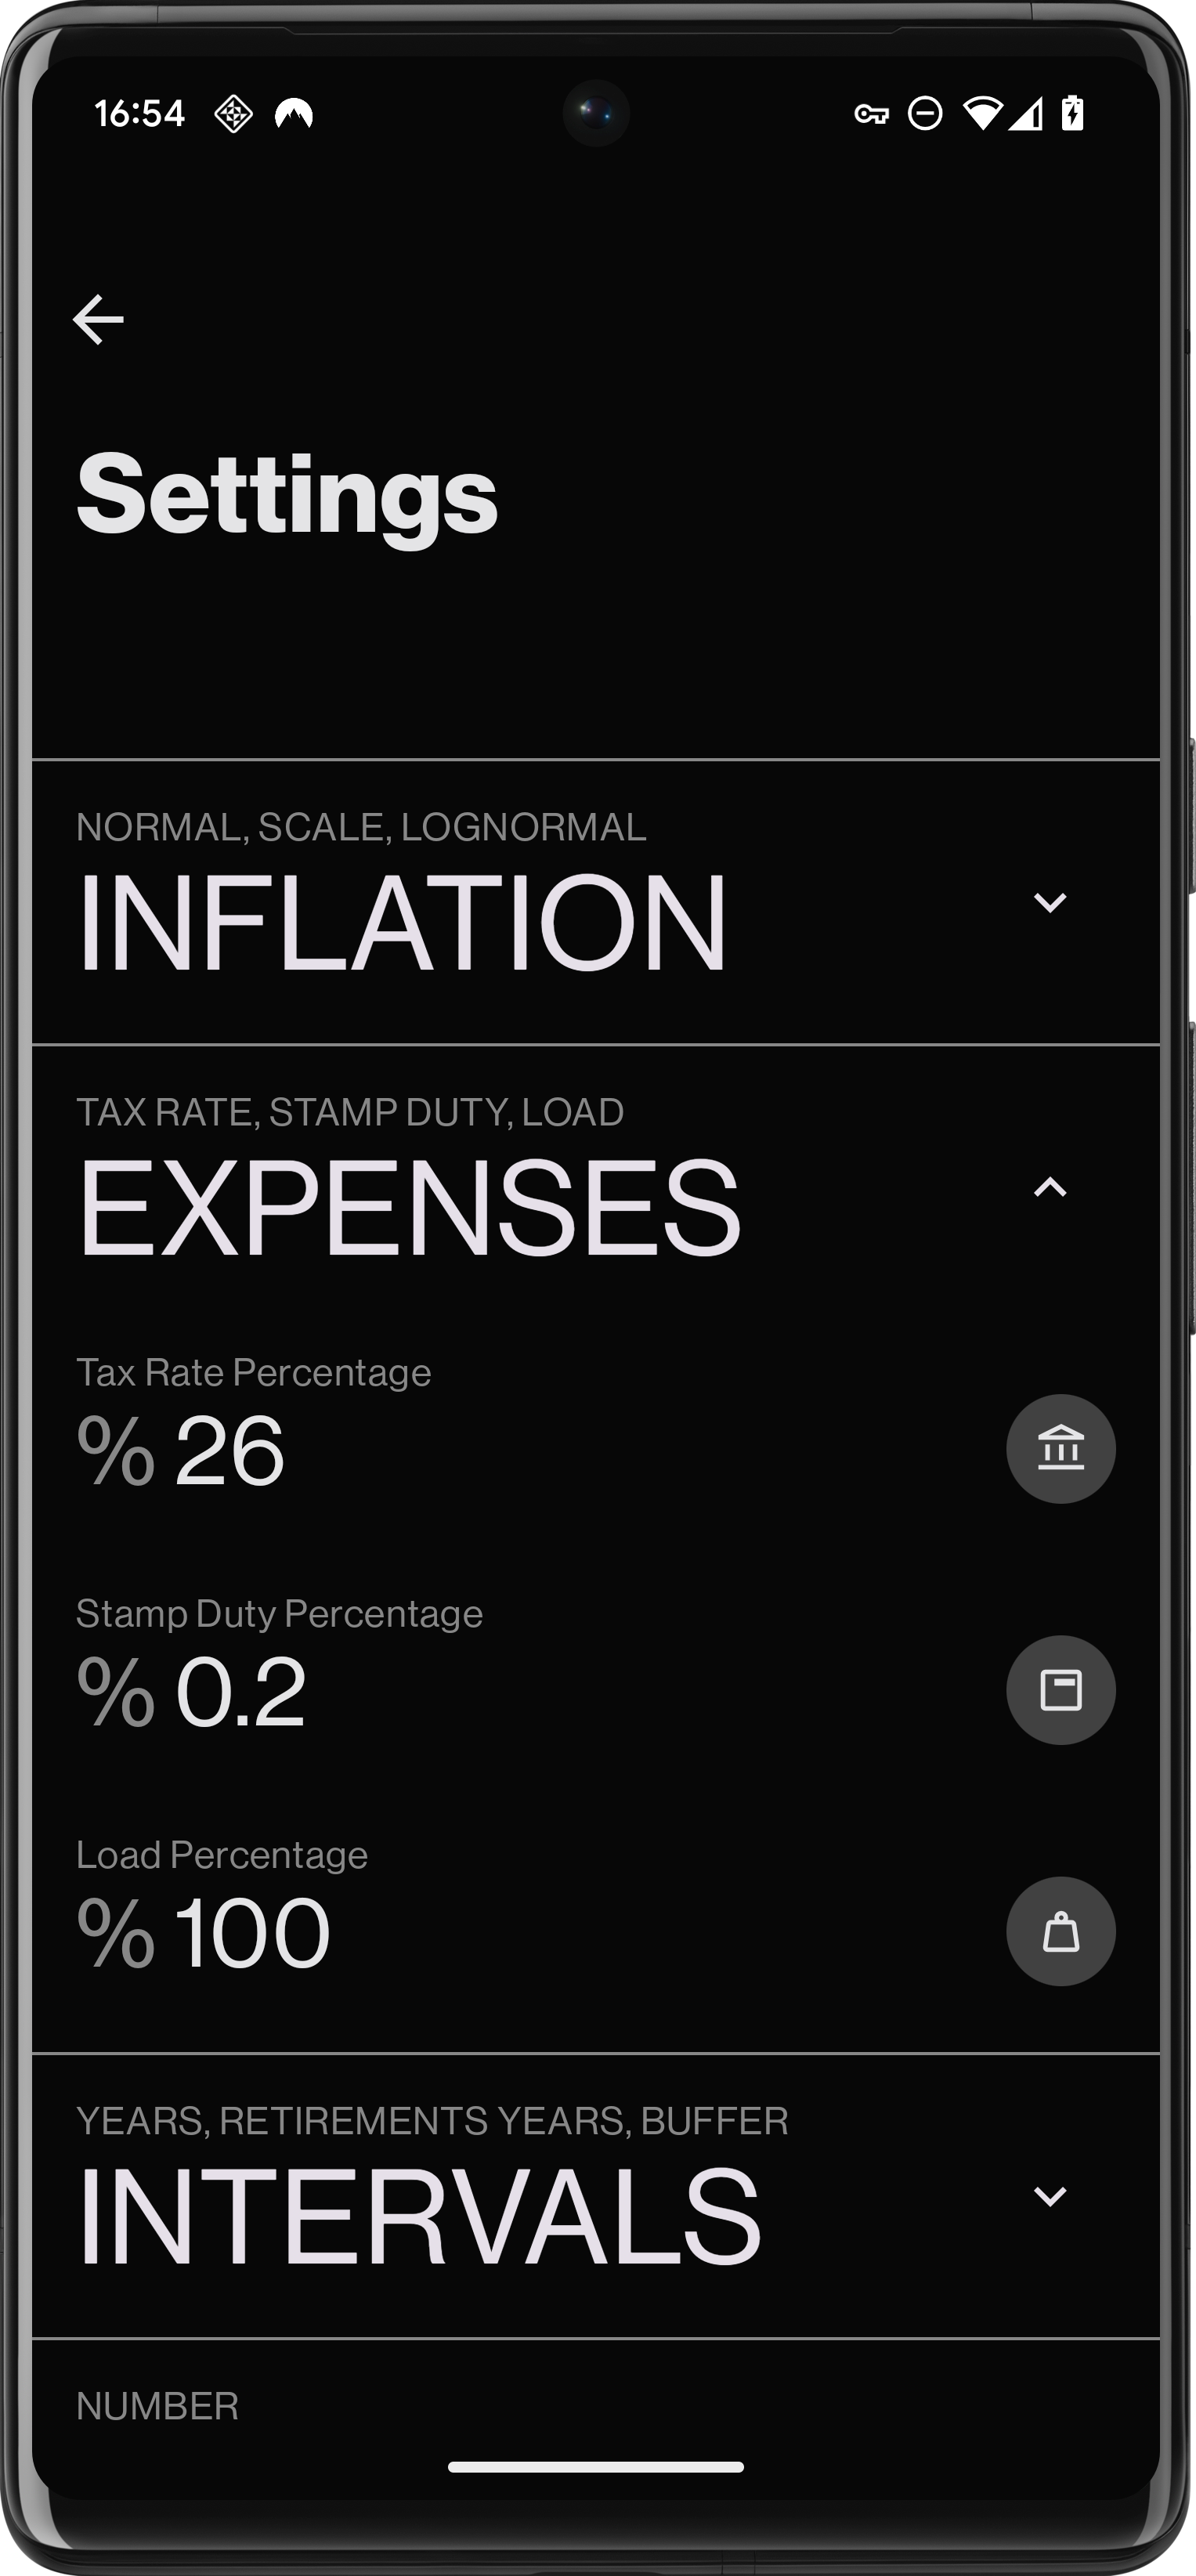
\includegraphics[width=\textwidth]{foto/input_card}
        \label{fig:input_card}
    \end{minipage}
\end{figure}

\section*{Conclusioni}
\addcontentsline{toc}{section}{Conclusioni}

Il progetto Ignition Finance ha rappresentato una sfida complessa e stimolante,
affrontata con l'obiettivo di creare un'applicazione mobile completa per la
pianificazione finanziaria e il raggiungimento dell'indipendenza finanziaria
(FIRE).  Attraverso un'architettura modulare e ben definita, l'applicazione
integra diverse componenti chiave, tra cui un sistema di persistenza locale
basato su Room, interazioni con API esterne per l'ottenimento di dati finanziari
in tempo reale, un'autenticazione sicura tramite Firebase Authentication e un
sistema di sincronizzazione dati locale-remoto robusto basato su Android
WorkManager.

\subsection*{Risultati Chiave e Punti di Forza}

Tra i principali risultati ottenuti, desideriamo evidenziare:

\begin{itemize}
    \item \textbf{Architettura Scalabile e Manutenibile:}  La suddivisione in
    moduli (\texttt{data}, \texttt{domain}, \texttt{presentation}, \texttt{di})
    ha permesso un approccio di sviluppo parallelo e una chiara separazione
    delle responsabilità, facilitando la manutenzione e l'estensione futura
    dell'applicazione.
    \item \textbf{Integrazione con Servizi Esterni:} L'integrazione con Firebase
    (Authentication e Firestore) e API finanziarie (Alpha Vantage, BCE) ha
    arricchito l'applicazione con funzionalità avanzate e dati aggiornati.
    \item \textbf{Simulazione FIRE Avanzata:} L'implementazione di un algoritmo
    di simulazione FIRE completo, in grado di tenere conto di diversi scenari
    economici e strategie di prelievo, fornisce agli utenti uno strumento
    prezioso per la pianificazione finanziaria a lungo termine.
    \item \textbf{Sincronizzazione Dati Affidabile:} Il sistema di
    sincronizzazione dati locale-remoto, basato su Android WorkManager e una
    coda di sincronizzazione gestita localmente, garantisce la consistenza dei
    dati anche in condizioni di connettività intermittente.
    \item \textbf{Interfaccia Utente Moderna e Reattiva:} L'utilizzo di Jetpack
    Compose ha permesso la creazione di un'interfaccia utente moderna, intuitiva
    e reattiva, offrendo un'esperienza utente fluida e coinvolgente.
\end{itemize}

\subsection*{Sfide Incontrate e Lezioni Apprese}

Lo sviluppo di Ignition Finance non è stato privo di sfide.
Tra le principali,
ricordiamo:

\begin{itemize}
    \item \textbf{Gestione della Complessità dei Dati Finanziari:} La gestione
    di dati finanziari complessi e la loro integrazione con l'algoritmo di
    simulazione FIRE ha richiesto un'attenta progettazione e validazione.
    \item \textbf{Sincronizzazione Dati in Ambienti con Connettività Variabile:}
    Garantire la consistenza dei dati in ambienti con connettività intermittente
    ha rappresentato una sfida significativa, superata attraverso
    l'implementazione di un sistema di sincronizzazione dati robusto e
    resiliente.
    \item \textbf{Ottimizzazione delle Performance:} L'esecuzione di simulazioni
    FIRE complesse può richiedere risorse computazionali significative.
    L'ottimizzazione delle performance è stata una priorità costante durante lo
    sviluppo.
    \item \textbf{Gestione dei Conflitti di Sincronizzazione:} Implementare una
    strategia efficace per la gestione dei conflitti durante la sincronizzazione
    dei dati tra locale e remoto, in particolare per le operazioni di
    aggiornamento, ha richiesto un'analisi approfondita e l'implementazione di
    meccanismi di controllo basati su timestamp.
\end{itemize}

Queste sfide ci hanno permesso di acquisire preziose lezioni, rafforzando la
nostra comprensione delle problematiche legate allo sviluppo di applicazioni
finanziarie mobile e consolidando le nostre competenze nell'ambito delle
architetture software complesse.

\subsection*{Sviluppi Futuri e Prospettive}

Il progetto Ignition Finance rappresenta una solida base per futuri sviluppi e
miglioramenti.
Tra le possibili direzioni future, suggeriamo:

\begin{itemize}
    \item \textbf{Ampliamento delle Funzionalità di Simulazione FIRE:} Integrare
    ulteriori parametri e scenari nella simulazione FIRE, come ad esempio la
    possibilità di considerare diverse fonti di reddito, spese impreviste e
    l'impatto di eventi macroeconomici.
    \item \textbf{Integrazione con Ulteriori API Finanziarie:}  Aggiungere il
    supporto per ulteriori API finanziarie per l'ottenimento di dati più
    specifici e dettagliati, come ad esempio informazioni su fondi comuni di
    investimento, ETF e obbligazioni.
    \item \textbf{Personalizzazione Avanzata dell'Asset Allocation:} Offrire
    agli utenti la possibilità di personalizzare l'asset allocation del proprio
    portafoglio in modo più granulare, consentendo la creazione di strategie di
    investimento più sofisticate.
    \item \textbf{Supporto per la Pianificazione Fiscale:} Integrare
    funzionalità di pianificazione fiscale per aiutare gli utenti a ottimizzare
    la propria strategia finanziaria dal punto di vista fiscale.
    \item \textbf{Miglioramento dell'Interfaccia Utente:} Continuare a
    migliorare l'interfaccia utente, rendendola ancora più intuitiva e
    accessibile, e implementare nuove funzionalità basate sul feedback degli
    utenti.
    \item \textbf{Implementazione di un sistema di notifica più proattivo:}
    Integrare un sistema di notifica che avvisi l'utente in caso di eventi
    significativi che potrebbero influenzare il suo percorso verso
    l'indipendenza finanziaria (es: forti ribassi di mercato, superamento di
    determinate soglie di spesa, etc.).
\end{itemize}

In conclusione, Ignition Finance rappresenta un progetto di successo che ha
dimostrato la nostra capacità di affrontare sfide complesse e di creare
un'applicazione mobile innovativa e di valore per gli utenti.
Siamo convinti
che, con ulteriori sviluppi e miglioramenti, Ignition Finance possa diventare
uno strumento indispensabile per chiunque desideri pianificare il proprio futuro
finanziario e raggiungere l'indipendenza finanziaria.\\
E ricordate Ignition Finance non è solo un'app, è uno stile di vita!

\end{document}